% !TeX program = pdflatex
% !TeX encoding = UTF-8
\documentclass[12pt,a4paper,oneside]{article}
\usepackage[utf8]{inputenc}
\usepackage[T1]{fontenc}
\usepackage[provide=*,main=spanish]{babel}
\addto\captionsspanish{\renewcommand{\tablename}{Tabla}\renewcommand{\refname}{Referencias}\renewcommand{\listtablename}{Índice de tablas}}
\usepackage{lmodern,microtype,amsmath,amssymb,booktabs,longtable,array,graphicx,xcolor}
\usepackage[left=25mm,right=25mm,top=24mm,bottom=24mm,headheight=14pt]{geometry}
\usepackage{lscape}
\usepackage{setspace,enumitem,caption,float,fancyhdr,titlesec,tikz,needspace}
\usetikzlibrary{arrows.meta,positioning}
\usepackage[hidelinks,pdfauthor={Sebastián Felipe Porras Rincón},pdftitle={Mejora del sistema de producción en la empresa RPM Colombia S.A.S. mediante modelos de gerencia de operaciones}]{hyperref}
\setstretch{1.12}
\clubpenalty=10000
\widowpenalty=10000
\setlength{\parindent}{0pt}\setlength{\parskip}{5pt}
\setlist{nosep,leftmargin=*}
\captionsetup{font=small,labelfont=bf,skip=6pt}
\definecolor{azul}{HTML}{233B54}
\titleformat{\section}{\large\bfseries}{\thesection.}{.6em}{}
\titleformat{\subsection}{\normalsize\bfseries}{\thesubsection.}{.6em}{}
\titlespacing*{\section}{0pt}{14pt}{7pt}
\titlespacing*{\subsection}{0pt}{10pt}{4pt}
\pagestyle{fancy}\fancyhf{}\fancyhead[L]{\small RPM Colombia S.A.S.}\fancyhead[R]{\small Planificación de la producción}\fancyfoot[C]{\thepage}
\renewcommand{\headrulewidth}{.3pt}
\newcommand{\fuente}[1]{\par\vspace{3pt}{\footnotesize\textit{Fuente: #1.}\par}}
\newcommand{\num}[1]{\ensuremath{#1}}
\makeatletter\renewcommand{\@pnumwidth}{3em}\renewcommand{\@tocrmarg}{4em}\makeatother
\begin{document}
\hypersetup{pageanchor=false}
\begin{titlepage}
\thispagestyle{empty}
\begin{center}

\includegraphics[width=75mm]{figuras/logo_color.pdf}\par
\vspace{9mm}
{\large Facultad de Ingeniería}\par
Maestría en Ingeniería Industrial\par
\vspace{21mm}
{\LARGE\bfseries Mejora del sistema de producción en la empresa RPM Colombia S.A.S. mediante modelos de gerencia de operaciones\par}
\vspace{19mm}
{\large\bfseries Sebastián Felipe Porras Rincón}\par
\vspace{5mm}
Trabajo de grado para optar al título de\par
Magíster en Ingeniería Industrial\par
\vspace{17mm}
Director\par
{\large David Álvarez Martínez}\par
\vfill
Bogotá, Colombia\par
2026
\end{center}
\end{titlepage}
\pagenumbering{roman}
\hypersetup{pageanchor=true}
\begingroup\setstretch{1.0}\tableofcontents\endgroup
\clearpage
\listoffigures
\clearpage
\listoftables
\clearpage
\pagenumbering{arabic}
\begin{center}
{\Large\bfseries Mejora del sistema de producción en la empresa RPM Colombia S.A.S. mediante modelos de gerencia de operaciones\par}
\vspace{3mm}
Sebastián Felipe Porras Rincón\par
{\small Universidad de los Andes · Maestría en Ingeniería Industrial}
\end{center}
\section*{Resumen}
La compañía RPM Colombia S.A.S. enfrenta el problema de asignar referencias a máquinas cuyas capacidades y tiempos de alistamiento difieren. En este trabajo proponemos un modelo de programación lineal entera mixta que busca minimizar la carga agregada de producción y comparamos los planes que éste produce con los de una heurística usada por la compañía. Enfocamos nuestra evaluación en el análisis de 100 instancias sintéticas donde se varía la intensidad de la demanda, el tamaño del catálogo de productos, el horizonte, la capacidad de las máquinas y la matriz de tiempos de alistamiento. El generador de instancias remuestrea los factores relativos de ventas semestrales dentro de estratos de volumen, de modo que se logra una representación de la heterogeneidad entre productos, pero no se asigna una variabilidad diaria que no puede estimarse con los datos disponibles. Para cada instancia ejecutamos una vez el algoritmo heurístico de referencia y los solvers CBC, HiGHS y Gurobi (sin proporcionarles una solución inicial). Verificamos los resultados obtenidos para asegurar que todas las restricciones sean respetadas, y determinamos, para cada instancia, si la solución es completa, si se obtuvo un certificado numérico de optimalidad o si la instancia es inviable. Gurobi logró encontrar solución en los 76 problemas donde existía una, y pudo garantizar la optimalidad en 41 de estos. Todos los planes completos obtenidos por Gurobi tienen GAP menor al 0.18\,\%. En comparación con la heurística, en las instancias donde ésta es capaz de obtener un plan que cubre toda la demanda, logramos una reducción promedio de la carga agregada cercana al 22\,\% (incluyendo los incumbentes para los que no se logró certificar la optimalidad). Estos resultados sugieren que es más efectivo realizar una asignación conjunta de las referencias y dan una idea de las limitaciones de una heurística local en la toma de decisiones cuando existe competencia por capacidad. También se presentan casos nominales y Monte Carlo histórico para complementar la evidencia presentada y con alcance distinto. La mejora que logramos es en el modelo de producción, pero no se reporta una medición en ahorro económico obtenido en la planta.

\textbf{Palabras clave:} programación entera mixta; asignación de producción; capacidad; alistamiento; certificación de optimalidad.
\par\medskip
\Needspace{6\baselineskip}
\noindent\textbf{Abstract}\par\smallskip
\noindent
RPM Colombia S.A.S. assigns products to machines with different capacities, processing times, and setup requirements. This work formulates a mixed integer linear programming model that minimizes the aggregate production load and compares its production plans with a reference heuristic. The main experiment studies 100 synthetic instances with different demand intensity, product catalogue size, planning horizon, machine capacity, and processing time matrix. The synthetic demand generator resamples the relative sales factors per semester within demand volume strata. The generated instances capture variability among products, but not daily demand variability, which could not be identified in the available data. Each instance is run once with the heuristic and once with CBC, HiGHS, and Gurobi, and no starting solution is inherited by any run. An audit of the exported production plans classifies them as feasible and complete, and distinguishes numerical optimality certificates from infeasible plans. Gurobi finishes with a known feasible solution for all 76 problems with a feasible solution, and verifies optimality for 41 of them. All complete production plans have a final gap lower than 0.18\,\%. Gurobi's production plans, which cover all the demand, have an average load reduction with respect to the heuristic's of around 22\,\%, even counting incumbent solutions without an optimality certificate. These results support a joint allocation of products, and point out limitations of the local rule when products compete for capacity. Additional supporting evidence is presented on nominal examples and using Monte Carlo methods on historical data. The presented improvements relate to the workload modeled; financial savings at the shop floor are not measured.

\section{Problema de decisión y propósito del estudio}
RPM Colombia, es una empresa encargada de la producción de artículos plásticos por encargo. Cuenta con diez máquinas de producción que operan en turnos. Los supervisores de las máquinas, utilizan su experiencia y conocimiento del negocio para asignar las referencias según el volumen a producir, las prioridades de la empresa y la disponibilidad de las maquinas. El conocimiento es un elemento fundamental en la operación y por ello este modelo busca complementar el proceso con un criterio cuantificable que pueda comparar opciones y brindar trazabilidad del proceso de asignación de referencias.

La decisión radica en establecer qué día y cuántas unidades de cada referencia ha de producir una máquina en un horizonte multiperiodo. Una máquina con menor tiempo unitario puede requerir un gran alistamiento o absorber capacidad que otra referencia requiera, por lo que no basta con optar por el menor tiempo unitario de forma aislada. El modelo tiene en cuenta de manera conjunta la demanda, el procesamiento, la preparación y la disponibilidad nominal.

El fin último es plantear y someter a evaluación un modelo de asignación que reduzca al mínimo la carga nominal para dar respuesta a la demanda. A tal efecto, el trabajo persigue cuatro objetivos: caracterizar el rendimiento de cada máquina y referencia; poner de relieve unos indicadores para la interpretación de la asignación; definir la función objetivo junto con sus variables y restricciones; y, tras valorar los resultados, ofrecer criterios de planificación a RPM Colombia. Las expresiones son lineales, pero las cantidades enteras y las activaciones binarias hacen que la formulación sea un MILP.

La cuestión de investigación que se plantea es \textit{qué tipo de asignación de cantidades permite satisfacer la demanda y respetar la capacidad de que se dispone, todo ello reduciendo la carga de preparación y procesamiento, y con qué pruebas se puede defender su optimalidad}. Para abordar esta cuestión, se consideran tres niveles: la calidad de los datos de entrada, la validez del modelo dentro de su ámbito y el hecho de que las soluciones han sido comprobadas por la computadora. El certificado de optimalidad lo que garantiza es que los resultados son óptimos para los parámetros y restricciones que figuran en el modelo, no que los tiempos de operación son correctos o que las combinaciones referencia-máquina son técnicamente compatibles.

El núcleo del análisis de este estudio reside en la comparación realizada utilizando cien instancias sintéticas basadas en la dispersión transversal de las ventas por referencia. En la sección~\ref{sec:instancias} se detalla el diseño de estas instancias y se presenta la comparación de la heurística con los tres motores sin un inicio heredado. Los dos casos nominales sirven para mostrar la formulación y sus certificados, y Monte Carlo histórico mantiene su alcance complementario. De esta forma se consigue no confundir las repeticiones de un mismo problema con la diversidad de demanda.

\subsection{Alcance operativo}
La capacidad del sistema se ha supuesto en 1.440 minutos diarios/máquina, aunque no se presenta en el expediente un calendario neto considerando las deducciones por mantenimiento, averías, paradas o insuficiencia de personal; por tanto el resultado se basa en esta capacidad disponible nominal. El responsable de planta debe verificar la capacidad neta disponible, los recursos de preparación y las compatibilidades antes de ejecutar una orden. Se trata de una decisión por cantidades y no de una secuenciación detallada. El modelo no considera las precedencias ni el momento exacto de inicio de ejecución. Tampoco considera tiempos de cambio de acuerdo a la secuencia, ni inventario al final de periodo, ni liberaciones de órdenes o entregas en un punto exacto. El modelo permite asignar una referencia a varias máquinas y días. El modelo considera un alistamiento para cada combinación activa de referencia, máquina y día. En este caso, el modelo considera alistamiento cada vez que la referencia es activa en una máquina cada día. No se considera una medida de alistamiento al comenzar el día. Si el alistamiento se mantiene en la planta, de un día a otro, debe modelarse y recalcularse.
La calidad y el desperdicio son indicadores gerenciales y el modelo no los optimiza por falta de información comparativa para máquinas y productos. El modelo asume que la demanda debe ser cumplida al 100\,\%. No es una prueba de que se mejora un indicador histórico de servicio. El cumplimiento de la demanda tampoco es una prueba de que hay mejoras en términos de defectos, costos o tiempos de entrega reales.

\section{Fundamentos y enfoque metodológico}
% !TeX root = ../Trabajo_RPM.tex
En este trabajo se vinculan los datos de RPM a decisiones de asignación comprobables. En la Fig.~\ref{fig:ruta_metodologica_rpm}, se ilustra la diferencia entre el estudio de los cien problemas y los dos casos nominal y Monte Carlo histórico. El estudio en común entre ambos casos es que se realizaron a partir de 25 vectores de demanda. Con cada vector de demanda se obtuvo 4 variantes para capacidad y matriz. Cada uno de los caminos presenta sus protocolos y resultados particulares.

\begin{landscape}
\thispagestyle{plain}
\begin{figure}[H]
\centering
{\Large\bfseries\color{azul} Datos, instancias y validación\par}
\vspace{3mm}
{\small Comparación y análisis complementarios sobre las matrices de RPM\par}
\vspace{8mm}
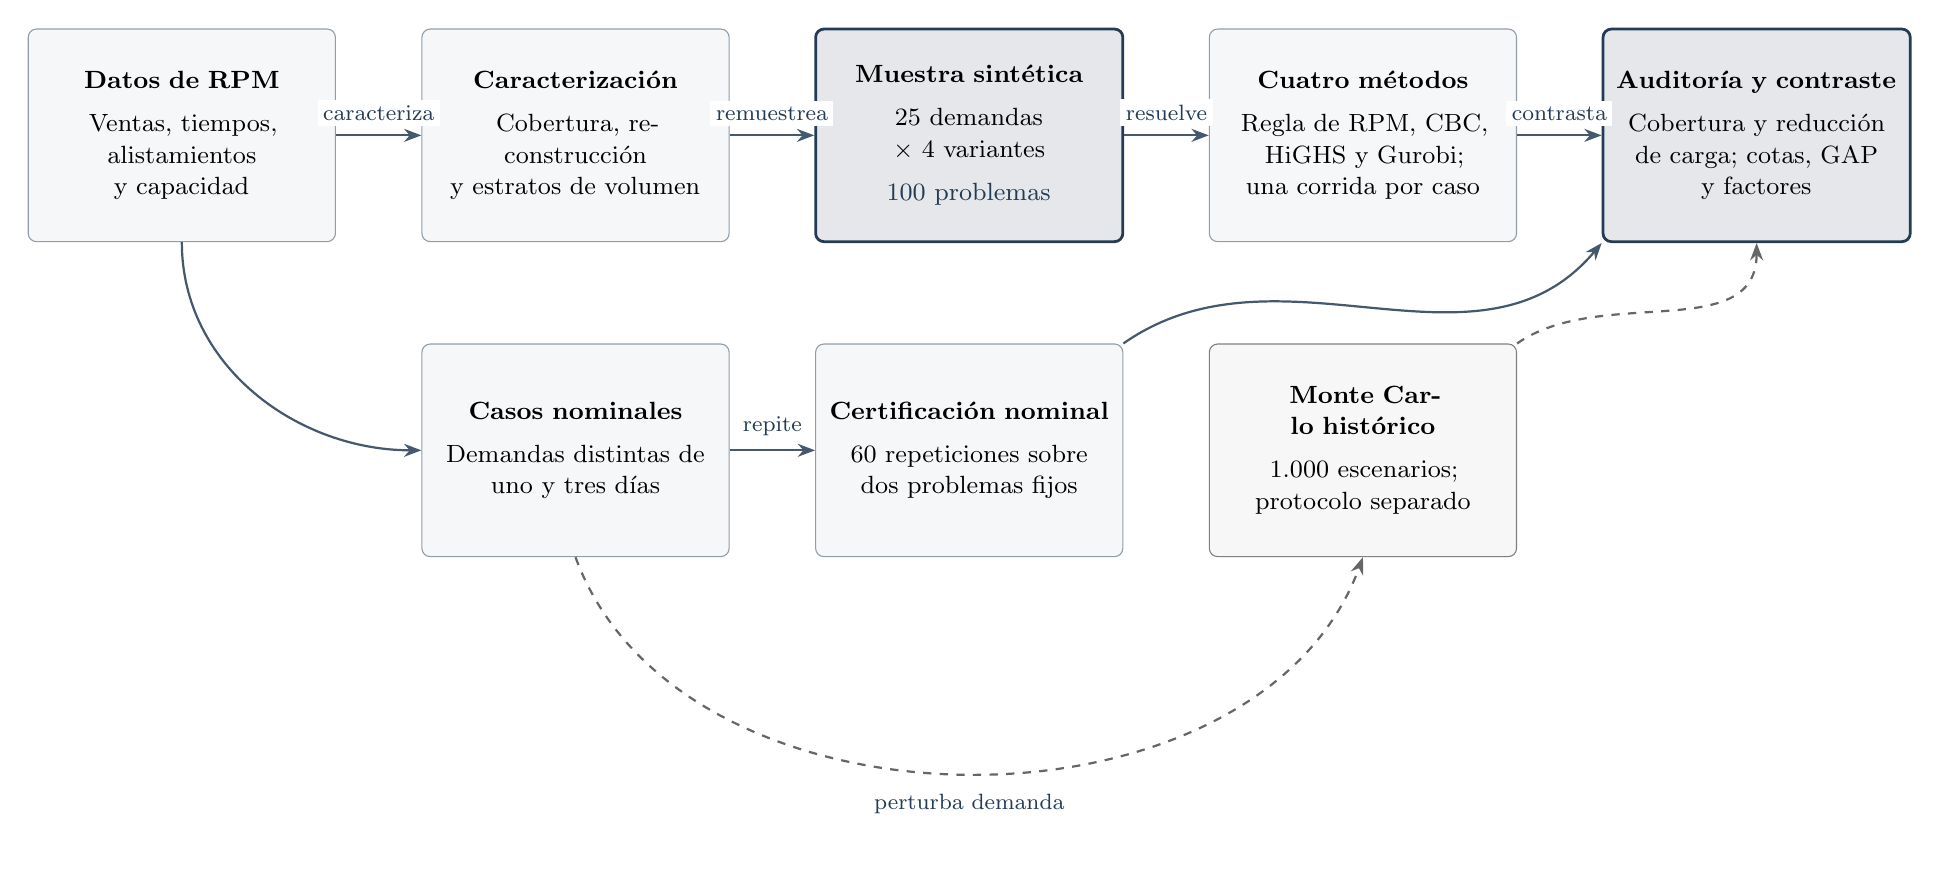
\begin{tikzpicture}[
 box/.style={draw=azul!50,rounded corners=3pt,fill=azul!4,align=center,text width=3.55cm,minimum height=2.7cm,inner sep=5pt,font=\fontsize{9.5}{11.5}\selectfont},
 core/.style={box,draw=azul,line width=1pt,fill=azul!12},
 flow/.style={-{Stealth[length=2.2mm]},line width=.8pt,draw=azul!85},
 aux/.style={flow,dashed,draw=black!60},
 lab/.style={font=\fontsize{8}{9}\selectfont,fill=white,inner sep=2pt,text=azul,align=center}]
\node[box] (data) at (0,4) {\textbf{Datos de RPM}\\[4pt]Ventas, tiempos,\\alistamientos y capacidad};
\node[box] (prep) at (5,4) {\textbf{Caracterización}\\[4pt]Cobertura, reconstrucción\\y estratos de volumen};
\node[core] (sample) at (10,4) {\textbf{Muestra sintética}\\[4pt]25 demandas $\times$ 4 variantes\\[4pt]\textcolor{azul}{100 problemas}};
\node[box] (methods) at (15,4) {\textbf{Cuatro métodos}\\[4pt]Regla de RPM, CBC,\\HiGHS y Gurobi;\\una corrida por caso};
\node[core] (report) at (20,4) {\textbf{Auditoría y contraste}\\[4pt]Cobertura y reducción\\de carga; cotas, GAP\\y factores};
\node[box] (nominal) at (5,0) {\textbf{Casos nominales}\\[4pt]Demandas distintas de\\uno y tres días};
\node[box] (cert) at (10,0) {\textbf{Certificación nominal}\\[4pt]60 repeticiones sobre\\dos problemas fijos};
\node[box,draw=black!50,fill=black!3] (mc) at (15,0) {\textbf{Monte Carlo histórico}\\[4pt]1.000 escenarios;\\protocolo separado};
\draw[flow] (data.east)--node[lab,above=3pt]{caracteriza} (prep.west);
\draw[flow] (prep.east)--node[lab,above=3pt]{remuestrea} (sample.west);
\draw[flow] (sample.east)--node[lab,above=3pt]{resuelve} (methods.west);
\draw[flow] (methods.east)--node[lab,above=3pt]{contrasta} (report.west);
\draw[flow] (data.south) to[out=-90,in=180] (nominal.west);
\draw[flow] (nominal.east)--node[lab,above=3pt]{repite} (cert.west);
\draw[flow] (cert.north east) to[out=35,in=230] (report.south west);
\draw[aux] (nominal.south) to[out=-70,in=-110] node[lab,below=5pt]{perturba demanda} (mc.south);
\draw[aux] (mc.north east) to[out=35,in=270] (report.south);
\end{tikzpicture}
\vspace{6mm}
\caption[Mapa metodológico del trabajo]{Mapa metodológico del trabajo. La ruta superior compara la regla de RPM y el MILP en cien problemas: 25 demandas con cuatro variantes cada una, 400 registros, mejora de carga y calidad de cotas. La ruta inferior conserva los dos casos nominales y el Monte Carlo histórico con sus protocolos propios.}
\label{fig:ruta_metodologica_rpm}
\fuente{elaboración propia a partir del procedimiento y las evidencias del trabajo}
\end{figure}
\end{landscape}

\subsection{Desarrollo de la ruta metodológica}
\textbf{Datos, preparación y caracterización.}
La caracterización registra la demanda, los tiempos de procesamiento, los alistamientos y la capacidad nominal. Los coeficientes observados se separan de los reconstruidos y se mantiene la precisión de cálculo y las unidades. La instancia queda descrita por la cobertura, la concentración de demanda y los agrupamientos; con estos no se fijan el horizonte ni se le adjudican familias al MILP. Lo que se obtiene en esta fase es una base de supuestos explícitos (véase la sección~\ref{sec:datos}).

\textbf{Referencia heurística.}
La implementación reproduce la regla de asignación de RPM y produce un plan para cada problema de la muestra. El registro conserva carga y demanda pendiente. La mejora porcentual compara planes que cubren idéntica demanda. La sección~\ref{sec:heuristica} explica la regla; las secciones~\ref{sec:resultados} y~\ref{sec:instancias} enlazan el caso nominal con las cien comparaciones.

\textbf{Asignación diaria y extensión multiperiodo.}
Para minimizar el trabajo de preparación y de procesamiento, respetando la capacidad de cada máquina y las demandas diarias, el MILP decide cuántas veces y en qué cantidad (enteras) activar la producción. Para cada lote, una cota superior permite deshacerse de horizontes de planificación demasiado pequeños, mientras que una solución factible prueba que el horizonte propuesto es suficiente (sección~\ref{sec:modelo}; la prueba del horizonte se da en la sección~\ref{sec:horizonte}). Las instancias nominales con horizonte de un y tres días satisfacen demandas distintas.

\Needspace{9\baselineskip}
\textbf{Resolución y certificación cruzada.}
Se comprueba demanda, capacidad, enlaces, integridad y objetivo. Un certificado del número de cotas cerrado se basa en el estado del motor y en el cierre de cotas; la brecha (GAP) cuantifica también qué de cerca están los planes factibles a la cota inferior. La muestra central incluye 100 problemas y 400 registros (una ejecución para cada uno de los cuatro métodos, sin inicio heredado) (véase Sección~\ref{sec:instancias}). Las 60 repeticiones nominales conservan este protocolo como una ilustración de la formulación (véanse Secciones~\ref{sec:resolucion} y~\ref{sec:resultados}).

\textbf{Sensibilidad y Monte Carlo histórico.}
A través de la sensibilidad se cuantifican los cambios en la demanda y la capacidad con el protocolo de certificación, el cual no presenta un límite interno. En el modelo de simulación de Monte Carlo se conservan 1.000 escenarios históricos, la distribución de la demanda, el presupuesto de resolución y la brecha residual. Es importante recordar que la simulación es una herramienta que permite resumir la variabilidad existente bajo los supuestos planteados \cite{law}. El hecho de contar con certificados nominales no afecta el estado de las corridas de simulación. En la sección \ref{sec:escenarios} se presentan los dos análisis y en el anexo \ref{an:historico} se identifican las fuentes.

\textbf{Aplicación, evidencia e interpretación.}
Esta aplicación también relaciona los registros con las asignaciones de carga, el cumplimiento y la evidencia de resolución. También permite la exportación tanto de los planes como de los indicadores identificados en cada instancia (\ref{sec:aplicacion}). El objetivo es una representación de la carga nominal de procesamiento y preparación; una posterior evaluación en planta puede permitir comparar el objetivo con los tiempos y costos efectivamente observados.


\clearpage
\subsection{Trazabilidad de las etapas y sus resultados}
La tabla~\ref{tab:trazabilidad_metodologica} relaciona las etapas del mapa con su desarrollo y su evidencia. La secuencia distingue preparación de datos, construcción de planes y comprobación de resultados.
\begin{table}[H]\centering\small
\caption{Etapas metodológicas, productos y ubicación de la evidencia}\label{tab:trazabilidad_metodologica}
\begin{tabular}{p{33mm}p{65mm}p{44mm}}\toprule
Etapa & Producto verificable & Desarrollo y respaldo\\\midrule
Datos y caracterización & Matrices nominales, cobertura observada y análisis de reconstrucción & Sección~\ref{sec:datos}; anexos~\ref{an:datos} y~\ref{an:construccion}\\[4pt]
Referencia heurística & Plan y cobertura de cada problema; carga en parejas completas & Secciones~\ref{sec:heuristica} y~\ref{sec:instancias}; anexo~\ref{an:heuristica}\\[4pt]
Asignación MILP & Cantidades, activaciones y carga de los planes completos & Secciones~\ref{sec:modelo} y~\ref{sec:instancias}\\[4pt]
Extensión multiperiodo & Plan de tres días y prueba del horizonte para el lote fijo & Apartado~\ref{sec:horizonte}; anexos~\ref{an:prueba} y~\ref{an:maestro}\\[4pt]
Certificación cruzada & 60 corridas nominales; estados, cotas y planes verificados & Sección~\ref{sec:resolucion}; anexos C e~\ref{an:desarrollo_complementario}\\[4pt]
Estudio de instancias & Cien problemas, cuatro métodos, reducción frente a la regla de RPM, GAP y perfil de factores & Sección~\ref{sec:instancias}; anexo~\ref{an:instancias100}\\[4pt]
Análisis histórico & Sensibilidad actual y 1.000 escenarios históricos con protocolos separados & Sección~\ref{sec:escenarios}; anexos~\ref{an:historico} y~\ref{an:desarrollo_complementario}\\[4pt]
Aplicación y evidencia & Consulta de indicadores y exportación de planes y registros & Sección~\ref{sec:aplicacion}; anexos E e~\ref{an:desarrollo_complementario}\\\bottomrule
\end{tabular}
\end{table}

\subsection{Fundamentos de la formulación}
Con la programación entera es posible incluir decisiones binarias y costos fijos por activación en un modelo lineal \cite{taha}. En este modelo se requiere de la activación de una preparación si una máquina va a fabricar una referencia. La asignación generalizada es el punto de partida para la inclusión de recursos, capacidades y decisiones \cite{cattrysse}; en este problema a los anterior se añaden las decisiones enteras y la activación por periodo.

Cuando se trata de planificar máquinas con alistamientos se puede distinguir entre la asignación de la carga y la secuencia de fabricación \cite{unlu}. Esta distinción marca el alcance del modelo: la carga es cuantificada, pero no se intenta programar un taller flexible completo. La utilización de la hoja de recursos permite obtener un alistamiento por máquina que puede ser utilizado para modelar una preparación fija pero no para realizar cálculos de cambios dependientes de la secuencia o del molde.

\subsection{Tipos de evidencia}
El informe separa los resultados de las instancias nominales de las conclusiones que surgen de los análisis de sensibilidad y de simulación. Los registros, las comprobaciones, los planes de ejecución, los parámetros y los valores de entrada de las 60 corridas nominales se han dejado sin alteraciones en el resultado de la ejecución del 25 de octubre de 2026 (26 de octubre UTC). Esta revisión compara las salidas de las corridas nominales con los registros de respaldo. Se describen en los anexos las fuentes de los análisis de Monte Carlo, imputación y agrupación históricos que siguen dentro del alcance del informe original. No se ha hecho nada para convertir el resultado de las dos instancias nominales en valores certificados a posteriori tras su finalización.

En cuanto a las unidades de análisis, las define la tabla~\ref{tab:instancias}. No es lo mismo multiplicar una demanda diaria por el número de días que alterar el horizonte con un lote fijo. De igual modo, al comparar uno y tres días se recurre a dos instancias concretas y no a la misma demanda distribuida en otras tantas ventanas.

\begin{table}[H]\centering\small
\caption{Instancias originales utilizadas en la validación}\label{tab:instancias}
\begin{tabular}{lrr}\toprule
Característica & Caso diario & Caso de tres días\\\midrule
Referencias con demanda positiva & 99 & 200\\
Máquinas & 10 & 10\\
Horizonte de la corrida (días) & 1 & 3\\
Demanda total (unidades) & 14.188 & 45.987\\
Pares producto--máquina & 990 & 2.000\\
Capacidad total (min) & 14.400 & 43.200\\
Repeticiones por optimizador & 10 & 10\\\bottomrule
\end{tabular}
\fuente{matrices C, D y S y protocolo de las corridas}
\end{table}

La revisión de antecedentes y su relación con el modelo figura en el anexo~\ref{an:desarrollo_complementario}.

\section{Datos, calidad y caracterización}\label{sec:datos}
\subsection{Tiempos nominales y cobertura}
Los minutos de procesamiento por unidad de la referencia $i$ en la máquina $j$ se denotan con $C_{ij}$, el tiempo de preparación con $S_j$ y la demanda con $D_i$. Se mantiene la exactitud de los coeficientes a efectos de resolver y comprobar; el redondeo queda para las tablas que se presenten. Un redondeo anticipado podría modificar la capacidad o las asignaciones, así como las mínimas diferencias de unas alternativas a otras.

En el caso de las 99 referencias diarias hay 990 combinaciones posibles, de las cuales 819 (un 82,73\%) cuentan con registros directos. Las 171 restantes requieren una hipótesis de tiempo o bien una restricción de compatibilidad justificada. Que no haya observación no es prueba de imposibilidad técnica, del mismo modo que un tiempo estimado no acredita que el par sea viable en la práctica.

La revisión hace una distinción entre dos matrices. Por un lado está la \textit{matriz nominal publicada}, la que se emplea en las certificaciones vigentes y los resultados principales. La \textit{matriz reconstruida} parte de los registros de origen a los que se han aplicado reglas explícitas de estimación y depuración. No son lo mismo: un repaso histórico ha dejado constancia de discrepancias en 174 celdas, 171 de pares sin observar y tres con registro. El método de imputación que dio mejor resultado en una validación posterior no se aplicó retrospectivamente a todos los coeficientes de la publicación.

\subsection{Evaluación de una regla de imputación}
Con la revalidación histórica se han cotejado cuatro estimadores (media global, por referencia y por máquina, así como el modelo aditivo) ocultando las observaciones. De las 100 particiones hechas, la media por máquina ha sido la opción más ventajosa en 96 de ellas con un MAE medio de 0,1888 min/unidad. Esto la hace idónea para aplicar como una regla reproducible de reconstrucción en la muestra, si bien no avala la precisión de las celdas que de entrada faltaban. Las discrepancias y los resúmenes correspondientes figuran en el anexo~\ref{an:datos}.

Respecto al plan nominal diario, 98 de los 99 pares activos cuentan con soporte directo. El otro par acumula 1.337 unidades, lo que supone un 9,42\% del volumen. La importancia de un dato que falta se mide por la producción que le corresponde y no únicamente por el tanto por ciento de celdas ausentes. Por ello, antes de poner en marcha dicho plan es necesario medir el par activo sin observación para verificar su compatibilidad.

\subsection{Concentración de demanda y grupos descriptivos}
La demanda de la instancia diaria se concentra en 28 de las 99 referencias, que por sí solas representan el 80\,\% del volumen. Conviene hacer la distinción entre un producto de gran volumen y una referencia de menor volumen dada esta estructura, no obstante, reservarles una máquina requiere un examen de la capacidad de la solución y del costo total antes de proceder.

\begin{figure}[H]\centering
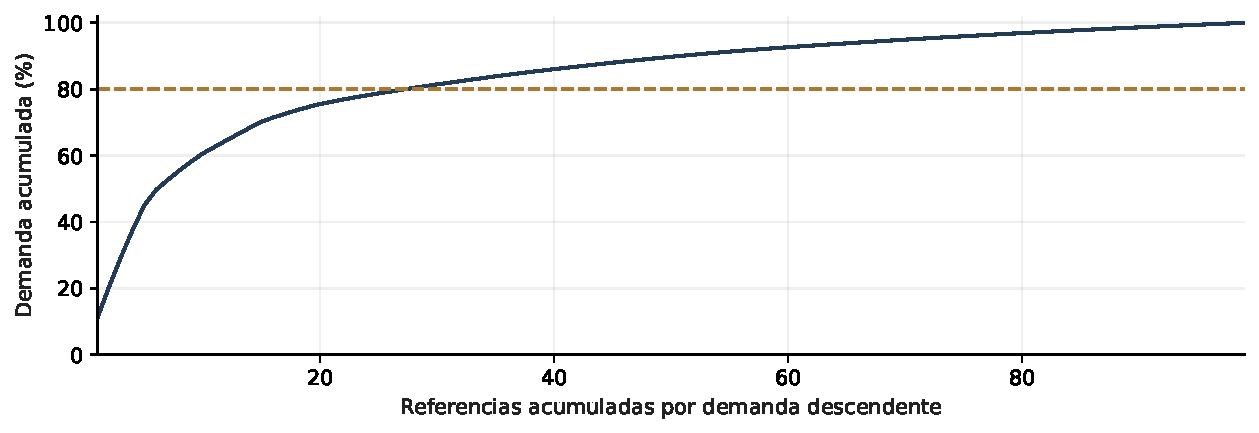
\includegraphics[width=.9\linewidth]{figuras/pareto.pdf}
\caption[Concentración de la demanda diaria]{Concentración de la demanda de la instancia diaria. La curva se recalculó con el vector de demanda certificado.}
\end{figure}

Para el análisis de los productos se han considerado la demanda, así como la variación de los tiempos entre máquinas. El coeficiente de Silhouette, el cual representa un resumen de los valores de cohesión y separación de los grupos \cite{rousseeuw}, ha preferido dos grupos de productos (0,709). Sin embargo, para una mayor interpretación, se han mantenido tres grupos, uno de baja escala (42 referencias), otro de rotación media (52 referencias), y el último de alto volumen (cinco referencias). Esto tiene un Silhouette de 0,555. Por tanto, se ha dado prioridad a una interpretación de los grupos más que al máximo permitido por el coeficiente.

Respecto a las máquinas, el análisis histórico basado en tres variables de desempeño arrojó grupos de 1, 1 y 8. Tanto K-Means como Ward han llegado a esa misma partición; este último es un método de agrupación jerárquico \cite{ward}. Que dos algoritmos coincidan con idénticos datos no constituye una validación externa ni da pie a considerar a los ocho equipos como intercambiables, pues sus preparaciones y tiempos son diferentes.

El número de grupos no se corresponde con el de días de producción. Los grupos describen patrones, mientras que el horizonte viene determinado por la demanda fija, las capacidades y si es viable trazar un plan. Por su parte, no se recurre a ensayos con las mismas variables que dieron lugar a los grupos para sostener causalidad o validar familias productivas independientes.

El anexo~\ref{an:desarrollo_complementario} documenta la construcción de los vectores y sus supuestos.

\section{Construcción de la referencia heurística}\label{sec:heuristica}
La caracterización describe las referencias y los recursos. La etapa heurística formaliza la regla de asignación utilizada como referencia en RPM y construye un plan reproducible para compararlo con el MILP. Ambos procedimientos utilizan la misma demanda, los mismos tiempos y las mismas capacidades. La diferencia de carga refleja las decisiones de asignación y activación dentro de esa instancia común.

\subsection{Regla de asignación y control de capacidad}
La heurística se encarga de ordenar las referencias en función de la demanda, de mayor a menor. En el caso de cada referencia, se recorre a las máquinas por tiempo unitario, de menor a mayor, y se le adjudican las unidades que su capacidad residual depara, con el descuento del alistamiento si se pone en marcha el par. Si quedan unidades pendientes, la heurística continúa con la máquina siguiente; cuando cubre la demanda de la referencia, pasa a la siguiente referencia. El anexo~\ref{an:heuristica} detalla tanto el algoritmo como la forma de resolver empates.

El algoritmo contempla el número de productos, la activación, la carga y los productos faltantes. Sin embargo, un producto de lote particular elegido como producto rápido podría no satisfacer todas las necesidades de productos del lote. Podría estar utilizando una capacidad que sería útil para otro producto, o podría estar desparramando la producción, en contra de la concentración de la producción para un producto que el MILP habría hecho para evitar una preparación. Debido a estas interacciones, se hace necesario comparar la heurística con una solución de optimización de conjunto.

\subsection{Producto de la etapa y criterio de comparación}
Con la regla aplicada diariamente tenemos 13.684 minutos de carga, sin faltantes. En el plan se incluye entonces la referencia RPM para este lote. El plan no asigna fechas ni decisiones a los individuos que no estaban en el archivo histórico. Para poder realizar la comparación porcentual es necesario que el plan formal y el plan heurístico incluyan las mismas unidades. Si la heurística no atiende toda la demanda, en el análisis se incluye esta información y se conserva el porcentaje de reducción para las unidades en las que se pudo armar pareja.

Una vez calculada esta referencia, la sección~\ref{sec:modelo} se encarga de plantear la decisión conjunta. En la sección~\ref{sec:resultados} contrasta los planes obtenidos mediante la heurística y el modelo MILP, y examina las
reasignaciones que explican las diferencias en la carga agregada de producción.

\section{Asignación MILP diaria y extensión multiperiodo}\label{sec:modelo}
En la ruta de comparación en el mapa usamos una misma fórmula para los casos de uno, tres y cinco días. Los ejemplos del caso de un día y tres días son representativos de cómo se extiende la asignación para el horizonte multiperiodo. Para una misma cantidad en el lote, mantenemos la demanda, los tiempos unitarios, los alistamientos y capacidades de las máquinas por día. Con el índice tiempo, se incluye el número de días en el horizonte, pero la demanda no es función del número de días.

\subsection{Conjuntos, parámetros y variables}
Con $I$ y $J$ como conjuntos de referencias y de máquinas y tomando a $T_H=\{1,\ldots,H\}$ como los días del horizonte. La demanda $D_i$ corresponde a la del lote que debe completarse en el periodo. Como datos de entrada el modelo tiene $C_{ij}>0$, $S_j\geq0$ y la capacidad $K_{jt}>0$, siendo esta última de 1.440 minutos en las instancias evaluadas. Las unidades producidas se representan por $x_{ijt}\in\mathbb Z_{\geq0}$ y $y_{ijt}\in\{0,1\}$ indica si una preparación está o no activada. De la capacidad y la demanda se obtiene la cota de enlace:
\begin{equation}
U_{ijt}=\max\left\{0,\min\left[D_i,\left\lfloor\frac{K_{jt}-S_j}{C_{ij}}\right\rfloor\right]\right\}.
\label{eq:U}
\end{equation}
Al ser $U_{ijt}=0$, la combinación de que se trata no es idónea para producir una unidad con la capacidad y preparación exigidas. El modelo respalda tal restricción con sus supuestos, si bien no en el sentido más estricto cuando se tienen presentes las interacciones de las referencias.

\subsection{Modelo de asignación para un horizonte fijo}
\begin{align}
\min\quad Z_H &=\sum_{t\in T_H}\sum_{j\in J}\sum_{i\in I}(C_{ij}x_{ijt}+S_jy_{ijt}) \label{eq:obj}\\
\text{sujeto a}\quad
\sum_{t\in T_H}\sum_{j\in J}x_{ijt}&=D_i && i\in I, \label{eq:dem}\\
\sum_{i\in I}(C_{ij}x_{ijt}+S_jy_{ijt})&\leq K_{jt} &&j\in J,\ t\in T_H, \label{eq:cap}\\
x_{ijt}&\leq U_{ijt}y_{ijt} &&i\in I,\ j\in J,\ t\in T_H, \label{eq:link}\\
x_{ijt}&\in\mathbb Z_{\geq0},\quad y_{ijt}\in\{0,1\}.\label{eq:dom}
\end{align}
Con la ecuación~\eqref{eq:dem} se hace necesario cubrir con exactitud la demanda de cada referencia, algo que un porcentaje de cobertura general no está en condiciones de ofrecer. La ecuación~\eqref{eq:cap} reúne el procesamiento y la preparación bajo un mismo presupuesto de capacidad. La ecuación~\eqref{eq:link} exige activar el par cuando existe producción. De haber una preparación positiva, una activación carente de unidades no aporta al objetivo y se puede descartar sin menoscabo de la factibilidad.

Al poner $H=1$ se tiene el caso de cada día. Para una referencia con demanda positiva la desigualdad $\sum_{j,t}y_{ijt}\geq1$ es de aplicación; esto refuerza la relajación sin apartar las soluciones enteras que sean factibles. La diferencia entre las 1.099 restricciones de la formulación diaria de base y las 1.198 filas del modelo resuelto se debe a los 99 cortes de cobertura.

$Z_H$ representa la suma de minutos de ocupación en distintas máquinas, no el tiempo transcurrido hasta cerrar la última orden ni un gasto en dinero. Hay que tener en cuenta que minimizar la carga total no es lo mismo que equilibrar la utilización, pues la solución podría volcar la producción a los equipos más eficientes y dejar holgura en los demás. La carga máxima se da como dato descriptivo, no como un makespan optimizado.

\subsection{Tamaño y alcance de la formulación}
La formulación diaria contiene 990 variables enteras de cantidad y 990 binarias, sin que haya variables continuas de decisión. Si se toman 200 referencias, diez máquinas y un periodo de tres días, la representación en su forma totalmente desagregada pasa a tener 6.000 variables de cantidad y otras tantas binarias. La formulación de base incluye 200 igualdades de demanda, 30 desigualdades de capacidad y 6.000 enlaces, lo que suma 6.230 restricciones antes de aplicar refuerzos.

No hay que confundir estos conteos de concepto con el tamaño del maestro selectivo empleado en las corridas nominales documentadas. Para el caso de los tres días, el maestro final que se registra consta de 5.200 variables y 10.924 restricciones. El hecho de reducir las variables va de la mano con el fortalecimiento de las restricciones; no es automático que un número inferior de columnas signifique menos filas ni se puede inferir de ello el tiempo de cálculo.
% !TeX root = ../Trabajo_RPM.tex
\subsection{Interpretación económica y dimensional}
La función objetivo asigna el mismo peso a un minuto en cualquier máquina y mide la carga agregada de trabajo. No incorpora diferencias de consumo eléctrico, personal o tarifas entre equipos. En el caso de añadir costos por minuto el objetivo adquiriría un carácter monetario y los coeficientes se verían alterados; los óptimos que se dan no son directamente interpretables bajo ese nuevo objetivo.

Como nota, dividir lotes permite economías de procesamiento, ya que se pueden utilizar máquinas de mayor velocidad, pero se suele realizar a costa de un mayor número de activaciones. Esto se refleja en el modelo por $C_{ij}x_{ijt}+S_jy_{ijt}$. No se trata de tener siete productos cuando tenemos 207 activaciones en tres días con 200 referencias, una sola referencia puede provocar que tengamos más de una activación extra. El número de referencias activadas varias veces y el número de referencias activadas en varias máquinas se da en la Sección~\ref{sec:resultados}.
Por otro lado, la restricción de capacidad es local. Es necesario que se cumpla $Z_H\leq\sum_{j,t}K_{jt}$ pero no es suficiente. Podríamos sobrepasar la capacidad de una de las máquinas aunque no nos pasemos en el resto de las máquinas. Por esta razón se considera cada combinación máquina y día en lugar del promedio de utilización. En cierto sentido, esta propiedad es la que complica el problema y por este motivo se ha de verificar la distribución temporal del maestro agregado.

\subsection{Por qué importa la cota de enlace}
Al relajar el problema, la restricción $x_{ijt}\leq M y_{ijt}$ implica que la variable $y_{ijt}$ debe cumplir $y_{ijt}\geq x_{ijt}/M$. Si $M$ es grande se puede disminuir el valor de $y_{ijt}$ hasta ese valor fraccionario y únicamente se pagaría $S_jx_{ijt}/M$ por la preparación si se puede hacer cumpliendo con el resto de las restricciones. Sin embargo, en el problema entero, si hay producción, se debe tener el valor completo de $y_{ijt}$. Esta diferencia puede implicar que se tenga una peor cota inferior, pero no cambia el óptimo entero.

La cota mostrada en la ecuación~\eqref{eq:U} se obtiene utilizando dos restricciones que deben ser cumplidas por cualquier solución factible: no puede producirse más de lo que se demanda, y no puede utilizarse más de la capacidad disponible una vez hecha la preparación. Esto mantiene el conjunto de soluciones enteras del modelo original, y no se han hecho cambios como el modificar los tiempos ni el redondear la demanda para hacer más fácil la prueba. La variable entera no puede tomar valores mayores que la capacidad (que en el problema relajado es fraccionaria) de unidades, por eso se impone el piso.

El corte de cobertura viene a completar el enlace. Si bien la igualdad de la demanda y los enlaces obligan a tener al menos una activación en una solución entera donde $D_i>0$, la relajación admite activaciones fraccionarias repartidas entre varios pares. La condición $\sum_{j,t}y_{ijt}\geq1$ evita que se pague menos de una activación total por referencia. La mejora de la cota depende de la interacción entre los refuerzos; con los datos del experimento no se puede cuantificar su efecto por separado.

\subsection{Orden de las decisiones de horizonte y carga}
Reducir el tiempo agregado y localizar el horizonte más pequeño son dos objetivos distintos. El método para avanzar es una regla de tipo lexicográfico: se fija $H^*$, en la medida de lo posible, y luego se minimiza $Z_{H^*}$. No es cuestión de sumar un día y un minuto con pesos arbitrarios. Un horizonte mayor puede reducir la carga agregada, aunque deje de ser el menor plazo posible en días.

Dadas unas reglas de alistamiento y una capacidad diaria que se va repitiendo, todo plan viable de $H$ días puede extenderse a $H+1$ con el último exento de producción. De ello se deduce que $\mathcal F_H\subseteq\mathcal F_{H+1}$ si se asocia cada plan con su nula extensión de producción en el día de más, y que $Z_{H+1}^*\leq Z_H^*$. Esta propiedad parte del supuesto de que al ensanchar la ventana no se introducen nuevas demandas o restricciones, aunque no por ello se garantiza un descenso estricto del objetivo.

Si se quiere analizar una ventana más amplia que la ventana mínima demostrada, entonces, debe resolverse el modelo con el tamaño deseado de la ventana, pero manteniendo la misma demanda fija. En este caso, el certificado de carga es para la ventana analizada, y la prueba para el mínimo de días es la prueba de factibilidad. El horizonte automático es el que se utiliza en la versión de la aplicación descrita en este trabajo. La propiedad enunciada anteriormente es de la formulación y no es que la aplicación necesariamente tenga un selector del horizonte manualmente.

\subsection{Justificación del horizonte de tres días}\label{sec:horizonte}
La calibración descrita en el anexo~\ref{an:construccion} ha establecido el lote multiperiodo con un factor de 3. Una vez que se han fijado las 45.987 unidades, se mantiene el vector de demandas y se busca el menor horizonte de tiempo posible. La prueba no estima un horizonte de tiempo a partir de un vector de pedidos no relacionado con la construcción del lote. Para un vector de demanda fijo se define el horizonte mínimo por
\begin{equation}
	H^*=\min\{H\in\mathbb Z_{\geq1}:\mathcal F_H(D)\neq\varnothing\},
	\label{eq:hmin}
\end{equation}
donde $\mathcal F_H(D)$ representa el conjunto de planes factibles para un vector de demanda fijo $D$ y un horizonte de tiempo de $H$ días. Esto significa que en primer lugar se determina el menor horizonte de tiempo factible, y una vez determinado, se minimiza la carga de trabajo para dicho horizonte. Así, que un plan haya resultado óptimo para un horizonte de 3 días no implica que sea un plan óptimo para un horizonte de 2 días.
En el caso del lote de 200 referencias y 45.987 unidades se establece una cota inferior en la carga de trabajo,
\begin{equation}
	L(D)=\sum_{i\in I}D_i\min_{j\in J}C_{ij}
	+ |I^+|\min_{j\in J}S_j,
	\label{eq:cotaH}
\end{equation}
donde $I^+=\{i:D_i>0\}$. Cada unidad debe ser producida, como mínimo, en el menor tiempo unitario posible de su referencia, y cada referencia con demanda positiva debe ser preparada al menos una vez. Por tanto, la cota inferior está dada por la suma de elecciones optimistas sin requerir que sean alcanzables dentro de una misma asignación factible. La cota inferior permite obtener una condición necesaria sobre la capacidad, pero no un plan de producción.

El cálculo con las matrices conservadas produce
\begin{equation}
L(D)=29.748,4944\ \text{min}>2(10)(1.440)=28.800\ \text{min}.
\end{equation}
La carga mínima supera la capacidad de uno y dos días. El plan certificado demuestra factibilidad en tres. Ambas evidencias establecen $H^*=3$ para este lote y estos parámetros. El resultado depende de las cantidades, los tiempos y la capacidad; no del número de clusters ni únicamente de las 200 referencias. Un cambio en los datos exige repetir la prueba.

El hecho de que en el pasado se haya obtenido factibilidad en dos días con 30.656 unidades no va en contra de lo demostrado aquí, pues se empleaba otro lote. El vector de esta demostración da un total de 45.987 unidades. La demanda no se mueve en una búsqueda de horizonte; hacerla proporcional al número de días de cuenta sería alterar el problema a resolver.

\section{Estrategia de resolución y certificación}\label{sec:resolucion}
\subsection{Cotas, relajación y criterio numérico}
Con el fin de minimizar, una solución factible e íntegra da lugar a una cota superior $UB$, en tanto que la relajación o el trabajo del solver ofrece una cota inferior $LB$. El óptimo se sujeta a $LB\leq Z_H^*\leq UB$. En el caso de $UB>0$, la brecha relativa se formula de la siguiente manera:
\begin{equation}
g=100\frac{\max\{0,UB-LB\}}{|UB|}.
\end{equation}
Para evitar las mínimas brechas negativas que la aritmética de punto flotante puede originar, se recurre al máximo con cero; también se mantiene la magnitud $|UB-LB|$ a fin de comprobar el cierre. Que un GAP se muestre como 0,00\% por redondeo no basta para atestiguar la optimalidad.

En las nuevas corridas se pide un GAP relativo y absoluto de cero sin poner límite interno de tiempo. Si bien CBC hace uso de ramificación y cortes \cite{cbc}, HiGHS y Gurobi tienen parámetros distintos para cada una de las dos brechas \cite{highs,gurobi}. Tal configuración obliga a proseguir con la prueba, pero no asegura una duración finita en la práctica ni quita las tolerancias de factibilidad, integralidad o precisión numérica. Quitar el límite del optimizador no hace desaparecer los externos de la infraestructura.

Se dice que una corrida es buena cuando el estado nativo respalda la optimalidad de la corrida, cuando la corrida satisface cotas coherentes, y cuando el plan entero satisface la verificación dentro de una tolerancia de $10^{-5}$. Nuestros certificados son de naturaleza numérica; no es posible tener una prueba formal de la aritmética racional, o una certificación independiente de la implementación del solver.

\subsection{Fortalecimiento y desagregación selectiva}
La cota de enlace de la Ecuaci{\'o}n~\eqref{eq:U} cumple su funci{\'o}n, porque evita el uso de constantes de magnitud artificial. La formulación MILP mantiene esta cota de enlace durante el proceso de resolución. Para el horizonte de tres d{\'i}as, se describe en los registros un procedimiento de desagregaci{\'o}n selectiva con poda lagrangiana: se resuelve un maestro agregado y se comprueba si sus asignaciones se distribuyen en el tiempo de manera factible para cada d{\'i}a; si no es el caso, se desagregan las m{\'a}quinas que corresponda.

El maestro agregado arroja una cota de 34.131 minutos, que no es el {\'o}ptimo del modelo multiperiodo completo. El subproblema es incapaz de distribuir la asignaci{\'o}n de M1. Con M1 desagregada, el maestro arroja una cota de 34.132 minutos. Dentro del margen de tolerancia, la cota se ajusta a la del {\'o}ptimo de un plan completo que respete las capacidades d{\'i}a por d{\'i}a, m{\'a}quina por m{\'a}quina. La igualdad de la cota con el plan verificado permite cerrar la brecha para esta instancia. En los anexos~\ref{an:prueba} y~\ref{an:maestro} se detallan la prueba, el maestro, la distribuci{\'o}n y la decisi{\'o}n de poda.

La poda descrita en los registros usa programaci\'{o}n din\'{a}mica \cite{taha} y una cota lagrangiana para fijar a cero 579 de los 2.000 pares del agregado. Esta acci{\'o}n es leg{\'i}tima si la cota condicional excluye toda posibilidad de mejora de la soluci{\'o}n factible, dados los errores de redondeo. No se trata de eliminar pares que sean lentos. En los registros y en los rastros del c{\'o}digo queda documentada la implementaci{\'o}n que se ha usado. La auditor{\'i}a en la revisi{\'o}n respalda las cotas, los planes y las salidas, pero no sustituye la demostraci{\'o}n formal del c{\'o}digo de poda.

\subsection{Protocolo nominal de referencia}
Mantener diez repeticiones por horizonte y solver con una semilla del 42 al 51 y un solo hilo de trabajo, variando el orden de los solvers en cada repetición. En los dos casos ejemplo. La trazabilidad de esta ejecución es: Python 3.14.9, PuLP 3.3.0, HiGHS 1.15.1, Gurobi 13.0.3 y CBC Devel (usando cbcbox 2.924). Nótese que no es CBC 2.10.3 que algunas distribuciones de PuLP tienen. El log ha sido tomado de una máquina Linux x86\_64 con 16 CPU lógicas disponibles. No se referencia el modelo específico de procesador en el log.

Todos los solvers han empezado con la misma solución factible para cada horizonte. En el caso de un día, dicha solución factible proviene de una heurística determinista con valor 13.684 minutos. En el caso de tres días, se ha tomado una solución factible previamente encontrada por HiGHS que coincide con la solución certificada. La solución factible inicial se provee como cota superior para todos los solvers. Cada solver debe encontrar su propia cota inferior y realizar su propia prueba de cierre. El tiempo usado en las repeticiones no está contaminado por el tiempo requerido previamente para encontrar la solución factible.

Las diez repeticiones son en la misma instancia, pero con diferentes semillas y ambientes. No son diez muestras independientes de demanda. Las semillas no resultan en una trayectoria aleatoria con la misma característica entre los diversos solvers. Este protocolo estandarizado es para poder registrar los resultados de estabilidad y tiempo, no para establecer un ranking universal de solvers o para generalizar a otras instancias.

En el anexo~\ref{an:desarrollo_complementario} se describen las pruebas numéricas de certificación.

\section{Resultados nominales y certificación cruzada}\label{sec:resultados}
En esta sección se muestran los resultados para dos casos estables y sus certificados. En la Sección~\ref{sec:instancias} se muestra la comparación más relevante, sobre variedad de instancias. Los resultados para los estados y tiempos de los certificados no se confunden con los de las repeticiones nominales.
En esta sección se muestran los resultados para los dos casos mencionados, plan diario y multiperiodo. Se muestran los resultados para las cantidades, el tiempo de preparación y la carga en máquinas. Luego se comparan los resultados para la certificación con los tres motores. La comparación que se hace en esta sección con la heurística es para el caso diario, considerando la misma cobertura de la demanda. Los resultados para 100 problemas se muestran en la Sección~\ref{sec:instancias}.

\subsection{Plan diario}
El valor certificado para 99 referencias es
\begin{equation}
Z_1^*=11.547,4126=9.147,2106+2.400,2020\ \text{min},
\end{equation}
El primer sumando se debe al procesamiento y el segundo a la preparación. Con 99 pares activos el plan da cobertura a las 14.188 unidades. No hay ninguna referencia que se parta entre más de una máquina en el plan conservado, algo que viene dado por la solución y no por una restricción del modelo. En cuanto a la ocupación global, es un 80,2\% de los 14.400 minutos de los que se dispone, mientras que la holgura total es de 2.852,5874 minutos. Los alistamientos representan el 20,79\% del objetivo. La figura~\ref{fig:diario} hace la distinción entre los dos componentes para cada máquina.

\begin{figure}[H]\centering
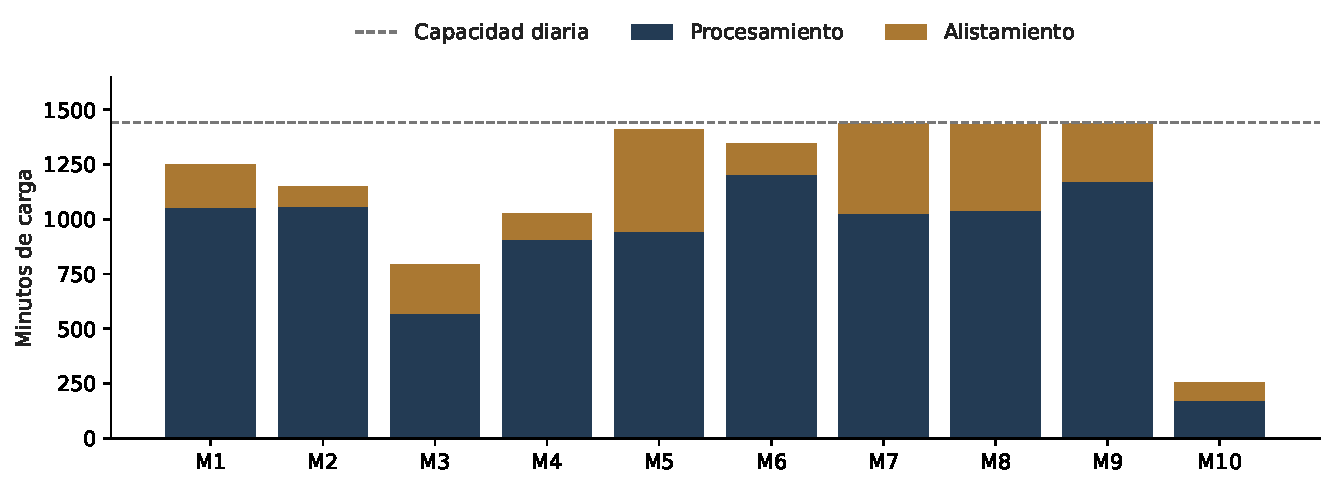
\includegraphics[width=\linewidth]{figuras/carga_diaria.pdf}
\caption[Carga diaria por máquina]{Carga del plan diario certificado, con separación de procesamiento y preparación.}\label{fig:diario}
\fuente{plan CBC, repetición 1; cálculo directo con C y S}
\end{figure}

M7, M8 y M9 están a punto de su capacidad diaria. El resto de las máquinas tienen un margen amplio, M10 sobre todo. Pero esa holgura no debe tomarse como capacidad que se pueda cambiar de una a otra con facilidad: mover un producto podría encarecer el tiempo unitario, hacer falta una preparación o exigir una compatibilidad por confirmar. De la forma en que se usan tampoco se extrae ningún consejo para desinvertir en equipos.

La referencia heurística de la sección~\ref{sec:heuristica} atiende el mismo lote sin faltantes. La mejora nominal es
\begin{equation}
R=100\frac{13.684,4886-11.547,4126}{13.684,4886}=15,6168\%.
\end{equation}
Los 2.137 minutos de diferencia corresponden a carga nominal evitada frente a la heurística. No se trata de una rebaja del plazo calendario ni de un ahorro real que se haya cuantificado en un ensayo de planta. La comparación tiene su validez en que los dos planes cubren el mismo lote y se rigen por las mismas normas.

\begin{table}[H]\centering\small
\caption{Cambios de asignación que ilustran la mejora diaria}
\begin{tabular}{p{51mm}p{35mm}p{24mm}r}\toprule
Referencia abreviada & Heurística: máquina/unidades & MILP & Reducción (min)\\\midrule
Envase 1000 PET Capri nuevo, 31 g & M1/145; M2/502 & M6/647 & 120,1660\\
Tapa negra EGO GEL 500 ml & M5/21; M10/21 & M5/42 & 83,7983\\
Conjunto base LZC limón 450 g & M2/68 & M7/68 & 78,3678\\\bottomrule
\end{tabular}
\fuente{heurística reconstruida y plan CBC diario, repetición 1; identificadores completos en el CSV de respaldo}
\end{table}
El primer cambio concentra 647 unidades en M6 y evita repartirlas entre M1 y M2. El segundo elimina una preparación en M10. Son contribuciones individuales al ahorro conjunto; otras referencias pueden aumentar su carga para liberar capacidad donde produce más beneficio.

\subsection{Plan de tres días}
El valor actualizado para 200 referencias es
\begin{equation}
Z_3^*=34.132,1434=28.663,9914+5.468,1520\ \text{min}.
\end{equation}
Se cumplen las 45.987 unidades y todas las capacidades máquina--día. La ocupación agregada es del 79,01\% de 43.200 minutos y la holgura total es de 9.067,8566 minutos. La preparación equivale al 16,02\% del objetivo. El plan exportado registra 207 activaciones producto--máquina--día para 200 referencias: en el plan CBC, repetición 1, cinco referencias tienen varias activaciones y cuatro utilizan varias máquinas. Los dos conteos describen propiedades distintas: una referencia puede activar la misma máquina en días diferentes. La figura~\ref{fig:tres} muestra la carga desagregada del plan de referencia.

\begin{figure}[H]\centering
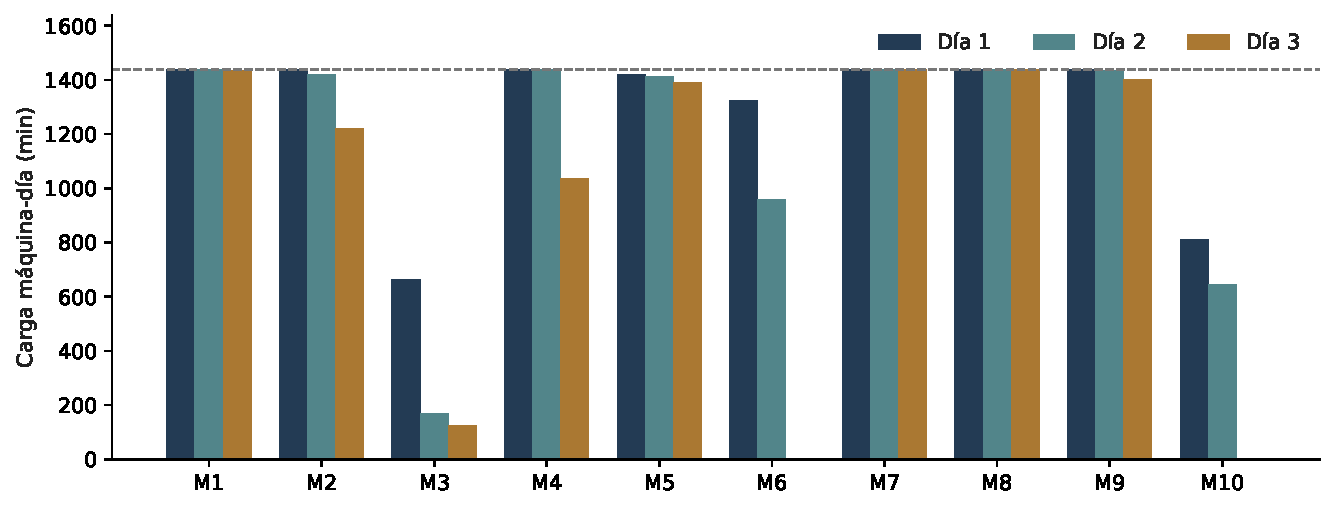
\includegraphics[width=\linewidth]{figuras/carga_tres_dias.pdf}
\caption[Carga por máquina y día]{Distribución diaria de la carga en un plan certificado de tres días.}\label{fig:tres}
\fuente{plan CBC, repetición 1; activaciones reconstruidas a partir de producción positiva}
\end{figure}

El estudio en su versión anterior se ceñía a un plan de 34.234,8717 minutos con una brecha positiva y factible. La nueva evidencia ha venido a sustituirlo como valor nominal de referencia; la reducción se sitúa en 102,7283 minutos, o sea el 0,3001\% del incumbente previo. Lo que más destaca del cambio es la verificación de todo el plan y el cierre de cotas. De todas formas, lo anterior queda documentado como un antecedente histórico, no como un fracaso en la certificación del resultado de hoy.

Los porcentajes de ocupación agregados no van en contra de la necesidad de tres días. La cota inferior de carga de 29.748 minutos supera los 28.800 minutos disponibles en dos días y demuestra su inviabilidad; el tercero aporta 14.400 minutos. Incluso con el horizonte mínimo acreditado, las unidades indivisibles, los alistamientos y las capacidades locales pueden dar lugar a holguras.

% !TeX root = ../Trabajo_RPM.tex
\subsection{Indicadores para interpretar el plan}
El trabajo define la ocupación de una máquina en un día como $L_{jt}=\sum_i(C_{ij}x_{ijt}+S_jy_{ijt})$. A partir de esta se calculan utilización $u_{jt}=100L_{jt}/K_{jt}$ y holgura $h_{jt}=K_{jt}-L_{jt}$. Para resumir el sistema se utiliza una razón de sumas:
\begin{equation}
u_{\mathrm{global}}=100\frac{\sum_{j,t}L_{jt}}{\sum_{j,t}K_{jt}}.
\end{equation}
Con esta expresión se pondera cada recurso en función de su capacidad. La media simple de utilizaciones coincide con esa razón cuando las capacidades son iguales, como ocurre en las instancias nominales. La razón de sumas mantiene la interpretación cuando los recursos tienen disponibilidades distintas.

La proporción de preparación viene dada por $p_S=100\sum_{i,j,t}S_jy_{ijt}/Z_H$. Que baje del caso diario al de tres días no acredita una mejora debida a la ampliación del horizonte, pues el volumen del lote y el conjunto de referencias también varían. El indicador describe la composición de cada objetivo; para un experimento causal del horizonte haría falta tener la demanda inalterable.

Para comprobar el cumplimiento se ha de recurrir a $r_i=\sum_{j,t}x_{ijt}-D_i$ como referencia. De lo contrario un total producido equivalente al pedido podría disimular un excedente en una referencia y un vacío en otra. De los 60 planes analizados el máximo de $|r_i|$ es cero, lo que tiene más valor como comprobación que un agregado del 100\,\% en toda regla.

El tablero debe dar a conocer el horizonte y la demanda total así como el estado frente al objetivo. Unos minutos sin contexto no informan de si se está ante un caso diario o multiperiodo, o bien una solución provisional. El valor de los indicadores reside en su vínculo con la instancia, no en acumular tarjetas en la interfaz.

\subsection{Implicaciones operativas de los resultados}
Con la asignación de cada día se concentra la carga en los equipos más eficientes, de modo que al resto le queda capacidad de sobra. Para que esa holgura pueda hacer las veces de reserva operativa hay que conocer qué referencias son de transferir y el coste en procesamiento y preparación extra que conlleva el cambio. El agregado óptimo es un buen punto de referencia, pero no constituye por sí mismo una política de contingencia.

La reducción nominal de 2.137 minutos frente a la heurística permite dar prioridad a una prueba de implementación. Lo recomendable es que un piloto mida lo que resta de tal diferencia una vez que se han considerado la disponibilidad del personal, las paradas y los cambios de preparación de los que se ha hecho cargo. Si la secuencia modifica los alistamientos, el asunto ya no es una simple actualización del certificado sino un problema de programación pormenorizada.

En tres días el resultado deja ver la diferencia entre una decisión de capacidad y otra de eficiencia. La cota muestra que el lote no cabe en dos días con los supuestos nominales, así que el modelo de carga se inclina por una distribución eficiente en un periodo de tres. Si se quisiera reducir a dos días habría que cambiar la demanda, la tecnología o la capacidad y resolver una nueva instancia con todos sus costos y restricciones.


\subsection{Certificación cruzada con CBC, HiGHS y Gurobi}\label{sec:comparacion}
Con la corrida de verificación del 25 de octubre de 2026 (26 de octubre en UTC) se dan por actualizadas las duraciones del experimento nominal. Los datos, las demandas y las capacidades se mantienen inalterados; el viejo expediente queda archivado y sus tiempos no se confunden con los de esta muestra.

Las 60 corridas quedan registradas en óptimo y pasan la prueba de factibilidad. En el horizonte diario de las treinta, el objetivo es 11.547 minutos; las otras treinta, de tres días, coinciden en 34.132 minutos. No se aprecia variación de calado en el valor de un motor respecto al otro. La comparación versa sobre el esfuerzo que hace falta para certificar y conseguir ese valor de acuerdo con lo que marca el protocolo.

\begin{table}[H]\centering\small
\caption{Tiempo total por corrida y frecuencia de certificación}\label{tab:tiempos}
\begin{tabular}{clrrrr}\toprule
Días & Motor & Certificadas & Media (s) & DE (s) & Rango (s)\\\midrule
1 & CBC & 10/10 & 13,529 & 0,665 & 12,824--14,746 \\
1 & Gurobi & 10/10 & 1,296 & 0,212 & 1,061--1,719 \\
1 & HiGHS & 10/10 & 6,824 & 1,030 & 5,900--9,480 \\
3 & CBC & 10/10 & 49,230 & 16,056 & 28,745--69,427 \\
3 & Gurobi & 10/10 & 9,614 & 0,156 & 9,428--9,972 \\
3 & HiGHS & 10/10 & 28,555 & 2,130 & 25,216--31,692 \\
\bottomrule\end{tabular}
\fuente{corrida del 25 de octubre de 2026, hora de Colombia; diez repeticiones por fila; DE muestral; tiempo total registrado por la aplicación}
\par\smallskip\begin{minipage}{.96\linewidth}\footnotesize
\textit{Nota:} las corridas de tres días empiezan del mismo plan que el obtenido antes con HiGHS, donde el objetivo es idéntico al óptimo confirmado. Los tiempos omiten la obtención previa de ese inicio. Cada motor lleva a cabo su propia prueba de cierre de cotas.
\end{minipage}
\end{table}

El mejor valor medio es el que se encontró utilizando Gurobi, seguido de HiGHS y después de CBC. La relación de las medias de CBC a Gurobi es de aproximadamente 5,12 en un periodo de tres días y la de HiGHS a Gurobi es de 2,97, cifras que si bien describen el experimento realizado no constituyen una estimación de aceleraciones garantizadas que fuesen válidas para cualquier otra formulación, máquina o versión. En lo que respecta a la dispersión de CBC en tres días, es la mayor de los demás motores: el máximo de sus diez ejecuciones fue de 69,427 s, cosa que no impidió cerrar la distancia que ha separado tal motor de Gurobi.

\begin{figure}[H]\centering
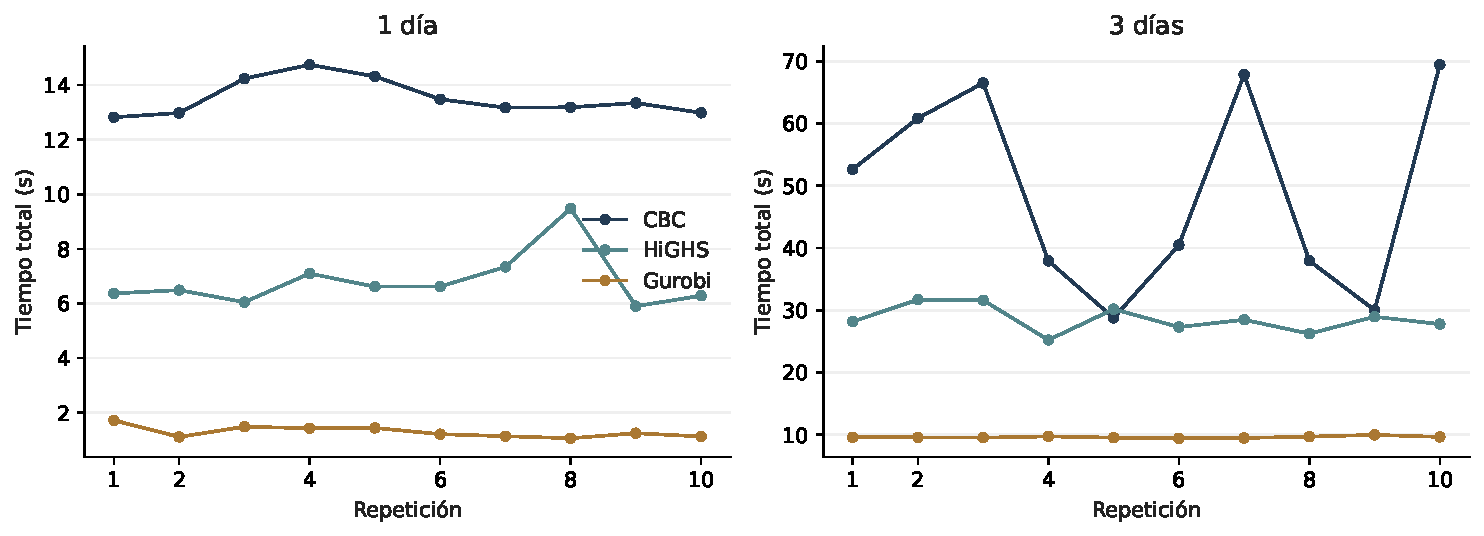
\includegraphics[width=\linewidth]{figuras/tiempos.pdf}
\caption[Tiempo por repetición y optimizador]{Tiempo total por repetición. Las escalas verticales difieren entre horizontes.}
\end{figure}

Los tiempos reportados son los totales, incluyendo todas las etapas que la aplicación mide durante cada corrida, y no sólo el tiempo de ejecución del solver central. Ambos tiempos son registrados en el anexo digital. En tres días se incluyen la compilación, la poda, los maestros y la verificación de distribución; no se puede determinar el tiempo para encontrar un inicio común a partir del tiempo medio de certificación. No hicimos experimentos de ablación para poder atribuir parte de la ganancia de tiempo a un corte o poda en particular, o a un cambio de versión o a un inicio factible.

El hecho de que los certificados sean los mismos en estas dos instancias muestra la robustez del método en estas dos instancias, pero no nos da diez demostraciones matemáticas independientes de la corrección de los datos. Se registra el identificador, la semilla, el motor, la versión, el objetivo, las cotas, la brecha, los residuos y el tiempo para poder revisarlos. Las tablas con las diez repeticiones están en el anexo~\ref{an:certificaciones}, mientras que en el texto principal sólo presentamos la síntesis del experimento nominal.

El anexo~\ref{an:desarrollo_complementario} conserva la lectura estadística de las repeticiones.

% !TeX root = ../Trabajo_RPM.tex
\section{Evaluación sobre cien instancias sintéticas}\label{sec:instancias}
En esta fase se extiende la experimentación llevada a cabo en la sección~\ref{sec:resultados} con el caso diario. Se ejecuta la regla de asignación de RPM y el MILP en cien instancias con diferentes demandas, tamaños, horizontes, capacidades y matrices de tiempos. Cada instancia es resuelta con la heurística corporativa y el solucionador CBC, HiGHS y Gurobi. Esta etapa se ilustra en la figura~\ref{fig:ruta_metodologica_rpm}, y se encuentra ubicada después de la caracterización de los datos y antes de la interpretación de planes. Mientras que los experimentos con repeticiones llevan a cabo el mismo problema, el experimento con 100 problemas consiste en observar el efecto de utilizar diferentes instancias de entrada.

\subsection{Muestra y generación de demanda}\label{sec:muestreo100}
El libro de RPM ofrece volúmenes de demanda semestrales, agrupados por referencia, pero no una serie temporal de pedidos individuales. Así, permite estudiar la heterogeneidad entre referencias, pero no permite estimar una distribución de demanda diaria para una referencia dada, ni tampoco una estacionalidad de dicha demanda. Por eso se utilizará un remuestreo estratificado transversal, y se hará explícito el supuesto necesario para utilizarlo: dentro de un volumen de demanda similar, los factores relativos de unas referencias pueden ser utilizados como donantes para construir nuevas demandas sintéticas. Esta hipótesis no es una propiedad demostrada de las ventas a través del tiempo: es el supuesto en el que se basa el experimento.

Las doscientas referencias se ordenan según sus ventas en el semestre. En caso de empate, el programa utilizado ordena por nombre, y luego divide el conjunto de referencias en tres grupos con tamaños parecidos. De esta forma se evita que la dispersión relativa de las referencias menos vendidas se mezcle directamente con la de las referencias con mayor volumen de ventas. Al mismo tiempo, se evita que alguno de los estratos quede con un número de donantes pequeño para el remuestreo con reemplazo. La tabla~\ref{tab:estratos100} muestra la dispersión de las demandas que servirá de base para el generador sintético. El coeficiente de variación del estrato de las referencias de mayor volumen de ventas es mucho mayor, y se conserva esta asimetría en el experimento en vez de aplicar a todas las referencias una perturbación aleatoria uniforme.

\begin{table}[H]\centering\small
\caption{Estratos de volumen semestral utilizados como base del remuestreo}\label{tab:estratos100}
\begin{tabular}{lrrrr}\toprule
Estrato & Referencias & Media (unidades) & Mediana & CV\\\midrule
Bajo & 67 & 3.596 & 3.439 & 0,20\\
Medio & 67 & 9.715 & 10.012 & 0,30\\
Alto & 66 & 85.758 & 32.246 & 1,60\\\bottomrule
\end{tabular}
\fuente{ventas semestrales del anexo de datos; estadísticos redondeados de \texttt{distribucion\_estratos.csv}}
\end{table}

Siendo $V_i$ la venta semestral de la referencia $i$ y $g(i)$ el estrato al que pertenece, se calcula, para cada donante $k$ del mismo grupo, el cociente $w_k=V_k/\overline V_{g(i)}$. El promedio de estos cocientes coincide con el valor 1 dentro de cada estrato. Para cada bloque $b$ se selecciona con reemplazo un donante $k(i,b)$ de ese mismo grupo que $i$ y se define la demanda del bloque $b$
\begin{equation}
	D_{ib}=\left\lfloor d_i^{\mathrm{base}}\,H_b\,\lambda_b\,\frac{V_{k(i,b)}}{\overline V_{g(i)}}+\frac12\right\rfloor,
	\label{eq:demanda100}
\end{equation}
donde $d_i^{\mathrm{base}}$ es la demanda diaria calibrada (véase el anexo \ref{an:construccion}) y $H_b$ y $\lambda_b$ son el horizonte y nivel de demanda del bloque $b$. Se ha considerado la parte entera más próxima al valor, para asegurar que la demanda sea una variable entera. Antes de aplicar esta transformación, el factor aleatorio mantiene sin alteración la demanda base en valor esperado. No ocurre lo mismo para una realización, en concreto. Los niveles de intensidad de demanda son condiciones bajo las que se experimenta, no estimas de su frecuencia en el funcionamiento real.

El diseño experimental tiene 4 niveles de intensidad de demanda (0,8; 1,0; 1,2 y 1,4), 3 tamaños de catálogo (99, 150 y 200 referencias) y 3 horizontes (1, 3 y 5 días). El número de combinaciones posibles es 36. De ellas, se ha elegido un subconjunto de 25 celdas siguiendo una regla de permutación y exclusión modular que se definió previamente al resolver los problemas. Con ella, se seleccionan 24 celdas y una adicional a éstas, elegida entre las omitidas según la semilla utilizada. Así, los niveles de demanda han sido empleados en 24, 24, 24 y 28 problemas respectivamente; los tamaños de catálogo, en 32, 32 y 36 problemas; y los horizontes, en 32, 32 y 36 problemas. Con esta fracción de diseño se incluye la experiencia de todos los niveles, pero no todos los efectos e interacciones posibles del factorial completo.

Una común modificación al catálogo del problema es hacer que existan subconjuntos anidados dentro del catálogo: los 99 productos están contenidos en los 150, los cuales están contenidos en los 200. Esto nos da una forma de manejar parcialmente como varía la composición del catálogo a medida que aumentamos su tamaño. No obstante, no consideramos todas las mezclas posibles del catálogo para igual cantidad de productos.

Cada celda de este cuadro genera un vector de demanda que se conserva en cuatro versiones: capacidad nominal o reducida en 25\,\% en M1, y matriz de demanda como fue publicada o reconstruida. La capacidad nominal es de 1.440 minutos por máquina por día, mientras que en M1 se reduce a 1.080 en la versión de capacidad reducida. Los alistamientos se mantienen en sus valores originales. De esta manera, obtenemos un total de 100 problemas distintos a partir de 25 realizaciones de demanda, sin eliminar o cambiar problemas en base a su dificultad o a si son o no factibles. La semilla utilizada para generar la demanda es 191007. En el anexo~\ref{an:instancias100} se encuentran identificadas las cien instancias y sus huellas; en el manifiesto digital se guarda la huella SHA-256 completa.

Los diferentes tamaños permiten hacer una conexión con el caso diario de 99 productos y el catálogo ampliado con 200 productos, siendo el catálogo de 150 productos un nivel intermedio. Un día permite replicar el horizonte corto, mientras que tres días permite conectarnos con el caso nominal de multiperiodo con lote, y 5 días hace que el modelo tenga que considerar un horizonte más largo. El uso de la matriz publicada y la reconstruida permite analizar la sensibilidad a los coeficientes como se hace en la sección~\ref{sec:datos}. La capacidad reducida de M1 es un ejemplo de ensayo de capacidad, y no representa una situación de parada observada en planta. Esta diferencia de datos permite no sólo analizar cómo se comparan los métodos, sino también donde una asignación conjunta supera a la regla local.

\subsection{Comparación emparejada y alcance estadístico}
La heurística implementa en forma algorítmica la regla de asignación de RPM explicada en la sección~\ref{sec:heuristica}. La extensión de esta heurística al caso multiperiodo consiste en repetir la asignación un día a la vez, ordenar la demanda insatisfecha y asignarla utilizando primero las máquinas con menor tiempo unitario disponible. La implementación de la heurística establece la forma en la que se resuelven los desempates. Todos los métodos se ejecutan sobre el mismo problema, recibiendo la misma demanda, capacidad y matriz. Como resultado, la comparación realizada no es entre diferentes heurísticas o métodos de la compañía sino que se estudia la regla utilizada por la compañía bajo diferentes entradas, controladas y conocidas. Los planes encontrados por los métodos sintéticos no deben ser tomados como los turnos que la empresa realizó en determinado momento de su historia.

Los tres motores utilizados para resolver el modelo completo del problema, presentado en la sección~\ref{sec:modelo}, tienen el mismo set de refuerzos válidos, y no se le proporciona a ninguno de los motores una solución inicial. Para verificar la correcta implementación de los motores se realizó una auditoría para chequear que el LP de cada instancia resuelto por cada motor tiene el mismo hash. Se corrió cada método una vez por cada instancia para evitar confundir la repetición de una semilla con una variedad de problemas. Se siguió un protocolo de ejecución para asignar un presupuesto de resolución a cada problema según su tamaño y horizonte. A cada problema se le asignó el mismo presupuesto de tiempo a cada uno de los motores (CBC, HiGHS, y Gurobi). Todos los motores corrieron sobre el mismo modelo con el mismo criterio de aceptación de soluciones. El detalle de este protocolo se detalla en el Anexo~\ref{an:protocolo100}. Esto significa que un problema más grande obtiene más tiempo de cómputo, en proporción a su tamaño, que uno más pequeño. Esto se hace para no favorecer a ninguno de los motores al momento de hacer la comparación. El orden de corrida de los motores se alternó entre las instancias, y debido a las diferentes condiciones de entorno donde se corrían los experimentos, las comparaciones de tiempos de resolución son más limitadas.

Si la heurística y motor resuelven el problema satisfaciendo toda la demanda, la reducción de carga es
\begin{equation}
R_{bs}=100\,\frac{Z_b^{\mathrm{heur}}-Z_{bs}}{Z_b^{\mathrm{heur}}}.
\label{eq:mejora100}
\end{equation}
Un plan parcial no es una referencia equivalente. Si en cualquiera de los dos métodos no hay demanda, el informe no hará el cálculo de la reducción, manteniendo el faltante. Tampoco el hecho que el incumbente sea mejor que la heurística lo convierte en óptimo.

Las cuatro instancias de una celda de problema tienen la demanda en común. Es decir, no son cuatro extracciones independientes. La celda comparable es la unidad sobre la que se aplica el bootstrap, manteniendo juntas las distintas variantes. Se realizaron 1.000 remuestreos con semilla 19042 en cada motor y se obtuvieron los percentiles 2,5\,\% y 97,5\,\% sobre las medias \cite{davison1997}. En el diseño hay 25 celdas, de las cuales Gurobi y HiGHS tienen 18 celdas con parejas completas, mientras que CBC tiene 16. Así, el intervalo indica el rango de variación de los resultados de las comparaciones en el diseño. El hecho que se seleccionen instancias con distintos tamaños y horizontes tampoco aísla de por sí un efecto causal, ya que las celdas tienen otras diferencias en condiciones.

\subsection{Resultados: cobertura y calidad de las soluciones}
Los cien problemas generaron los 400 registros que nos esperábamos. Las 24 instancias que los tres motores consideraron inviables fueron las mismas; a las 76 restantes se les pudo ofrecer un plan completo verificado por HiGHS y Gurobi. CBC terminó 54. La heurística consiguió encontrar una solución para 68 de las instancias y quedaron 8 de ellas con demanda insatisfecha que, sin embargo, pudo ser cubierta por el MILP. En la tabla~\ref{tab:solvers100} hemos diferenciado entre la capacidad de un plan factible y el cierre de las cotas.

\begin{table}[H]\centering\footnotesize\setlength{\tabcolsep}{5pt}
\caption{Cobertura y GAP final de la comparación central}\label{tab:solvers100}
\begin{tabular}{lrrrr}\toprule
Método & Planes completos & Óptimos acreditados & GAP mediano (\%) & GAP máximo (\%)\\\midrule
Heurística & 68 & -- & -- & --\\
CBC & 54 & 20 & 1,5423 & 13,3623\\
HiGHS & 76 & 31 & 0,6324 & 3,6061\\
Gurobi & 76 & 41 & 0,0100 & 0,1795\\\bottomrule
\end{tabular}
\fuente{consolidado de 400 registros. El GAP mediano y el GAP máximo se afectan únicamente por los planes completos sin certificado: 34 de CBC, 45 de HiGHS y 35 de Gurobi. Las 24 inviabilidades concordantes no conforman esas medianas}
\end{table}

Con Gurobi, los 76 planes completos alcanzan un GAP menor que 0,18\,\%; 68 planes tienen un GAP no mayor a 0,1\,\%. Lo cual implica que la brecha relativa entre el valor objetivo obtenido y una cota inferior válida es pequeña. El resultado de los 5 días se mantiene similar: en dicho periodo se tienen 32 planes completos, de los cuales nueve tienen un óptimo acreditado, y un GAP máximo de 0,179452\,\%. Para el caso de E097 con 200 referencias y 5 días se tiene que $LB=49.591,9587946$ y $UB=49.591,9587963$ minutos, lo cual representa un GAP de apenas $3,43\times10^{-9}\,\%$. Con el criterio de verificación, se acreditan 41 óptimos, y los otros 35 planes completos tienen cotas cercanas, representando asignaciones factibles.

\subsection{Comparación con la regla de RPM y perfil de factores}
En la tabla \ref{tab:mejora100} únicamente aplicamos la ecuación~\eqref{eq:mejora100} si ambos planes sirven a un mismo pedido. Para las 68 parejas de soluciones completas proporcionadas por Gurobi, el MILP proporciona una mejora media del 21,8\,\% sobre la carga nominal, con un intervalo de confianza bootstrap del 19,5\,\% al 24,8\,\%. Todas las 68 mejoras son positivas. Para el subconjunto de problemas para los que los tres motores fueron capaces de encontrar soluciones (48 problemas), las medias de mejora son del 21,4\,\% para CBC, del 23,1\,\% para HiGHS y del 23,2\,\% para Gurobi. Esta comparación mantiene fijo el conjunto de problemas.

\begin{table}[H]\centering\small
\caption{Reducción de carga frente a la heurística de RPM en parejas completas}\label{tab:mejora100}
\begin{tabular}{lrrrr}\toprule
Motor & Parejas & Media (\%) & Mediana (\%) & IC 95\,\% (\%) \\
\midrule
CBC & 48 & 21,4 & 20,6 & [17,9; 24,9] \\
HiGHS & 68 & 21,4 & 20,2 & [18,9; 24,5] \\
Gurobi & 68 & 21,8 & 20,3 & [19,5; 24,8] \\
\bottomrule\end{tabular}

\fuente{\texttt{comparacion\_heuristica\_100.csv}. El intervalo remuestrea las celdas comparables, no cada variante por separado; el número de parejas difiere entre motores}
\end{table}

La figura~\ref{fig:perfil100} recupera la comparación por factores de tiempo: para cada instancia con algún óptimo acreditado, divide el tiempo de cierre de cada motor por el menor tiempo acreditado de esa misma instancia \cite{dolan2002}. El factor 1 identifica al primero; un método sin cierre conserva factor infinito. El perfil mantiene como denominador los 76 problemas con plan completo. Gurobi alcanzó el primer cierre en 41 de las 42 instancias donde algún motor acreditó el óptimo; HiGHS lo hizo en la restante. Los tiempos también dependen del hardware de los trabajadores remotos. El perfil caracteriza este protocolo de ejecución y no constituye una clasificación universal de velocidad.

\begin{figure}[H]\centering
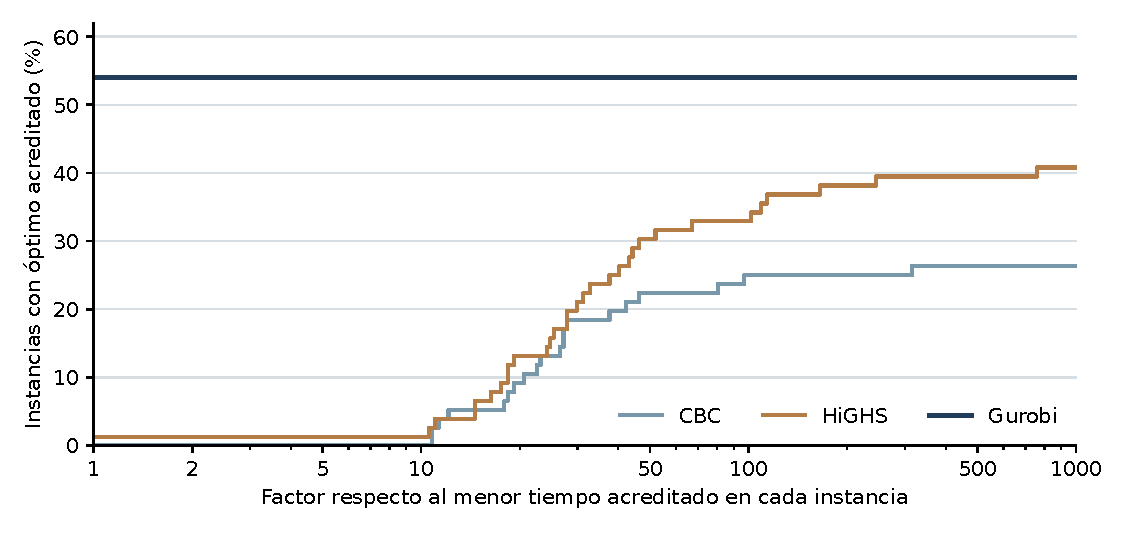
\includegraphics[width=.90\linewidth]{figuras/perfil_factores_100.pdf}
\caption{Proporción de las 76 instancias con solución factible para las que cada motor acredita el óptimo dentro del factor de tiempo indicado. Los casos sin certificado no alcanzan un factor finito.}\label{fig:perfil100}
\fuente{\texttt{consolidado\_400.csv}; cálculo reproducible en \texttt{generar\_resultados\_estratificados.py}}
\end{figure}

En la instancia nominal diaria, el modelo MILP reduce la carga agregada de producción un 15,6\,\% frente a la heurística de referencia. Por su parte, el Monte Carlo histórico tiene un valor promedio cerca del 15,2\,\% bajo la misma perturbación de demanda. Para este estudio se usaron 100 problemas en los que se modifica el tamaño, el horizonte, la matriz y la capacidad. Estas corridas no se agregan a la media. La ventaja en carga obtenida es para planes similares bajo los supuestos del modelo. En el anexo~\ref{an:instancias100} es posible localizar el estado y el GAP de cada instancia.


\section{Sensibilidad y Monte Carlo histórico}\label{sec:escenarios}
El escenario estudia el efecto sobre los resultados cuando cambian los datos. Utiliza la toma de decisiones previamente desarrollada, pero hace un tipo de análisis diferente al de la certificación nominal. En la sensibilidad actual de demanda y capacidad se usa el protocolo que no tiene el límite interno. El Monte Carlo mantiene la distribución, los criterios de terminación, y los archivos de historias. Estos resultados son de un experimento distinto al de las 60 corridas nominales.

\subsection{Dependencia respecto de los coeficientes}
Una vez realizada la revalidación histórica con la matriz reconstruida, el óptimo diario fue de 11.430 minutos, frente a los 11.547 minutos de la matriz nominal. Se registraron 21 cambios de asignación. Este resultado no puede ser entendido como una mejora del algoritmo, a nivel operativo, debido a que los coeficientes del problema no son los mismos. Si evaluamos el plan nominal sin reoptimizar con la matriz reconstruida obtenemos un resultado de 11.973 minutos. Comparando los dos resultados podemos observar como la procedencia de los tiempos en la toma de decisiones, puede ser más importante que las pequeñas diferencias entre las configuraciones del solver.

La ejecución actual de sensibilidad de capacidad identifica a M8 como el recurso con mayor respuesta al incremento evaluado: 30 minutos adicionales reducen el objetivo en 5,4161 minutos. M7 y M9 aportan reducciones de 3,2289 y 0,3550 minutos; las otras siete máquinas registran cero a la precisión mostrada. El cociente $\eta_j=[Z(K)-Z(K+30e_j)]/30$ mide una diferencia finita, no un precio sombra del MILP. La tabla~\ref{tab:capacidad_actual} recoge los resultados que muestra la aplicación.

En sensibilidad de demanda, la aplicación resuelve cinco factores entre 0,8 y 1,2 después de convertir la demanda escalada en unidades enteras. Los cinco escenarios muestran estado óptimo y GAP reportado cero. Para el factor 1,2, el objetivo es de 13.641,1764 minutos; el caso base conserva 11.547 minutos. La tabla~\ref{tab:sensibilidad_actual} identifica la demanda efectiva y los objetivos de esta ejecución.

\subsection{Escenarios de demanda}
Con un ejercicio histórico de Monte Carlo se han generado 1.000 demandas y reoptimizado cada escenario a partir de factores uniformes e independientes que van de 0,85 a 1,15. Hay que tener en cuenta que la distribución es una hipótesis de tipo experimental y no una estimación validada de los pedidos reales. Reoptimizar tras ver una demanda no acredita que el plan nominal siga siendo viable ante dicha perturbación.

Según lo expuesto en el documento de base, la revalidación deja constancia de 1.000 comparaciones factibles entre MILP y heurística. No hay GAP numéricamente cero en ninguna; el máximo se sitúa en 1,1879\%. En cuanto a los incumbentes, la mejora media ha sido del 15,2\% (15,2\% de mediana) y con una desviación estándar de 0,7724 puntos porcentuales. Las cotas ubican la media óptima de la muestra en un tramo entre 15,2\% y 15,3\%, un rango que describe la incertidumbre de optimización más que de un intervalo de confianza de la población.

Estos valores son de carácter histórico y se cotejan con los CSV obtenidos, sin que se trate de una nueva simulación para esta revisión. El anexo~\ref{an:historico} guarda el procedimiento y hace la salvedad de las cifras de 15,14\% de una ejecución anterior. Tampoco las 60 certificaciones nominales vienen a sustituir los registros de los 1.000 escenarios o a hacer óptimos sus incumbentes.

El anexo~\ref{an:desarrollo_complementario} presenta el generador y las verificaciones de Monte Carlo.

\section{Aplicación, evidencia y uso operativo}\label{sec:aplicacion}
Esta aplicación hace un recuento de las salidas del recorrido metodológico, es decir, los datos identificados, los planes, los indicadores y la evidencia de resolución. La certificación respalda las instancias nominales y son los escenarios los que se encargan de su interpretación. El usuario tiene a mano ambas fuentes con el estado de cada una para descargar los archivos y pasar revista a las decisiones tomadas.

Por su parte, la herramienta computacional articula la carga de datos, la opción de horizonte y la resolución para proceder a la descarga de resultados. En este caso lo valioso es que mantiene un vínculo comprobable entre lo que se ha introducido y lo que se obtiene. Un plan descargado ha de dejar constancia de la instancia, los parámetros y el estado de solución de origen; con una hoja que diga ``óptimo’’ pero carente de cotas o validación no se tiene suficiente prueba.

Los resultados se exponen técnicamente diferenciando el valor objetivo y sus partes, la demanda de referencia, la carga, holgura y uso por máquina y día, las preparaciones, el estado de terminación, $LB$, $UB$ y GAP, la duración, qué versión de motor se emplea y los residuos de verificación. Con la demanda invariable, la interfaz se encarga de calcular el horizonte mínimo. El indicador da a ver tres días para el lote nominal y en la comparación se tienen en cuenta los supuestos de uno y tres días. Los módulos de certificación de costes y de verificación de días mínimos se han implementado como módulos separados. Un plazo sin resolver no es una situación óptima.

Para el plan y el informe, la aplicación permite la descarga en tres niveles: plan diario, plan de multiperiodo y archivo de certificación. Aunque el plan incluye solo la activación y el número de unidades, el archivo de certificación incluye estos datos más parámetros, logs y matrices. El inventario de pruebas para los archivos de certificación se pueden ver en el anexo~\ref{an:repro}. En los archivos de certificación no se incluye la información de licencia, que no es necesaria para la certificación del motor que se utiliza.

La herramienta podría ser implementada por RPM de manera gradual. El equipo en planta debería comprobar la compatibilidad de los pares de equipo que están actualmente activos, los tiempos en los que se concentra la carga, y la capacidad neta que se debería utilizar (en lugar de la capacidad nominal). Una vez esto se haya comprobado, se puede llevar a cabo un piloto con el plan, y guardar información de las preparaciones, las incidencias y la producción. Esta información permitiría cuantificar el impacto del plan en la operación, aparte de la mejora que se obtenga del uso del motor.

En el anexo~\ref{an:desarrollo_complementario} se describe cómo se han implementado los controles de carga y exportación de la aplicación.


\section{Discusión de los hallazgos y alcance operativo}
La limitación más importante de nuestro estudio es que solo se cuenta con trazabilidad parcial de los tiempos. Aunque podemos controlar una regla de imputación para las celdas observadas, esto no nos permite hablar abiertamente del proceso generador de los tiempos que componen la matriz nominal publicada. El hecho de que nuestro modelo de programación resuelva satisfactoriamente la matriz nominal mencionada no implica que no sea conveniente contar con una regla de imputación que pueda ser validada técnicamente; el documento indica esta dualidad.
Nuestro modelo asume que las máquinas tienen una capacidad nominal de 24 horas por día y no hace ningún tipo de ajuste por fallos, mantenimientos o uso en común de las máquinas. Suponemos que los alistamientos no dependen de la secuencia ni del producto. En caso de que fuese necesario, por ejemplo, mantener un alistamiento entre días o que éste dependa del producto, habría que incluir variables y parámetros adicionales en el modelo, lo que cambiaría su formulación y nos obligaría a recalcular los planes y sus certificados.

El modelo asume que la demanda está disponible desde el comienzo y se debe satisfacer en una ventana común. La función objetivo no considera clientes y no penaliza la tardanza. Tampoco contempla la reposición de inventarios con realimentación. Así, nuestro modelo se limita a un problema de asignación estática de producción. La incertidumbre operativa, la secuencia y la planificación dinámica necesitarían datos y formulaciones adicionales. La comparación central del estudio se realiza con 100 instancias y una única ejecución de cada uno de los métodos, sin considerar un inicio heredado. Tanto HiGHS como Gurobi resuelven 76 problemas del total que resultan ser factibles, aunque Gurobi logra certificar más óptimos y presenta la menor brecha máxima con el protocolo de comparación seguido. Las dos instancias nominales mantienen el inicio informado y la estrategia selectiva y se presentan como casos ilustrativos. El remuestreo transversal nos permite incrementar la diversidad de problemas, pero no sustituye a una serie temporal de pedidos. La estratificación y la selección previa de celdas que llevamos a cabo acotan los intervalos y contrastes del estudio.

La verificación independiente re-calcula la demanda, capacidad, enlace, integralidad, no-negatividad y objetivo para los planes que hemos exportado. Para el horizonte de tres días, reconstruye la activación para los bloques que están produciendo. Los logs atestiguan las cotas y terminación. Como esta verificación se limita a los 1,000 planes históricos que ya tenemos, y los nominales, no es una sustitución por una auditoría formal de los optimizadores, ni atestigua sobre los cronometrajes del optimizador. No requiere poner de nuevo en marcha los optimizadores.

\section{Conclusiones}
Los experimentos a 100 instancias avalan la propuesta de realizar la asignación de referencias en parejas para máquinas dentro de los supuestos del modelo. La heurística logró resolver 68 instancias, y Gurobi pudo encontrar una solución completa para 76 de ellas. Los 8 casos restantes corresponden a situaciones donde la regla de asignación de referencias deja demanda insatisfecha. Gurobi consiguió para las instancias que resolvió completamente una reducción promedio en la carga de un 21,8\,\%. El intervalo de confianza del 95\,\% del bootstrap condicional, de 19,5\,\% a 24,8\,\%, debe interpretarse como la incertidumbre que hay en el diseño del sistema de referencia y en las instancias de Gurobi a las que se pueden comparar; no es un intervalo para pronosticar el ahorro que se tendrá en instancias futuras.

A partir de la caracterización, se ha podido determinar el nivel de cobertura de esta y el origen de los tiempos utilizados en el caso RPM Colombia. Gracias a los 819 pares de los 990 que tiene el caso diario, ha sido posible diferenciar entre los coeficientes e información que fueron medidos y los que no lo fueron. Al contrastar el resultado con la matriz reconstruida y el plan de fabricación obtenido se pueden saber cuales de estos datos deben ser verificados en planta. Aunque las agrupaciones permiten caracterizar la heterogeneidad de referencias, no determinan el horizonte de producción.

El MILP determina simultáneamente tamaños de lote enteros, encendidos y capacidad utilizada. Con el plan diario, se han satisfecho 14.188 unidades con una utilización de 11.547 minutos (un 15,6\,\% menor que el plan factible). La capacidad agregada del plan se sitúa en el 80,2\,\%, aunque hay máquinas cuya carga es muy alta y otras con mayor holgura. Si se realiza un análisis por recursos se puede observar este tipo de diferencias que no son visibles a nivel global.

Para el lote de 200 referencias con 45.987 unidades en total, se obtiene un valor óptimo certificado de 34.132 minutos. Al obtener una cota inferior para la carga total, se eliminan dos de los días y el plan factible asume que se necesita al menos tres días. El lote utilizado se ha creado a partir del ajuste de ventas y de la capacidad documentada, y no es un lote real de tres días concretos que se va a describir en la conclusión.

Para el problema principal de estudio, CBC ha logrado certificar el óptimo numérico en 20 casos, HiGHS en 31, y Gurobi en 41. Todos los solvers dan las mismas 24 instancias como infactibles. Gurobi ha resuelto las otras 76 instancias, obteniendo siempre un valor del GAP por debajo del 0,18\,\% en cada plan. El máximo de los GAP de las 32 instancias factibles con cinco días fue de 0,179452\,\%. Al analizar los resultados por factores, se observa que Gurobi logra el primer óptimo certificado en 41 de las 42 instancias en las que algún solver ha logrado certificar el óptimo numérico, al menos para la ejecución realizada.

Monte Carlo mantiene 1.000 casos perturbados como prueba histórica adicional. En todos los escenarios los incumbentes que resultan factibles superan a la heurística y alcanzan una reducción promedio de 15,2\%, pero no pueden ser calificados con el nombre, pues las brechas son positivas. Lo que se ve aquí es que con reoptimización bajo los supuestos de simulación el plan se adapta, pero no es una prueba de que un plan fijo sea robusto.

La aplicación une los datos, los planes, los indicadores y la evidencia que se puede exportar para apoyar la asignación. Para utilizarlo operacionalmente hay que verificar compatibilidades, medir tiempos de interés y verificar capacidades nominales contra efectivas. Esta investigación demuestra la mejora en carga computacional, y corresponderá a un piloto en planta determinar el impacto operacional y si se traduce a una mejora económica o de servicio.

La generación estratificada aprovecha la diferencia entre referencias tal como se observa, sin inventar fechas de venta. El supuesto de intercambiabilidad y la proporción de celdas seleccionadas son parte del supuesto sobre el cual se interpreta. El siguiente paso para RPM es comenzar a registrar pedidos fechados y capacidad neta, y así validar el modelo operacionalmente. Los resultados obtenidos muestran que sí hay una evaluación piloto por hacerse con respecto a la asignación, pero no una declaración de que la mejora económica ya ha sido lograda.

\clearpage
\phantomsection\addcontentsline{toc}{section}{Referencias}
\begin{thebibliography}{99}\small
\bibitem{taha} Taha, H. A. (2017). \textit{Operations Research: An Introduction}, 10.ª ed. Pearson.
\bibitem{cattrysse} Cattrysse, D. G. y Van Wassenhove, L. N. (1992). A survey of algorithms for the generalized assignment problem. \textit{European Journal of Operational Research}, 60(3), 260--272. \url{https://doi.org/10.1016/0377-2217(92)90077-M}.
\bibitem{unlu} Unlu, Y. y Mason, S. J. (2010). Evaluation of mixed integer programming formulations for non-preemptive parallel machine scheduling problems. \textit{Computers \& Industrial Engineering}, 58(4), 785--800. \url{https://doi.org/10.1016/j.cie.2010.02.012}.
\bibitem{law} Law, A. M. (2015). \textit{Simulation Modeling and Analysis}, 5.ª ed. McGraw-Hill.
\bibitem{rousseeuw} Rousseeuw, P. J. (1987). Silhouettes: A graphical aid to the interpretation and validation of cluster analysis. \textit{Journal of Computational and Applied Mathematics}, 20, 53--65. \url{https://doi.org/10.1016/0377-0427(87)90125-7}.
\bibitem{ward} Ward, J. H. (1963). Hierarchical grouping to optimize an objective function. \textit{Journal of the American Statistical Association}, 58(301), 236--244. \url{https://doi.org/10.1080/01621459.1963.10500845}.
\bibitem{cbc} COIN-OR. \textit{CBC User's Guide: Introduction}. Documentación oficial. \url{https://coin-or.github.io/Cbc/intro.html}. Consulta: 19 de octubre de 2026.
\bibitem{highs} HiGHS. \textit{List of options}. Documentación oficial, parámetros \texttt{mip\_rel\_gap} y \texttt{mip\_abs\_gap}. \url{https://ergo-code.github.io/HiGHS/dev/options/definitions/}. Consulta: 19 de octubre de 2026.
\bibitem{gurobi} Gurobi Optimization. \textit{Optimizer Reference Manual: Parameter Reference}. Parámetros MIPGap y MIPGapAbs. \url{https://docs.gurobi.com/projects/optimizer/en/current/reference/parameters.html}. Consulta: 19 de octubre de 2026.

\bibitem{mula} Mula, J., Poler, R., García-Sabater, J. P. y Lario, F. C. (2006). Models for production planning under uncertainty: A review. \textit{International Journal of Production Economics}, 103(1), 271--285. \url{https://doi.org/10.1016/j.ijpe.2005.09.001}.
\bibitem{dauzere} Dauzère-Pérès, S., Ding, J., Shen, L. y Tamssaouet, K. (2024). The flexible job shop scheduling problem: A review. \textit{European Journal of Operational Research}, 314(2), 409--432. \url{https://doi.org/10.1016/j.ejor.2023.05.017}.
\bibitem{li} Li, Z. e Ierapetritou, M. (2008). Process scheduling under uncertainty: Review and challenges. \textit{Computers \& Chemical Engineering}, 32(4--5), 715--727. \url{https://doi.org/10.1016/j.compchemeng.2007.03.001}.
\bibitem{fisher} Fisher, M. L. (1981). The Lagrangian relaxation method for solving integer programming problems. \textit{Management Science}, 27(1), 1--18. \url{https://doi.org/10.1287/mnsc.27.1.1}.
\bibitem{miplib} Gleixner, A. et al. (2021). MIPLIB 2017: data-driven compilation of the 6th mixed-integer programming library. \textit{Mathematical Programming Computation}, 13, 443--490. \url{https://doi.org/10.1007/s12532-020-00194-3}.
\bibitem{pedregosa} Pedregosa, F. et al. (2011). Scikit-learn: Machine learning in Python. \textit{Journal of Machine Learning Research}, 12(85), 2825--2830. \url{https://jmlr.org/papers/v12/pedregosa11a.html}.
\bibitem{bertsimas} Bertsimas, D. y Sim, M. (2004). The price of robustness. \textit{Operations Research}, 52(1), 35--53. \url{https://doi.org/10.1287/opre.1030.0065}.
\bibitem{pulpstart} COIN-OR. \textit{PuLP: How to warm-start a solver}. Documentación oficial. \url{https://coin-or.github.io/pulp/guides/how_to_mip_start.html}. Consulta: 19 de octubre de 2026.
\bibitem{numeric} Gurobi Optimization. \textit{Tolerances and user-scaling}. Documentación oficial. \url{https://docs.gurobi.com/projects/optimizer/en/current/concepts/numericguide/tolerances_scaling.html}. Consulta: 19 de octubre de 2026.
\bibitem{streamlit} Streamlit. \textit{Add statefulness to apps: Session State}. Documentación oficial. \url{https://docs.streamlit.io/develop/concepts/architecture/session-state}. Consulta: 19 de octubre de 2026.
\bibitem{dolan2002} Dolan, E. D. y Moré, J. J. (2002). Benchmarking optimization software with performance profiles. \textit{Mathematical Programming}, 91, 201--213. \url{https://doi.org/10.1007/s101070100263}.
\bibitem{davison1997} Davison, A. C. y Hinkley, D. V. (1997). \textit{Bootstrap Methods and their Application}. Cambridge University Press. \url{https://doi.org/10.1017/CBO9780511802843}.
\end{thebibliography}
\label{finprincipal}
\clearpage
\appendix
\setstretch{1.08}\small
\renewcommand{\thepage}{A-\arabic{page}}\setcounter{page}{1}
\fancyhead[R]{\small Anexos técnicos}
\section*{Anexos técnicos y evidencia de respaldo}
Con estos anexos se da apoyo al trabajo. Los anexos utilizan numeración de páginas con el prefijo A-. Las tablas de certificación se extienden a diez repeticiones por motor y horizonte. En el caso de la evidencia digital, los registros nativos y su exactitud se conservan; las cifras impresas, en cambio, han sido redondeadas para que resulten más legibles.

\begin{itemize}
	\item Anexo A: trazabilidad de los datos y reconstrucción histórica.
	\item Anexo B: validez de cotas y certificación selectiva.
	\item Anexo C: protocolo y sesenta certificaciones.
	\item Anexo D: sensibilidad de los resultados en vigor y antecedentes de simulación.
	\item Anexo E: verificación independiente y reproducción documental.
	\item Anexo F: heurística e instancias construidas.
	\item Anexo G: maestro, distribución diaria y poda lagrangiana.
	\item Anexo H: resultados individuales de las cien instancias y trazabilidad de la ejecución.
	\item Anexo I: desarrollo técnico complementario de métodos, datos y aplicación.
\end{itemize}

\section{Trazabilidad de los datos}\label{an:datos}
\subsection{Cobertura observada de la instancia diaria}
La documentación de origen registra hasta 30 mediciones por combinación procesada. La cobertura por máquina es la siguiente. Estos conteos pertenecen al análisis histórico del documento de base, no se infieren de la matriz C completada de los certificados.
\begin{table}[H]\centering
\caption{Pares con observación por máquina, de 99 posibles}
\begin{tabular}{lrrrrrrrrrr}\toprule
Máquina&M1&M2&M3&M4&M5&M6&M7&M8&M9&M10\\\midrule
Observados&35&67&89&74&83&93&97&95&95&91\\\bottomrule
\end{tabular}
\end{table}
La suma es 819; los 171 faltantes representan el 17,27\%. Una celda sin medición se debe identificar mediante una marca de procedencia, sin confundir el valor estimado con un cronometraje. La evaluación de compatibilidad técnica debe ser independiente de la presencia de observación.

\subsection{Comparación de estimadores}
Con un conjunto de prueba $V$ de celdas observadas ocultadas, se utilizan
\begin{align}
\mathrm{MAE}&=\frac{1}{|V|}\sum_{(i,j)\in V}|C_{ij}-\widehat C_{ij}|,\\
\mathrm{RMSE}&=\sqrt{\frac{1}{|V|}\sum_{(i,j)\in V}(C_{ij}-\widehat C_{ij})^2}.
\end{align}
Los parámetros de cada estimador deben calcularse sin usar las celdas ocultadas. La media por máquina se estima con observaciones positivas del conjunto de entrenamiento de cada equipo. La exclusión de ceros requiere distinguir ausencia de dato de un valor físico válido; un procesamiento de duración cero no se interpreta como alternativa gratuita.
\begin{table}[H]\centering\small
\caption{Revalidación histórica de imputación, 100 particiones}
\begin{tabular}{lrrr}\toprule
Estimador&MAE medio&IC reportado del 95\%&Mejor en\\\midrule
Media por máquina&0,1888&[0,1869; 0,1906]&96/100\\
Media global&0,1992&[0,1975; 0,2010]&3/100\\
Modelo aditivo&0,2066&[0,2046; 0,2086]&1/100\\
Media por referencia&0,2180&[0,2159; 0,2201]&0/100\\\bottomrule
\end{tabular}
\fuente{revalidación documento de base; MAE en min/unidad}
\end{table}
Las particiones reutilizan una base de observaciones. El intervalo reportado resume la variación del error en esa evaluación; no estima la incertidumbre de todas las celdas sin observación ni demuestra un muestreo aleatorio de la producción de la empresa.

\subsection{Diferencias entre matriz publicada y reconstruida}
El documento de base reporta concordancia entre los coeficientes publicados en \texttt{MODELO PL} y \texttt{DATOS SIMULADOS}, tras convertir segundos a minutos y aplicar una tolerancia de $10^{-6}$. La reconstrucción con las medias positivas por máquina difiere de la matriz publicada en 174 celdas: 171 pares sin observación y tres con registro. Ninguna de las 171 imputaciones publicadas coincide con la media por máquina reconstruida dentro de esa tolerancia. La comparación identifica una discrepancia de procedencia; no autoriza a sustituir los coeficientes conservando los certificados originales.

\begin{table}[H]\centering\small
\caption{Discrepancias históricas en tres pares con observación}
\begin{tabular}{p{73mm}rr}\toprule
Par & Publicado & Reconstruido\\\midrule
M1: SOBRETAPA VV VERDE SF QUALA &0,392222&0,405747\\
M1: ENVASE 4 LTS SUAVIZANTE AZUL PE &0,075000&0,450000\\
M5: MAQUILA ENV 400 CRISTAL 17 GR S.M. PET CAPRI &1,147407&0,562222\\\bottomrule
\end{tabular}
\fuente{revisión histórica de cronometrajes; unidades min/unidad}
\end{table}
En el primer par se constata un cero en 30 registros, a diferencia del segundo que cuenta con cinco observaciones positivas de ese mismo total. En lo que atañe al tercer par, la divergencia entre las hojas no se debe a una simple conversión de unidades. La matriz de publicación se queda con el resultado nominal y la reconstrucción pasa a ser un análisis de alternativa. Hacer otra cosa y cambiar los coeficientes sin más sería imposible para conciliar planes y certificados.

\subsection{Agrupaciones y límites de interpretación}
$D_i$ y $CV_i=\sigma(C_{i\cdot})/\mu(C_{i\cdot})$ son los parámetros que se usan para la segmentación histórica de los productos. Un valor de $CV_i$ bajo indica una relativa similitud en los tiempos nominales, aunque no debe tomarse como indicio de que existan moldes disponibles o capacidad remanente, ni de compatibilidad. En cuanto a los grupos 42, 52 y 5, su carácter es descriptivo; con dos bastaría para maximizar Silhouette en el análisis, pero se ha optado por tres en aras de la interpretación.

Para el agrupamiento de las máquinas se ha tenido en cuenta el tiempo de alistamiento y la media y varianza de operación. M1 y M10 se erigen en grupos separados y el resto de los ocho equipos forman un tercer grupo. La concordancia con Ward da un índice de Rand ajustado de 1,000. Conviene precisar que esto indica una coincidencia entre las dos particiones y no que todas las máquinas sean del mismo grupo, pues el índice es de particiones y no de homogeneidad general.

Las pruebas de Kruskal--Wallis sobre las variables de las agrupaciones no se toman como validación inferencial independiente. De igual modo, un alto alistamiento no se considera algo “mejor”; M2 tiene uno de los tiempos más elevados, lo que en el modelo implica una carga de preparación mayor.

\section{Cotas y fundamento de la certificación selectiva}\label{an:prueba}
\subsection{Validez de la cota de enlace}
Si $x_{ijt}>0$, el enlace exige $y_{ijt}=1$. La capacidad local implica $C_{ij}x_{ijt}+S_j\leq K_{jt}$ al omitir términos no negativos de otras referencias. Como $C_{ij}>0$ y $x_{ijt}$ es entero,
\[
x_{ijt}\leq\left\lfloor\frac{K_{jt}-S_j}{C_{ij}}\right\rfloor.
\]
De la igualdad de demanda y la no negatividad se deduce que $x_{ijt}\leq D_i$. Es válida la menor de las dos cotas. En el caso de que el presupuesto no dé para una unidad y su preparación, el par ha de fijarse sin producción. La cota se vuelve a calcular ante cualquier variación en la demanda, los tiempos o la capacidad.

\subsection{Cota de horizonte}
En un plan de viabilidad, toda unidad de $i$ hace un consumo de por lo menos $\min_j C_{ij}$ y cada referencia positiva activa una preparación cuya duración no es inferior a $\min_jS_j$. La suma de los dos da la ecuación~\eqref{eq:cotaH}. Dado que la carga de un plan no puede exceder la capacidad del horizonte en su totalidad, si $L(D)>\sum_{j,t}K_{jt}$ el plan es infactible. La demostración utiliza cantidades no negativas y al menos una activación para cada referencia con demanda positiva; no comparte un único alistamiento entre referencias distintas.

Con el lote fijo certificado se tiene un $L(D)$ de 29.748,49444444444 minutos. Puesto que la capacidad para dos días es de 28.800, el margen de 948,4944 minutos basta para descartar dicho horizonte, aún con elecciones de máquina lo más optimistas que sean. La cota descarta dos días y el plan factible de tres demuestra el horizonte mínimo, sin necesidad de resolver la instancia incompatible de dos días.

\subsection{Maestro relajado y plan completo}
Dado que $\mathcal F$ es el conjunto factible del modelo en su forma totalmente desagregada y $\mathcal R$ un maestro que hace una relajación de algunas de las restricciones diarias, si todo plan de $\mathcal F$ se puede representar en $\mathcal R$ sin un objetivo mayor, el óptimo del maestro constituye una cota inferior. Con un plan completo $\bar x\in\mathcal F$ a mano,
\[
Z_{\mathcal R}^*\leq Z_{\mathcal F}^*\leq Z(\bar x).
\]
El óptimo del modelo entero queda certificado cuando los extremos concuerdan según el criterio numérico en vigor. No es suficiente con la factibilidad de una distribución parcial; el plan de cierre ha de satisfacer tanto la demanda como la capacidad máquina por día.

De las corridas de tres días se han documentado dos maestros. El primero, en su forma agregada, da 34.131,057833 minutos, pero al comprobar la distribución para M1 resulta infactible. El maestro de después incluye M1 por día y llega a 34.132,1433888890 minutos. El plan completo validado alcanza 34.132,1433888889. Las diferencias entre cotas son del orden de $10^{-10}$ minutos, muy inferiores a $10^{-5}$; el anexo~\ref{an:repro} presenta el máximo observado sobre las 60 corridas.

Que un subproblema de distribución sea infactible no implica lo mismo para el problema de producción en su totalidad. Lo que indica es que la asignación agregada no se puede repartir con las decisiones ya tomadas en ese subproblema. Habrá que añadir detalle o rectificar la asignación, como se ha hecho en este caso.

\subsection{Poda y preservación del óptimo}
En el espacio de decisiones, una cota $L_B$ válida para una región condicional $B$ posibilita su descarte cuando $L_B>UB+\varepsilon$, con $\varepsilon$ como margen conservador. Debe tenerse en cuenta que si se aplica el criterio de no mejora hay que mantener por lo menos la solución factible de la que se deriva $UB$. Una evaluación heurística sin cota válida no justifica descartar regiones.

Los datos de la corrida CBC 1 de tres días documentan una cota lagrangiana de 34.070,609557 minutos y un comienzo de 34.132,143389, con un margen de 0,0003639826 y 579 pares puestos a cero. Dicha cota lagrangiana es de entrada, no la cota final de certificación. El cierre definitivo se obtiene del maestro resuelto y del plan verificado en su totalidad. La auditoría documental comprueba los registros y sus huellas, pero no certifica haber revisado formalmente cada operación de programación dinámica del código de origen.

\subsection{Simetría y ausencia de límites internos}
La variedad de tiempos y preparaciones no permite considerar a las diez máquinas como meras copias intercambiables. Si en un día se dan iguales capacidades y no hay fechas internas, es posible que se presenten permutaciones en las etiquetas de día sin perder el objetivo ni la factibilidad; una ruptura de la simetría ha de tener su justificación en tal estructura. Un grupo descriptivo de las máquinas no da pie a establecer un orden de carga entre unas y otras. Pedir brechas cero no quiere decir que de por sí todas las instancias venideras vayan a concluir con celeridad. El criterio numérico de la corrida y el límite de recursos del entorno son condiciones diferentes. Una interrupción externa se debe reportar como tal, conservando incumbente y cota si existen, sin renombrar el estado como óptimo.

\clearpage
\section{Protocolo y tablas de certificación}\label{an:certificaciones}
\subsection{Configuración conservada}
\begin{table}[H]\centering\small
\caption{Configuración del experimento de certificación}
\begin{tabular}{p{49mm}p{100mm}}\toprule
Elemento & Valor registrado\\\midrule
Fecha de ejecución & 25 de octubre de 2026, Colombia; 26 de octubre, UTC\\
Instancias & 99 referencias/1 día; 200 referencias/3 días\\
Repeticiones & 10 por motor e instancia; 60 en total\\
Semillas & 42, 43, \ldots, 51\\
Hilos solicitados & 1 por solver; 16 CPU lógicas disponibles\\
Límite interno de tiempo & Ninguno; valor nulo en el protocolo\\
Brechas solicitadas & Relativa = 0; absoluta = 0\\
Tolerancia de verificación & $10^{-5}$, con residuos y unidades identificados\\
Cierre de cotas & Diferencia absoluta $\leq10^{-7}$ min y brecha relativa $\leq10^{-9}$; estado óptimo y plan válido\\
Inicio diario & Heurística determinista factible\\
Inicio de tres días & Plan común obtenido previamente con HiGHS\\
Orden & Horizonte diario completo, luego tres días; motores alternados\\
Sistema & Linux 6.12.94+, x86\_64; modelo físico de CPU no registrado\\
Python / PuLP & 3.14.9 / 3.3.0\\
Versiones de motores & CBC Devel/cbcbox 2.924; HiGHS 1.15.1; Gurobi 13.0.3\\\bottomrule
\end{tabular}
\end{table}

CBC registra preprocesamiento, cortes Gomory, mochila y probing, heurísticas activas, ramificación fuerte con valor 5, incremento de objetivo cero y las dos semillas. Su línea de ejecución contiene \texttt{-ratio 0.0}, \texttt{-allow 0.0} y \texttt{-threads 1}; no contiene una orden de corte por segundos. La opción \texttt{timeMode elapsed} indica cómo se contabiliza el tiempo, no establece un límite. La versión usada se identifica por la huella del ejecutable en el protocolo.

Las tablas siguientes presentan cotas con seis decimales y duración con tres. En cada una de las 60 filas, el estado es óptimo certificado numéricamente y la verificación del plan cumple. El CSV digital conserva cifras sin este redondeo, brecha absoluta, tiempos de solver, preparación, producción y huellas.

\clearpage
\subsection{Diez repeticiones por motor: un día}
{\small\setlength{\tabcolsep}{4pt}
\begin{longtable}{lrrrrrr}
\caption{Caso diario: 99 referencias, 14.188 unidades}\label{tab:60a}\\
\toprule Motor&Rep.&Semilla&LB (min)&UB (min)&GAP (\%)&Total (s)\\\midrule\endfirsthead
\toprule Motor&Rep.&Semilla&LB (min)&UB (min)&GAP (\%)&Total (s)\\\midrule\endhead
\bottomrule\endfoot
CBC & 1 & 42 & 11.547,412556 & 11.547,412556 & 0 & 12,824 \\
CBC & 2 & 43 & 11.547,412556 & 11.547,412556 & 0 & 12,980 \\
CBC & 3 & 44 & 11.547,412556 & 11.547,412556 & 0 & 14,240 \\
CBC & 4 & 45 & 11.547,412556 & 11.547,412556 & 0 & 14,746 \\
CBC & 5 & 46 & 11.547,412556 & 11.547,412556 & 0 & 14,321 \\
CBC & 6 & 47 & 11.547,412556 & 11.547,412556 & 0 & 13,483 \\
CBC & 7 & 48 & 11.547,412556 & 11.547,412556 & 0 & 13,175 \\
CBC & 8 & 49 & 11.547,412556 & 11.547,412556 & 0 & 13,189 \\
CBC & 9 & 50 & 11.547,412556 & 11.547,412556 & 0 & 13,347 \\
CBC & 10 & 51 & 11.547,412556 & 11.547,412556 & 0 & 12,987 \\
Gurobi & 1 & 42 & 11.547,412556 & 11.547,412556 & 0 & 1,719 \\
Gurobi & 2 & 43 & 11.547,412556 & 11.547,412556 & 0 & 1,109 \\
Gurobi & 3 & 44 & 11.547,412556 & 11.547,412556 & 0 & 1,484 \\
Gurobi & 4 & 45 & 11.547,412556 & 11.547,412556 & 0 & 1,429 \\
Gurobi & 5 & 46 & 11.547,412556 & 11.547,412556 & 0 & 1,440 \\
Gurobi & 6 & 47 & 11.547,412556 & 11.547,412556 & 0 & 1,212 \\
Gurobi & 7 & 48 & 11.547,412556 & 11.547,412556 & 0 & 1,137 \\
Gurobi & 8 & 49 & 11.547,412556 & 11.547,412556 & 0 & 1,061 \\
Gurobi & 9 & 50 & 11.547,412556 & 11.547,412556 & 0 & 1,247 \\
Gurobi & 10 & 51 & 11.547,412556 & 11.547,412556 & 0 & 1,126 \\
HiGHS & 1 & 42 & 11.547,412556 & 11.547,412556 & 0 & 6,369 \\
HiGHS & 2 & 43 & 11.547,412556 & 11.547,412556 & 0 & 6,489 \\
HiGHS & 3 & 44 & 11.547,412556 & 11.547,412556 & 0 & 6,050 \\
HiGHS & 4 & 45 & 11.547,412556 & 11.547,412556 & 0 & 7,098 \\
HiGHS & 5 & 46 & 11.547,412556 & 11.547,412556 & 0 & 6,616 \\
HiGHS & 6 & 47 & 11.547,412556 & 11.547,412556 & 0 & 6,622 \\
HiGHS & 7 & 48 & 11.547,412556 & 11.547,412556 & 0 & 7,337 \\
HiGHS & 8 & 49 & 11.547,412556 & 11.547,412556 & 0 & 9,480 \\
HiGHS & 9 & 50 & 11.547,412556 & 11.547,412556 & 0 & 5,900 \\
HiGHS & 10 & 51 & 11.547,412556 & 11.547,412556 & 0 & 6,283 \\
\end{longtable}}

\clearpage
\subsection{Diez repeticiones por motor: tres días}
{\small\setlength{\tabcolsep}{4pt}
\begin{longtable}{lrrrrrr}
\caption{Caso multiperiodo: 200 referencias, 45.987 unidades}\label{tab:60b}\\
\toprule Motor&Rep.&Semilla&LB (min)&UB (min)&GAP (\%)&Total (s)\\\midrule\endfirsthead
\toprule Motor&Rep.&Semilla&LB (min)&UB (min)&GAP (\%)&Total (s)\\\midrule\endhead
\bottomrule\endfoot
CBC & 1 & 42 & 34.132,143389 & 34.132,143389 & 0 & 52,629 \\
CBC & 2 & 43 & 34.132,143389 & 34.132,143389 & 0 & 60,841 \\
CBC & 3 & 44 & 34.132,143389 & 34.132,143389 & 0 & 66,495 \\
CBC & 4 & 45 & 34.132,143389 & 34.132,143389 & 0 & 37,920 \\
CBC & 5 & 46 & 34.132,143389 & 34.132,143389 & 0 & 28,745 \\
CBC & 6 & 47 & 34.132,143389 & 34.132,143389 & 0 & 40,459 \\
CBC & 7 & 48 & 34.132,143389 & 34.132,143389 & 0 & 67,842 \\
CBC & 8 & 49 & 34.132,143389 & 34.132,143389 & 0 & 37,940 \\
CBC & 9 & 50 & 34.132,143389 & 34.132,143389 & 0 & 30,008 \\
CBC & 10 & 51 & 34.132,143389 & 34.132,143389 & 0 & 69,427 \\
Gurobi & 1 & 42 & 34.132,143389 & 34.132,143389 & 0 & 9,578 \\
Gurobi & 2 & 43 & 34.132,143389 & 34.132,143389 & 0 & 9,575 \\
Gurobi & 3 & 44 & 34.132,143389 & 34.132,143389 & 0 & 9,521 \\
Gurobi & 4 & 45 & 34.132,143389 & 34.132,143389 & 0 & 9,726 \\
Gurobi & 5 & 46 & 34.132,143389 & 34.132,143389 & 0 & 9,528 \\
Gurobi & 6 & 47 & 34.132,143389 & 34.132,143389 & 0 & 9,428 \\
Gurobi & 7 & 48 & 34.132,143389 & 34.132,143389 & 0 & 9,476 \\
Gurobi & 8 & 49 & 34.132,143389 & 34.132,143389 & 0 & 9,689 \\
Gurobi & 9 & 50 & 34.132,143389 & 34.132,143389 & 0 & 9,972 \\
Gurobi & 10 & 51 & 34.132,143389 & 34.132,143389 & 0 & 9,646 \\
HiGHS & 1 & 42 & 34.132,143389 & 34.132,143389 & 0 & 28,173 \\
HiGHS & 2 & 43 & 34.132,143389 & 34.132,143389 & 0 & 31,692 \\
HiGHS & 3 & 44 & 34.132,143389 & 34.132,143389 & 0 & 31,601 \\
HiGHS & 4 & 45 & 34.132,143389 & 34.132,143389 & 0 & 25,216 \\
HiGHS & 5 & 46 & 34.132,143389 & 34.132,143389 & 0 & 30,171 \\
HiGHS & 6 & 47 & 34.132,143389 & 34.132,143389 & 0 & 27,294 \\
HiGHS & 7 & 48 & 34.132,143389 & 34.132,143389 & 0 & 28,464 \\
HiGHS & 8 & 49 & 34.132,143389 & 34.132,143389 & 0 & 26,224 \\
HiGHS & 9 & 50 & 34.132,143389 & 34.132,143389 & 0 & 28,947 \\
HiGHS & 10 & 51 & 34.132,143389 & 34.132,143389 & 0 & 27,766 \\
\end{longtable}}

\subsection{Lectura del certificado}
La brecha cero de estas tablas se apoya en el estado del solver y en cotas, no solo en el formato decimal. Para tres días, la cota superior corresponde a un plan completo validado y la inferior al maestro final del procedimiento selectivo. El expediente conserva el primer maestro y el subproblema infactible de distribución, que no deben contarse como corridas adicionales del experimento.

En las 60 corridas se incluyen 90 logs de los modelos diarios o maestros con la mejor resolución, a saber, 30 para un día y dos de cada uno de los 30 de tres días. No hay que confundir la cantidad de logs con la de instancias o repeticiones. El resto de los registros son de control o distribución de fases.

\clearpage
\section{Sensibilidad actual y análisis históricos}\label{an:historico}
En este anexo se hace la distinción entre la comparación histórica de matrices y Monte Carlo y la sensibilidad de demanda y capacidad en vigor. De la ejecución más reciente dan fe las capturas E17 y E18 del expediente, y las tablas reproducen sus valores con el grado de exactitud que se aprecia en la propia aplicación.

\subsection{Matriz nominal frente a reconstruida}
\begin{table}[H]\centering\small
\caption{Comparación histórica de dos matrices del caso diario}
\begin{tabular}{lrr}\toprule
Indicador & Nominal publicada & Reconstruida\\\midrule
Objetivo MILP (min) &11.547,4126&11.429,9804\\
Procesamiento (min)&9.147,2106&8.913,9684\\
Preparación (min)&2.400,2020&2.516,0120\\
Heurística factible (min)&13.684,4886&13.761,0987\\
Mejora frente a heurística (\%)&15,6168&16,9399\\
Unidades sobre pares sin observación&1.337&227\\
Demanda atendida (unidades)&14.188&14.188\\\bottomrule
\end{tabular}
\end{table}
El contraste identifica 21 referencias cuya asignación cambia. Al evaluar el plan nominal con los coeficientes reconstruidos, sin reoptimizarlo, la carga alcanza 11.972,8010 minutos. La diferencia con el óptimo reconstruido asciende a 542,8206 minutos. No hay que ver en ello un ahorro aplicado ni una variación real de un turno a otro, sino una comparación de modelos a partir de bases de datos alternativas.
\subsection{Perturbaciones de demanda y capacidad}
La aplicación conserva la matriz nominal y evalúa un factor de demanda por escenario. Convierte las cantidades escaladas en unidades enteras antes de resolver; el ajuste global de redondeo es de 2,6; 3,8; 0; 7,2 y $-2,6$ unidades, respectivamente.
\begin{table}[H]\centering\small
\caption{Sensibilidad actual de demanda en la aplicación}\label{tab:sensibilidad_actual}
\begin{tabular}{rrrrl}\toprule
Factor & Demanda (u.) & Objetivo (min) & GAP (\%) & Estado\\\midrule
0,8 & 11.353 & 9.508,9380 & 0 & Óptimo\\
0,9 & 12.773 & 10.517,4874 & 0 & Óptimo\\
1,0 & 14.188 & 11.547,4126 & 0 & Óptimo\\
1,1 & 15.614 & 12.585,3792 & 0 & Óptimo\\
1,2 & 17.023 & 13.641,1764 & 0 & Óptimo\\\bottomrule
\end{tabular}
\fuente{captura E17; HiGHS seleccionado; GAP y certificación reportados por la aplicación; 25 de octubre de 2026, Colombia}
\end{table}
El código requiere que no haya límite interno y que las brechas objetivo, tanto relativa como absoluta, sean nulas. Con esas cinco se realiza el análisis de sensibilidad sin sumar al total de 60 repeticiones nominales. En el expediente se guardan los datos históricos de antes como versión anterior.

En cuanto a la capacidad, cada escenario se carga con 30 minutos en una máquina de entre todas y se deja el resto de capacidades como están. La aplicación se encarga de calcular $\eta_j=(Z_{\mathrm{base}}-Z_j)/30$ y da a ver las diez filas de mejor estado, con GAP en cero y la certificación correspondiente.
\begin{table}[H]\centering\small
\caption{Respuesta a 30 minutos adicionales por máquina}\label{tab:capacidad_actual}
\begin{tabular}{lrr}\toprule
Máquina & Reducción del objetivo (min) & $\eta_j$ (min/min)\\\midrule
M8 & 5,4161 & 0,1805\\
M7 & 3,2289 & 0,1076\\
M9 & 0,3550 & 0,0118\\
M1, M2, M3, M4, M5, M6 y M10 & 0 & 0\\\bottomrule
\end{tabular}
\fuente{captura E18; valores transcritos de la tabla de capacidad crítica}
\end{table}
Con este incremento M8 es el que da la respuesta más alta. Si bien M9 se lleva la utilización máxima, su beneficio no es tan grande: la saturación y la sensibilidad de la función objetivo son dos propiedades diferentes. El cociente no es sino una respuesta finita del MILP. Para tomar una decisión de ampliación hay que sopesar los costos y la viabilidad técnica.

\subsection{Revalidación de Monte Carlo}
La regla histórica de generación de demanda es
\[
D_i^{(s)}=\max\{1,\lfloor D_i\epsilon_i^{(s)}+0,5\rfloor\},\qquad
\epsilon_i^{(s)}\overset{\mathrm{ind}}{\sim}\mathcal U(0,85;1,15).
\]
El redondeo se lleva a cabo al entero más cercano, de modo que los medios se redondean hacia arriba y no por truncamiento. El diseño parte de la independencia de las referencias y del intervalo de variación como premisas. La simulación, por su parte, no tiene en cuenta correlaciones en los pedidos ni estacionalidad o eventos operativos para los que no se haya hecho una parametrización.

Para la revalidación se ha usado HiGHS con 5 s de margen por escenario y una brecha relativa objetivo de $10^{-4}$; los tres casos sin resolver se han vuelto a intentar con 30 s, manteniendo los intentos. El procedimiento conservado produjo 1.000 planes factibles y otras tantas comparaciones completas. No hay ningún GAP de valor cero entre lo reportado, siendo el 1,1879\,\% el máximo.

Si $E_s$ es el objetivo de una heurística que cumple toda la demanda y $LB_s\leq Z_s^*\leq UB_s$, la mejora óptima satisface
\[
100\left(1-\frac{UB_s}{E_s}\right)\leq R_s^*
\leq100\left(1-\frac{LB_s}{E_s}\right).
\]
El intervalo preserva información del solver en lugar de tratar el incumbente como óptimo. Promediar los extremos acota la mejora óptima media de los escenarios evaluados.

\begin{table}[H]\centering\small
\caption{Resumen histórico reportado de los 1.000 escenarios revalidados}
\begin{tabular}{lr}\toprule
Medida & Valor\\\midrule
Comparaciones factibles completas&1.000\\
Escenarios con GAP numéricamente cero&0\\
GAP máximo&1,1879\%\\
Mejora media de incumbentes&15,1876\%\\
Mediana de mejora&15,1681\%\\
Desviación estándar&0,7724 p.p.\\
Cotas de mejora óptima media&[15,1876\%; 15,2919\%]\\
Intervalo t aproximado, media de incumbentes&[15,1397\%; 15,2355\%]\\
Comparaciones con mejora positiva&1.000\\\bottomrule
\end{tabular}
\end{table}
Al revisar los 1.000 archivos de cantidades y activaciones en custodia se ha verificado la demanda, la capacidad, el enlace, la integralidad, el dominio y el objetivo con una tolerancia de $10^{-5}$. Los estadísticos se han vuelto a calcular a partir de los registros sin necesidad de reactivar HiGHS. El respaldo digital conserva los residuos máximos.

El intervalo t hace alusión al experimento simulado y al procedimiento que se lleva a cabo bajo presupuesto; no valida la distribución de los pedidos reales ni cuantifica la incertidumbre residual de optimización. En cuanto a la media de mejora del 15,14\% y su correspondiente intervalo [15,09\%; 15,19\%], son datos de una ejecución anterior y no se emplean como resumen actualizado ni se unen a esta revalidación.

\clearpage
\section{Auditoría de planes y reproducción documental}\label{an:repro}
\subsection{Comprobaciones independientes}
Se sometieron a reconstrucción cada una de las sesenta soluciones desde los archivos CSV exportados, así como las matrices de entrada. En el caso de un día se usó la exportación de cantidades y activaciones; en el caso de tres días se reconstruyeron  $y_{ijt}=1$ donde $x_{ijt}>0$. Se verificaron:
\begin{align*}
r_D&=\max_i\left|\sum_{j,t}x_{ijt}-D_i\right|,\\
r_K&=\max_{j,t}\left[\sum_i(C_{ij}x_{ijt}+S_jy_{ijt})-K_{jt}\right]_+,\\
r_U&=\max_{i,j,t}[x_{ijt}-U_{ijt}y_{ijt}]_+,\\
r_{\mathrm{int}}&=\max\{\|x-\operatorname{round}(x)\|_\infty,\|y-\operatorname{round}(y)\|_\infty\},\\
r_Z&=|Z(x,y)-UB|.
\end{align*}
También se han revisado no negatividad y dominio binario. Los residuos de capacidad y objetivo se expresan en minutos; los de demanda y enlace, en unidades. Una única tolerancia de aceptación no convierte esas magnitudes a una misma unidad física.

\begin{table}[H]\centering\small
\caption{Máximos de la comprobación independiente sobre 60 planes}
\begin{tabular}{lr}\toprule
Comprobación & Máximo observado\\\midrule
Error de demanda por referencia (unidades)&0\\
Exceso de capacidad máquina--día (min)&0\\
Violación del enlace (unidades)&0\\
Distancia a integralidad&0\\
Violación de no negatividad y binariedad&0\\
Diferencia objetivo recalculado--UB (min)&$5,46\times10^{-12}$\\
Diferencia absoluta entre cotas (min)&$1,38\times10^{-10}$\\
Planes que cumplen la revisión&60/60\\\bottomrule
\end{tabular}
\end{table}
La comprobación valida las soluciones exportadas frente a las matrices conservadas. No vuelve a ejecutar los motores ni inspecciona los residuos internos de todos los nodos. La evidencia de optimalidad se apoya en los registros nativos y en la validez del procedimiento de cotas descrito en el anexo B.

\subsection{Inventario de respaldo}
\begin{table}[H]\centering\small
\caption{Archivos del expediente digital y finalidad}
\begin{tabular}{p{66mm}p{83mm}}\toprule
Archivo o grupo&Contenido\\\midrule
\texttt{C\_1d.csv}, \texttt{D\_1d.csv}, \texttt{S\_1d.csv}&Matrices nominales de un día\\
\texttt{C\_3d.csv}, \texttt{D\_3d.csv}, \texttt{S\_3d.csv}&Matrices del lote fijo de tres días\\
\texttt{protocolo.json}, \texttt{config.json}&Versiones, semillas, opciones, huellas e inicios\\
\texttt{comparacion.csv}&60 registros con objetivos, cotas, tiempos y métricas\\
\texttt{[h]d\_[motor]\_[rep]\_plan.csv}&Cantidades por referencia, máquina y día\\
\texttt{*\_preparaciones.csv}&Activaciones del caso diario\\
\texttt{*\_auditoria.json}, \texttt{*\_validacion.json}&Cotas, estados y verificaciones de la aplicación\\
\texttt{logs/}&Salidas nativas y fases selectivas\\
\texttt{auditoria\_independiente.csv}&Revisión nueva de los 60 planes\\
\texttt{auditar.py}&Script de revisión y generación de figuras\\\bottomrule
\end{tabular}
\end{table}

El expediente de la nueva corrida se incluye en \path{evidencia/evidencia_optimizadores.zip}; el anterior permanece en \path{evidencia/historico_nominal/}. El Excel comparativo conserva las 60 filas y sus resúmenes. Las tablas de esta revisión están en \texttt{tablas/}. El respaldo histórico se conserva en \path{evidencia/validacion_historica.zip}; el script \texttt{auditar\_monte\_carlo.py} verifica los mil planes almacenados y regenera las dos figuras de simulación. Las tablas incluyen los vectores de demanda, el resumen por escenario y los residuos de la revisión.

El protocolo conserva las huellas SHA-256 de los once módulos de resolución y comparación. La revisión de esta entrega las contrasta con los archivos disponibles y conserva el resultado en \path{tablas/huellas_corrida_actual.json}. El directorio \path{fuentes_verificadas/} contiene los módulos coincidentes para su consulta; no sustituye la aplicación completa.

Por su parte, el protocolo nominal hace uso de SHA-256 para dar identidad a los datos:
\begin{quote}\small\ttfamily
	576328e9236ca175cc9b30fcd5422204efc\\4089725d1cf8dc81a410bd2cc2223
\end{quote}
Se ha partido la huella en dos líneas a fin de que sea más legible, aunque el archivo digital la mantiene en toda su extensión. Con estas huellas se puede determinar de qué versión se trata, pero no constituyen una prueba de corrección matemática en sí.

% !TeX root = ../Trabajo_RPM.tex
\clearpage
\section{Construcción de instancias y heurística reproducible}\label{an:construccion}
\subsection{Origen computacional de la demanda}
Se ha utilizado como archivo fuente del estudio \texttt{AnexodeDatosxlsx.xlsx}. El lector extrae de la hoja \texttt{MODELO PL} los tiempos y la demanda, así como los alistamientos de \texttt{Data de Máquinas}. Al hacer coincidir las referencias con tiempo y demanda se obtienen 99 filas. El total del vector entero es de 14.188 unidades. No obstante, el expediente no da fechas de pedido que sirvan para dar sentido a ese vector ya sea como una muestra aleatoria o como órdenes confirmadas de un día dado.

En el supuesto multiperiodo el lector utiliza \texttt{DATOS SIMULADOS} para los tiempos, los pasa de segundos a minutos y los pone en relación con \texttt{Unidades Vendidas (SEMESTRE)}. Que la hoja se llame así no hace de estos coeficientes unos cronometrajes observados. De la intersección resultan 200 referencias. Llamemos $V_i$ a las unidades semestrales e $I_c$ a las 99 referencias en común con el caso diario. El código realiza el cálculo de:
\begin{align}
\widehat d_i&=V_i/180,\\
b&=\frac{\sum_{i\in I_c}\widehat d_i}{\sum_{i\in I_c}D_i^{(1)}}
=2,3743174983554183,\\
\widetilde d_i&=\widehat d_i/b,\\
D_i^{(3)}&=\max\{1,\lfloor3\widetilde d_i+0,5\rfloor\}\quad(V_i>0).
\end{align}
El resultado es $\sum_i\widetilde d_i=15.330,494399474108$ y $\sum_iD_i^{(3)}=45.987$. El redondeo se hace por referencia, de no ser así el total arrojaría otra cifra. El factor $b$ se encarga de la escala agregada del subconjunto en común. No hay un diseño de validación externa que estime un sesgo.

El 180 como denominador es una convención del lector y no un calendario laboral acreditado. En esta calibración se anula algebraicamente: $\widetilde d_i=V_i\sum_{k\in I_c}D_k^{(1)}/\sum_{k\in I_c}V_k$. Con esta identidad el lote puede verse como una construcción proporcional a las ventas y atada al total diario de las referencias de uso común.

Históricamente el factor tres ha tenido su papel en la formación del lote. Con las cantidades puestas, la prueba de horizonte deja el vector tal cual y demuestra que no se puede hacer en dos días. La conclusión depende del lote construido, no acredita que el procedimiento haya hallado tres días con base en pedidos externos ajenos a esa primera opción.

Por lo que respecta a la comprobación documental, se han reconstruido las dos matrices y las demandas a partir del libro. Las demandas y los alistamientos se corresponden de forma exacta con los CSV certificados; la diferencia absoluta en tiempos no llega a $2,23\times10^{-16}$ min/unidad. La comprobación acredita el origen computacional y la correspondencia de los archivos; no sustituye la verificación empírica de cada coeficiente.

\subsection{Heurística voraz de referencia}\label{an:heuristica}
La regla que se pone en práctica con \texttt{politica\_empirica} es de carácter programado, no una transcripción avalada de las decisiones de los supervisores. Al procesar las referencias lo hace por demanda descendente y, en cada caso, tiene en cuenta a las máquinas por tiempo unitario en orden ascendente; el costo conjunto de preparación y procesamiento no se toma como criterio de ordenación.

\begin{enumerate}
	\item Poner a cero las cantidades $x_{ij}$ e inicializar la capacidad remanente $r_j=K_j$ y la demanda pendiente $p_i=D_i$.
	\item Dar paso a las referencias siguiendo el orden decreciente de $D_i$ que da \texttt{pandas.sort\_values}.
	\item Con cada referencia se recorre a las máquinas por $C_{ij}$ de menor a mayor. Antes de asignar, se comprueba que la capacidad residual cubra el alistamiento $S_j$; el descuento efectivo ocurre en la actualización del paso siguiente.
	\item En caso de que haya capacidad positiva se procede a asignar:
\[
q=\min\left\{p_i,\max\left[0,\left\lfloor\frac{r_j-S_j}{C_{ij}}+10^{-10}\right\rfloor\right]\right\}.
\]
Si $q>0$, actualizar $x_{ij}\leftarrow q$, $p_i\leftarrow p_i-q$ y $r_j\leftarrow r_j-C_{ij}q-S_j$.
\item Continuar hasta completar la referencia o agotar máquinas. Conservar cualquier faltante. Comparar cargas solo si todos los $p_i$ son cero.
\end{enumerate}
Se hace una visita a cada par. La implementación utiliza una marca de preparación pagada para que no se produzca un cobro de más en el par. El $10^{-10}$ no es capacidad extra autorizada sino un resguardo numérico del piso; la verificación posterior ha de ser superada por el plan.

El código no pide una ordenación estable ni establece un desempate secundario, de modo que los empates quedan a merced del orden que la biblioteca devuelva con las entradas de por medio. Para poder reproducir el resultado histórico hay que atenerse al plan exportado, al código y al orden de entrada. La reconstrucción se hace manteniendo dichas condiciones y sin un desempate lexicográfico que altere el plan de referencia. Con 13.684,488555555557 min y cero unidades pendientes, la diferencia con el plan diario certificado es de 2.137,0760 min. El archivo \texttt{comparacion\_asignaciones.csv} contiene el contraste por referencia y sus diferencias negativas; en un óptimo conjunto una asignación puede empeorar para liberar capacidad y reducir la carga total.

\clearpage
\section{Formulación del maestro y validez de la reducción}\label{an:maestro}
\subsection{Maestro agregado con capacidad constante}
Para las instancias nominales la formulación es tal que $K_{jt}=K=1.440$. Como $a_{ij}$ se asume el total del par en el horizonte y con $n_{ij}$ se hace referencia a los días de producción positiva. La cota diaria de la ecuación~\eqref{eq:U} va a ser $U_{ij}$. El maestro inicial dispone de:
\begin{align}
\min\quad &\sum_{i,j}(C_{ij}a_{ij}+S_jn_{ij}),\\
\sum_j a_{ij}&=D_i &&\forall i,\\
\sum_i(C_{ij}a_{ij}+S_jn_{ij})&\leq HK &&\forall j,\\
n_{ij}\leq a_{ij}&\leq U_{ij}n_{ij} &&\forall i,j,\\
0\leq a_{ij}&\leq\min\{D_i,HU_{ij}\},\\
0\leq n_{ij}&\leq\min\{H,D_i\},\qquad a_{ij},n_{ij}\in\mathbb Z.
\end{align}
En el caso de que $U_{ij}=0$ los dos valores se anulan. La condición $n_{ij}\leq a_{ij}$ hace que no haya lugar a activaciones vacías. Dado que $S_j\geq0$, la supresión de una activación que no produce nada deja la factibilidad intacta y no incrementa el objetivo, de modo que se puede dar por hecho un óptimo sin tales activaciones.

El código incorpora $\sum_j n_{ij}\geq\lceil D_i/\max_jU_{ij}\rceil$. También refuerza pares donde $D_i=qU_{ij}+r$, $0<r<U_{ij}$ y $q\geq1$, mediante
\[
a_{ij}\leq rn_{ij}+q(U_{ij}-r).
\]
Para $n_{ij}\leq q$, el lado derecho es al menos $U_{ij}n_{ij}$; para $n_{ij}\geq q+1$, es al menos $D_i$. La desigualdad es válida sobre el dominio entero y puede cortar puntos fraccionarios.

\subsection{Detalle temporal y subproblema de distribución}
Para las máquinas del conjunto $J_d$, el maestro añade $x_{ijt},y_{ijt}$ con
\[
\sum_t x_{ijt}=a_{ij},\quad \sum_t y_{ijt}=n_{ij},\quad
 y_{ijt}\leq x_{ijt}\leq U_{ij}y_{ijt},\quad
\sum_i(C_{ij}x_{ijt}+S_jy_{ijt})\leq K.
\]
Los dominios entero y binario se mantienen en las variables. En el caso de cada máquina que aún no se ha agregado, el subproblema pone $a_{ij},n_{ij}$ a los valores del maestro y procura activaciones y cantidades diarias que cumplan con tales restricciones. Una vez dadas las cantidades, su objetivo, $\sum_{i,t}x_{ijt}$, es invariable; lo que importa es la factibilidad.

De no ser posible una distribución por parte del subproblema, el algoritmo pasa la máquina a $J_d$ y resuelve un nuevo maestro. Es lícito añadir el modelo temporal en su totalidad, aun cuando el subproblema haya concluido sin más: ello no supone un corte que califique de infactible una asignación sin probarlo. Con cada iteración abierta se incorpora una máquina como mínimo. Cuando se han tratado todas, el maestro es el modelo completo con refuerzos válidos. Si bien el número de incorporaciones tiene fin, ese argumento no acota el tiempo para resolver cada MILP.

El código dispone las cargas de la máquina de modo que $L_{j,t}\geq L_{j,t+1}$. Dicha ruptura de simetría se justifica porque la capacidad es la misma en todos los días, la demanda se requiere al final del horizonte y no existen acoplamientos entre máquinas por día. Así, cualquier permutación de días en una máquina deja intactas las cantidades, el costo y el cumplimiento. No sería así con capacidades variables, entregas intermedias o personal compartido.

\subsection{Cota lagrangiana por referencia}
Sean $\lambda_j\geq0$ multiplicadores de capacidad agregada. Al relajar esa capacidad, la función lagrangiana es
\[
\mathcal L(a,n;\lambda)=\sum_{i,j}(1+\lambda_j)(C_{ij}a_{ij}+S_jn_{ij})-HK\sum_j\lambda_j.
\]
En un plan viable, el sumando $\sum_j\lambda_j(L_j-HK)$ no es positivo. Una cota inferior se alcanza al hacer la minimización en un dominio de mayor amplitud. Si se define a $f_i(\lambda)$ como el mínimo con respecto a la demanda y los dominios de sus pares, se tiene que:
\[
L(\lambda)=\sum_i f_i(\lambda)-HK\sum_j\lambda_j\leq Z^*.
\]
Los multiplicadores no negativos se obtienen de los precios duales de la relajación lineal, si es que hay. Para la validez de la cota lagrangiana no hace falta tener multiplicadores óptimos; con $\lambda=0$ ya se tiene una cota válida.

La programación dinámica se ocupa de las máquinas y de las cantidades enteras. Tomando como referencia a $F_{i,k}(v)$ para el menor costo de producción de $v$ unidades de $i$ en las $k$ primeras máquinas, la recurrencia conceptual es
\[
F_{i,k}(v)=\min_{(q,n)\in\mathcal Q_{ik},\ q\leq v}
\{F_{i,k-1}(v-q)+(1+\lambda_k)(C_{ik}q+S_kn)\},
\]
con $F_{i,0}(0)=0$, $F_{i,0}(v>0)=+\infty$ y
$\mathcal Q_{ij}=\{(0,0)\}\cup\{(q,n):1\leq n\leq H,\ n\leq q\leq\min(D_i,nU_{ij})\}$.
Para la cantidad $q>0$, basta con usar el menor número admisible de activaciones para calcular el mínimo libre, pues $S_j\geq0$. La implementación busca acelerar esa evaluación mediante mínimos en ventanas de cantidades.

\Needspace{25\baselineskip}
\subsection{Descarte condicional y conservación de un óptimo}
Sea $f_{i,-j}(v)$ el costo mínimo de producir $v$ unidades con todas las máquinas salvo $j$. Al fijar $(a_{ij},n_{ij})=(q,n)$, una cota del objetivo completo es
\[
B_{ij}(q,n)=L(\lambda)-f_i(\lambda)+f_{i,-j}(D_i-q)
 +(1+\lambda_j)(C_{ij}q+S_jn).
\]
En el caso de que $B_{ij}(q,n)>UB+\tau$, ninguna solución va a presentar una mejora sobre el plan factible de valor $UB$. El plan se asume como tal, por lo que tampoco se desecha alguna solución con un valor óptimo igual o menor a $UB$. El margen positivo es un criterio conservador para el descarte, pero no viene a reemplazar la aritmética certificada de intervalos.

El código utiliza
\[
\tau=\max\{10^{-5},\ 10^{-8}\max(1,|UB|,|L|,\sum_i|f_i|)\}.
\]
Por cada número de activaciones se archivan los extremos de las cantidades que han pasado la prueba y se traza su envolvente convexa. El segmento entre esos extremos cubre el total de las cantidades que se conservan para un $n$ dado. La envolvente no elimina ninguna de las retenidas, si bien es posible que contenga algún punto de más. Conviene verificar que el plan de $UB$ se sostenga en los intervalos de guarda antes de dar por buena la reducción.

Si bien el argumento da base a la reducción matemática, la implementación se hace en punto flotante y atiene a las tolerancias que se observan. No hay que tomarlo como una verificación formal de todo lo que el programa prescribe.

% !TeX root = ../Trabajo_RPM.tex
\clearpage
\section{Inventario y resultados de las cien instancias}\label{an:instancias100}
Las tablas de este anexo incluyen los cien problemas registrados antes de resolver. Pub. identifica la matriz publicada y Rec. la reconstruida. N conserva la capacidad nominal; M1--25 indica la reducción del 25\,\% en esa máquina. Los cuatro identificadores consecutivos de cada celda comparten demanda, tamaño y horizonte. La columna de huella muestra los primeros doce caracteres del SHA-256 del archivo de entrada; el manifiesto digital contiene los 64 caracteres. Ningún problema se retiró por su resultado.

\subsection{Diseño e identidad de las entradas}
{\footnotesize\setlength{\tabcolsep}{4pt}
\begin{longtable}{lrrrlrrl}
\caption{Inventario de las cien instancias sintéticas}\label{tab:inventario100}\\
\toprule
ID & $n$ & $H$ & $\lambda$ & Cap. & Matriz & $\sum_iD_i$ & SHA-256 (prefijo) \\
\midrule\endfirsthead
\multicolumn{8}{l}{\tablename\ \thetable\ (continuación)}\\\toprule
ID & $n$ & $H$ & $\lambda$ & Cap. & Matriz & $\sum_iD_i$ & SHA-256 (prefijo) \\
\midrule\endhead\bottomrule\endfoot
E001 & 99 & 1 & 0,8 & N & Pub. & 10629 & \texttt{ff760c1c1ec2} \\
E002 & 99 & 1 & 0,8 & N & Rec. & 10629 & \texttt{534ded157223} \\
E003 & 99 & 1 & 0,8 & M1--25 & Pub. & 10629 & \texttt{c5b207fcd43f} \\
E004 & 99 & 1 & 0,8 & M1--25 & Rec. & 10629 & \texttt{5a5bdb9d54aa} \\
E005 & 99 & 3 & 0,8 & N & Pub. & 17027 & \texttt{75b4182b36df} \\
E006 & 99 & 3 & 0,8 & N & Rec. & 17027 & \texttt{794917d326fb} \\
E007 & 99 & 3 & 0,8 & M1--25 & Pub. & 17027 & \texttt{6b08808edeaa} \\
E008 & 99 & 3 & 0,8 & M1--25 & Rec. & 17027 & \texttt{594ff9cb27b6} \\
E009 & 150 & 1 & 0,8 & N & Pub. & 8844 & \texttt{8befae5b96c4} \\
E010 & 150 & 1 & 0,8 & N & Rec. & 8844 & \texttt{1504370e0275} \\
E011 & 150 & 1 & 0,8 & M1--25 & Pub. & 8844 & \texttt{0dd05916ab41} \\
E012 & 150 & 1 & 0,8 & M1--25 & Rec. & 8844 & \texttt{a3fe3d07ea19} \\
E013 & 150 & 5 & 0,8 & N & Pub. & 71235 & \texttt{f4b4f24415e7} \\
E014 & 150 & 5 & 0,8 & N & Rec. & 71235 & \texttt{cdc613095992} \\
E015 & 150 & 5 & 0,8 & M1--25 & Pub. & 71235 & \texttt{b5022fcdb63e} \\
E016 & 150 & 5 & 0,8 & M1--25 & Rec. & 71235 & \texttt{d09cbec711fe} \\
E017 & 200 & 3 & 0,8 & N & Pub. & 58103 & \texttt{afa8609450b2} \\
E018 & 200 & 3 & 0,8 & N & Rec. & 58103 & \texttt{b520b38f6d05} \\
E019 & 200 & 3 & 0,8 & M1--25 & Pub. & 58103 & \texttt{9f86b70f2107} \\
E020 & 200 & 3 & 0,8 & M1--25 & Rec. & 58103 & \texttt{c605376ef614} \\
E021 & 200 & 5 & 0,8 & N & Pub. & 101236 & \texttt{7fa35d29b51e} \\
E022 & 200 & 5 & 0,8 & N & Rec. & 101236 & \texttt{8a1e64bcc33f} \\
E023 & 200 & 5 & 0,8 & M1--25 & Pub. & 101236 & \texttt{6ac6c873bff6} \\
E024 & 200 & 5 & 0,8 & M1--25 & Rec. & 101236 & \texttt{e2d31d2553d6} \\
E025 & 99 & 3 & 1,0 & N & Pub. & 37073 & \texttt{2b3db351ecbe} \\
E026 & 99 & 3 & 1,0 & N & Rec. & 37073 & \texttt{3b2b141341cf} \\
E027 & 99 & 3 & 1,0 & M1--25 & Pub. & 37073 & \texttt{a46ffc432020} \\
E028 & 99 & 3 & 1,0 & M1--25 & Rec. & 37073 & \texttt{3936c6852a83} \\
E029 & 99 & 5 & 1,0 & N & Pub. & 54048 & \texttt{5a70ee50cc87} \\
E030 & 99 & 5 & 1,0 & N & Rec. & 54048 & \texttt{64c238c3581a} \\
E031 & 99 & 5 & 1,0 & M1--25 & Pub. & 54048 & \texttt{9dbeba79390a} \\
E032 & 99 & 5 & 1,0 & M1--25 & Rec. & 54048 & \texttt{03f71cefad69} \\
E033 & 150 & 1 & 1,0 & N & Pub. & 13261 & \texttt{4f9b628c4ef2} \\
E034 & 150 & 1 & 1,0 & N & Rec. & 13261 & \texttt{bfccd016470b} \\
E035 & 150 & 1 & 1,0 & M1--25 & Pub. & 13261 & \texttt{4c0bd7f18bb3} \\
E036 & 150 & 1 & 1,0 & M1--25 & Rec. & 13261 & \texttt{e734cb1b0758} \\
E037 & 150 & 3 & 1,0 & N & Pub. & 40919 & \texttt{d5ffedc77e88} \\
E038 & 150 & 3 & 1,0 & N & Rec. & 40919 & \texttt{6876d505eb79} \\
E039 & 150 & 3 & 1,0 & M1--25 & Pub. & 40919 & \texttt{0d49d712c721} \\
E040 & 150 & 3 & 1,0 & M1--25 & Rec. & 40919 & \texttt{430969ca97f3} \\
E041 & 200 & 1 & 1,0 & N & Pub. & 15286 & \texttt{e0231dcb8344} \\
E042 & 200 & 1 & 1,0 & N & Rec. & 15286 & \texttt{b63bcacd9a1b} \\
E043 & 200 & 1 & 1,0 & M1--25 & Pub. & 15286 & \texttt{044522bd3c69} \\
E044 & 200 & 1 & 1,0 & M1--25 & Rec. & 15286 & \texttt{5944a3d0c980} \\
E045 & 200 & 5 & 1,0 & N & Pub. & 80014 & \texttt{e50a9264137f} \\
E046 & 200 & 5 & 1,0 & N & Rec. & 80014 & \texttt{44bc8b155c14} \\
E047 & 200 & 5 & 1,0 & M1--25 & Pub. & 80014 & \texttt{0e7e347093de} \\
E048 & 200 & 5 & 1,0 & M1--25 & Rec. & 80014 & \texttt{7894220ef002} \\
E049 & 99 & 1 & 1,2 & N & Pub. & 6931 & \texttt{138251c387e3} \\
E050 & 99 & 1 & 1,2 & N & Rec. & 6931 & \texttt{b5506f205db7} \\
E051 & 99 & 1 & 1,2 & M1--25 & Pub. & 6931 & \texttt{56e9d62fe561} \\
E052 & 99 & 1 & 1,2 & M1--25 & Rec. & 6931 & \texttt{085cb3cc14e9} \\
E053 & 99 & 5 & 1,2 & N & Pub. & 29277 & \texttt{4f04e35d805c} \\
E054 & 99 & 5 & 1,2 & N & Rec. & 29277 & \texttt{2700bf324179} \\
E055 & 99 & 5 & 1,2 & M1--25 & Pub. & 29277 & \texttt{9bf39c3008f5} \\
E056 & 99 & 5 & 1,2 & M1--25 & Rec. & 29277 & \texttt{e7fae9406fc5} \\
E057 & 150 & 3 & 1,2 & N & Pub. & 26535 & \texttt{c4cf5a947936} \\
E058 & 150 & 3 & 1,2 & N & Rec. & 26535 & \texttt{db54dcecd27b} \\
E059 & 150 & 3 & 1,2 & M1--25 & Pub. & 26535 & \texttt{6c40e5738d7d} \\
E060 & 150 & 3 & 1,2 & M1--25 & Rec. & 26535 & \texttt{2f9e1a8e1e72} \\
E061 & 150 & 5 & 1,2 & N & Pub. & 64183 & \texttt{4667f6609a52} \\
E062 & 150 & 5 & 1,2 & N & Rec. & 64183 & \texttt{6c1ab7b5c707} \\
E063 & 150 & 5 & 1,2 & M1--25 & Pub. & 64183 & \texttt{9e4141e0a8f0} \\
E064 & 150 & 5 & 1,2 & M1--25 & Rec. & 64183 & \texttt{4c144aeef1c7} \\
E065 & 200 & 1 & 1,2 & N & Pub. & 28035 & \texttt{21c43665f934} \\
E066 & 200 & 1 & 1,2 & N & Rec. & 28035 & \texttt{e4a69936a901} \\
E067 & 200 & 1 & 1,2 & M1--25 & Pub. & 28035 & \texttt{0132978ca3a8} \\
E068 & 200 & 1 & 1,2 & M1--25 & Rec. & 28035 & \texttt{c95b49401ec5} \\
E069 & 200 & 3 & 1,2 & N & Pub. & 50673 & \texttt{580f922deb1f} \\
E070 & 200 & 3 & 1,2 & N & Rec. & 50673 & \texttt{bd5499124761} \\
E071 & 200 & 3 & 1,2 & M1--25 & Pub. & 50673 & \texttt{5be12956a533} \\
E072 & 200 & 3 & 1,2 & M1--25 & Rec. & 50673 & \texttt{73fc939dc8d0} \\
E073 & 99 & 1 & 1,4 & N & Pub. & 6951 & \texttt{fe729f00b602} \\
E074 & 99 & 1 & 1,4 & N & Rec. & 6951 & \texttt{b7b188647342} \\
E075 & 99 & 1 & 1,4 & M1--25 & Pub. & 6951 & \texttt{a5be0eeae3a5} \\
E076 & 99 & 1 & 1,4 & M1--25 & Rec. & 6951 & \texttt{0b73015429f2} \\
E077 & 99 & 5 & 1,4 & N & Pub. & 54472 & \texttt{e640b256e4fe} \\
E078 & 99 & 5 & 1,4 & N & Rec. & 54472 & \texttt{46226094dcd5} \\
E079 & 99 & 5 & 1,4 & M1--25 & Pub. & 54472 & \texttt{6c83b348d468} \\
E080 & 99 & 5 & 1,4 & M1--25 & Rec. & 54472 & \texttt{68f9092556bd} \\
E081 & 150 & 3 & 1,4 & N & Pub. & 49777 & \texttt{9ef0d86b4922} \\
E082 & 150 & 3 & 1,4 & N & Rec. & 49777 & \texttt{af6ca44d8006} \\
E083 & 150 & 3 & 1,4 & M1--25 & Pub. & 49777 & \texttt{9ef664273b28} \\
E084 & 150 & 3 & 1,4 & M1--25 & Rec. & 49777 & \texttt{90788c9c9f08} \\
E085 & 150 & 5 & 1,4 & N & Pub. & 79823 & \texttt{a87623c84f63} \\
E086 & 150 & 5 & 1,4 & N & Rec. & 79823 & \texttt{6085548c1618} \\
E087 & 150 & 5 & 1,4 & M1--25 & Pub. & 79823 & \texttt{30845f82a75e} \\
E088 & 150 & 5 & 1,4 & M1--25 & Rec. & 79823 & \texttt{b4a98dd7cb13} \\
E089 & 200 & 1 & 1,4 & N & Pub. & 16536 & \texttt{f625fe17aedc} \\
E090 & 200 & 1 & 1,4 & N & Rec. & 16536 & \texttt{28fddd643596} \\
E091 & 200 & 1 & 1,4 & M1--25 & Pub. & 16536 & \texttt{cd63851f98c0} \\
E092 & 200 & 1 & 1,4 & M1--25 & Rec. & 16536 & \texttt{4321945fa34d} \\
E093 & 200 & 3 & 1,4 & N & Pub. & 77174 & \texttt{ddb5472d7b3c} \\
E094 & 200 & 3 & 1,4 & N & Rec. & 77174 & \texttt{8f3336d3f495} \\
E095 & 200 & 3 & 1,4 & M1--25 & Pub. & 77174 & \texttt{93389625232c} \\
E096 & 200 & 3 & 1,4 & M1--25 & Rec. & 77174 & \texttt{fad24f18313c} \\
E097 & 200 & 5 & 1,4 & N & Pub. & 69892 & \texttt{168353935317} \\
E098 & 200 & 5 & 1,4 & N & Rec. & 69892 & \texttt{ec402ae149c0} \\
E099 & 200 & 5 & 1,4 & M1--25 & Pub. & 69892 & \texttt{5277f11544a9} \\
E100 & 200 & 5 & 1,4 & M1--25 & Rec. & 69892 & \texttt{fbe833e0793b} \\
\end{longtable}

}

\subsection{Estado de cada método}
Ópt. significa óptimo acreditado por estado, cotas y verificación; F, plan factible sin cierre; Inv., inviabilidad declarada de forma concordante; y SI, ausencia de incumbente. El porcentaje junto a F es el GAP final. Las brechas positivas menores de 0,001\,\% se imprimen como $<0,001$ en lugar de redondearlas a cero. Un guion indica que no existe un GAP comparable. La columna heurística indica unidades pendientes; cero significa demanda completa. Las cargas de planes parciales no se utilizan para calcular mejoras porcentuales.
{\footnotesize\setlength{\tabcolsep}{5pt}
\begin{longtable}{lrrrr}\caption{Resultado de cada problema y GAP final en porcentaje}\label{tab:salidas100}\\
\toprule
ID & Heur.: pendiente & CBC & HiGHS & Gurobi \\
\midrule\endfirsthead
\multicolumn{5}{l}{\tablename\ \thetable\ (continuación)}\\\toprule
ID & Heur.: pendiente & CBC & HiGHS & Gurobi \\
\midrule\endhead\bottomrule\endfoot
E001 & 0 & Ópt. & Ópt. & Ópt. \\
E002 & 0 & Ópt. & Ópt. & Ópt. \\
E003 & 0 & Ópt. & Ópt. & Ópt. \\
E004 & 0 & Ópt. & Ópt. & Ópt. \\
E005 & 0 & Ópt. & Ópt. & Ópt. \\
E006 & 0 & F (0,129) & Ópt. & Ópt. \\
E007 & 0 & Ópt. & Ópt. & Ópt. \\
E008 & 0 & F ($<0,001$) & Ópt. & Ópt. \\
E009 & 0 & Ópt. & Ópt. & Ópt. \\
E010 & 0 & Ópt. & Ópt. & Ópt. \\
E011 & 0 & Ópt. & Ópt. & Ópt. \\
E012 & 0 & Ópt. & Ópt. & Ópt. \\
E013 & 0 & SI & F (0,970) & F (0,015) \\
E014 & 0 & F (1,855) & F (0,067) & Ópt. \\
E015 & 0 & F (9,628) & F (0,385) & F (0,005) \\
E016 & 0 & SI & F (0,580) & F ($<0,001$) \\
E017 & 5788 & Inv. & Inv. & Inv. \\
E018 & 5635 & Inv. & Inv. & Inv. \\
E019 & 7582 & Inv. & Inv. & Inv. \\
E020 & 7269 & Inv. & Inv. & Inv. \\
E021 & 11198 & Inv. & Inv. & Inv. \\
E022 & 13004 & Inv. & Inv. & Inv. \\
E023 & 13420 & Inv. & Inv. & Inv. \\
E024 & 15605 & Inv. & Inv. & Inv. \\
E025 & 0 & F (0,026) & F (0,014) & Ópt. \\
E026 & 0 & F (1,383) & Ópt. & Ópt. \\
E027 & 0 & F (0,380) & F (0,017) & Ópt. \\
E028 & 0 & F (9,067) & F (0,007) & Ópt. \\
E029 & 0 & F (4,240) & F (0,417) & F (0,003) \\
E030 & 0 & SI & F (0,632) & F (0,004) \\
E031 & 0 & F (6,291) & F (0,206) & Ópt. \\
E032 & 0 & SI & F (0,013) & Ópt. \\
E033 & 154 & Ópt. & Ópt. & Ópt. \\
E034 & 10 & F (1,221) & Ópt. & Ópt. \\
E035 & 208 & Ópt. & Ópt. & Ópt. \\
E036 & 132 & F (1,630) & Ópt. & Ópt. \\
E037 & 0 & F (0,778) & F (0,165) & Ópt. \\
E038 & 0 & F (9,310) & F (0,411) & F (0,010) \\
E039 & 0 & SI & F (0,347) & F ($<0,001$) \\
E040 & 0 & F (8,642) & F (0,618) & F (0,006) \\
E041 & 812 & Inv. & Inv. & Inv. \\
E042 & 644 & Inv. & Inv. & Inv. \\
E043 & 896 & Inv. & Inv. & Inv. \\
E044 & 773 & Inv. & Inv. & Inv. \\
E045 & 0 & SI & F (3,541) & F (0,110) \\
E046 & 0 & SI & F (3,026) & F (0,066) \\
E047 & 0 & SI & F (1,187) & F (0,165) \\
E048 & 0 & SI & F (3,523) & F (0,178) \\
E049 & 0 & Ópt. & Ópt. & Ópt. \\
E050 & 0 & Ópt. & Ópt. & Ópt. \\
E051 & 0 & Ópt. & Ópt. & Ópt. \\
E052 & 0 & Ópt. & Ópt. & Ópt. \\
E053 & 0 & F ($<0,001$) & Ópt. & Ópt. \\
E054 & 0 & F (0,209) & F (0,003) & Ópt. \\
E055 & 0 & F ($<0,001$) & Ópt. & Ópt. \\
E056 & 0 & F (1,145) & Ópt. & Ópt. \\
E057 & 0 & F (0,020) & Ópt. & F ($<0,001$) \\
E058 & 0 & F (1,354) & Ópt. & Ópt. \\
E059 & 0 & F (0,150) & Ópt. & Ópt. \\
E060 & 0 & F (0,765) & F (0,333) & Ópt. \\
E061 & 0 & F (4,554) & F (0,415) & F (0,002) \\
E062 & 0 & SI & F (0,874) & F (0,010) \\
E063 & 0 & SI & F (0,938) & F (0,062) \\
E064 & 0 & SI & F (0,749) & F (0,008) \\
E065 & 8870 & Inv. & Inv. & Inv. \\
E066 & 8764 & Inv. & Inv. & Inv. \\
E067 & 9359 & Inv. & Inv. & Inv. \\
E068 & 9236 & Inv. & Inv. & Inv. \\
E069 & 729 & SI & F (0,425) & F ($<0,001$) \\
E070 & 0 & F (3,889) & F (1,209) & F (0,150) \\
E071 & 1232 & SI & F (1,217) & F ($<0,001$) \\
E072 & 335 & F (6,661) & F (1,934) & F (0,060) \\
E073 & 0 & Ópt. & Ópt. & Ópt. \\
E074 & 0 & Ópt. & Ópt. & Ópt. \\
E075 & 0 & Ópt. & Ópt. & Ópt. \\
E076 & 0 & Ópt. & Ópt. & Ópt. \\
E077 & 0 & F (1,455) & F (0,266) & Ópt. \\
E078 & 0 & F (1,314) & F (0,650) & F (0,003) \\
E079 & 0 & F (2,069) & F (0,292) & Ópt. \\
E080 & 0 & F (10,902) & F (0,363) & F (0,009) \\
E081 & 0 & F (3,981) & F (0,464) & F (0,001) \\
E082 & 0 & SI & F (1,722) & F (0,036) \\
E083 & 0 & F (6,180) & F (0,779) & F (0,028) \\
E084 & 460 & F (2,162) & F (1,233) & F (0,034) \\
E085 & 0 & SI & F (2,161) & F (0,050) \\
E086 & 0 & SI & F (2,348) & F (0,068) \\
E087 & 0 & SI & F (3,039) & F (0,179) \\
E088 & 0 & F (13,362) & F (3,170) & F (0,172) \\
E089 & 1364 & Inv. & Inv. & Inv. \\
E090 & 1202 & Inv. & Inv. & Inv. \\
E091 & 1514 & Inv. & Inv. & Inv. \\
E092 & 1409 & Inv. & Inv. & Inv. \\
E093 & 23941 & Inv. & Inv. & Inv. \\
E094 & 24281 & Inv. & Inv. & Inv. \\
E095 & 27374 & Inv. & Inv. & Inv. \\
E096 & 26832 & Inv. & Inv. & Inv. \\
E097 & 0 & SI & F (0,232) & F ($<0,001$) \\
E098 & 0 & SI & F (2,036) & F (0,134) \\
E099 & 0 & SI & F (1,422) & F (0,005) \\
E100 & 0 & SI & F (3,606) & F (0,155) \\
\end{longtable}

}

\subsection{Protocolo de resolución y control de procedencia}\label{an:protocolo100}
\begin{table}[H]\centering\small
\caption{Configuración del estudio de cien instancias}\label{tab:protocolo100}
\begin{tabular}{p{48mm}p{103mm}}\toprule
Elemento & Valor conservado\\\midrule
Generación & Semilla 191007; 25 celdas y cuatro variantes por celda.\\
Remuestreo & Donantes con reemplazo dentro del tercil de venta semestral; supuesto de intercambiabilidad transversal.\\
Ejecuciones & Una por instancia y método; 400 registros.\\
Inicio heredado & No; \texttt{warm\_start=false}.\\
Presupuesto por escala & Estratificado por tamaño y horizonte; igual para los tres motores de cada problema. Los valores exactos figuran en el CSV de resultados.\\
Hilos y semilla de motores & Dos hilos; semilla 42; orden alternado.\\
Modelo & MILP completo; refuerzos válidos comunes; hash del LP idéntico entre motores por instancia.\\
Brechas objetivo & Relativa y absoluta solicitadas iguales a cero.\\
Criterio de certificado & Estado nativo compatible, plan válido, diferencia de cotas $\leq10^{-7}$ min y brecha relativa $\leq10^{-9}$.\\
Plan válido & Residuos de demanda, capacidad, enlace, integridad y dominio $\leq10^{-5}$.\\
Entorno registrado & Versiones, bibliotecas y trabajador registrados en los archivos de la ejecución.\\
CBC & \texttt{feasibilityPump off}, fijado antes del estudio para evitar el fallo nativo identificado en la ejecución previa.\\
Intervalos & Bootstrap percentil por celdas comparables; 1.000 remuestreos; semilla 19042.\\
Lectura del GAP & Brecha relativa entre las cotas finales del mismo problema; se conserva positiva aun cuando sea menor que el redondeo de la tabla.\\\bottomrule
\end{tabular}
\end{table}

La fase principal de la ejecución \href{https://github.com/sebastianporras-web/planeador-milp-rpm/actions/runs/42441274388}{42441274388} produjo los 400 registros de la comparación central. El consolidado, las huellas de las cien entradas y los planes de la heurística acompañan el proyecto editable. Este protocolo estratificado y sus resultados se identifican por esa ejecución y no se combinan con la ejecución anterior de presupuesto uniforme publicada en la rama principal. La revisión cotejó la identidad de las entradas con el diseño original y confirmó 274 planes completos entre los cuatro métodos y 92 cierres numéricos entre los tres motores. El flujo global registró un fallo posterior al exportar cuatro diagnósticos auxiliares de inviabilidad; esa salida no forma parte de los 400 registros primarios ni de las tablas de este estudio.

El caso E097 conserva un GAP positivo pese a la cercanía de sus cotas: la diferencia absoluta excede el umbral conservador de la auditoría. La tabla principal lo presenta como plan completo con brecha residual, mientras el inventario mantiene su identidad de entrada.

\clearpage
\section{Desarrollo técnico complementario}\label{an:desarrollo_complementario}
Este anexo reúne las explicaciones, ecuaciones y controles que amplían las secciones principales. Mantiene las fuentes y los resultados de cada bloque junto a su argumento técnico.
% !TeX root = ../Trabajo_RPM.tex
\subsection{Ubicación del problema en la literatura}
Mediante la planificación de producción se pasa de una necesidad de unidades a la asignación de recursos en un periodo dado. En su revisión, Mula et al.\ \cite{mula} hacen la distinción entre los modelos que abordan la incertidumbre con aproximaciones estocásticas o difusas, entre otras. Por su parte, el presente trabajo utiliza un modelo nominal determinista y deja el análisis de las demandas perturbadas para un experimento aparte; así se puede ver qué del resultado se debe a los coeficientes establecidos y qué a la variación de unos escenarios a otros.

Los datos necesarios quedan delimitados por la separación entre planificación y programación detallada. Un problema de taller flexible podría contemplar la elección de máquina, precedencias y rutas de operaciones \cite{dauzere}, pero en este caso cada referencia es un requerimiento unitario de tiempo en una máquina apta. No hay etapas encadenadas que vayan a sincronizarse. Agregar ese grado de detalle sin los datos necesarios daría una falsa precisión y alteraría el alcance del estudio.

Li e Ierapetritou \cite{li} consideran la incertidumbre una dificultad propia de la programación de procesos. En RPM son fuentes de incertidumbre la disponibilidad, la demanda y los tiempos estimados. Con perturbar solo la demanda no se da cobertura a las otras dos. De ahí que los resultados se presenten en tres bloques: un núcleo nominal certificado, la sensibilidad a coeficientes y un experimento con demanda variable. Cada uno tiene su criterio de terminación y responde a una cuestión concreta.

La tabla~\ref{tab:literatura} relaciona estos antecedentes con las decisiones metodológicas del estudio. Las referencias fundamentan los métodos utilizados y delimitan su alcance. Las técnicas no implementadas se presentan como antecedentes, no como resultados del trabajo.
\begin{table}[H]\centering\small
\caption{Antecedentes y función dentro del estudio}\label{tab:literatura}
\begin{tabular}{p{35mm}p{52mm}p{58mm}}\toprule
Línea & Referencia & Aplicación y límite\\\midrule
Asignación con capacidad & Cattrysse y Van Wassenhove \cite{cattrysse} & Interacción entre elección de recursos y capacidades; se añaden cantidades y activaciones.\\
Programación de máquinas & Unlu y Mason \cite{unlu}; Dauzère-Pérès et al.\ \cite{dauzere} & Delimitación frente a secuenciación y taller flexible.\\
Planificación incierta & Mula et al.\ \cite{mula}; Li e Ierapetritou \cite{li} & Separación de modelo nominal y evaluación por escenarios.\\
Simulación & Law \cite{law} & Diseño de escenarios, resumen de variabilidad y lectura condicionada de intervalos.\\
Relajación lagrangiana & Fisher \cite{fisher} & Fundamento de cotas inferiores; no prueba por sí sola el código particular.\\
Experimentos MILP & Gleixner et al.\ \cite{miplib} & Necesidad de identificar instancias y condiciones de comparación.\\\bottomrule
\end{tabular}
\end{table}

\subsection{Diseño del estudio de caso}
El estudio de caso compara cien instancias sintéticas mediante un diseño computacional reproducible y conserva dos casos nominales como ilustración. La sección~\ref{sec:instancias} define el remuestreo, la fracción de celdas y las comparaciones emparejadas. La heurística aporta una referencia de asignación; no constituye un grupo de control experimental ni una reconstrucción validada de las decisiones históricas de los supervisores. La comparación exige igual cobertura de demanda e identifica los recursos y la carga de cada plan. Los certificados respaldan la optimalidad numérica de las matrices conservadas dentro de las tolerancias del protocolo. Medir un ahorro realizado en planta requeriría registros de ejecución y un diseño de evaluación operativo.
% !TeX root = ../Trabajo_RPM.tex
\subsection{Construcción y trazabilidad de las instancias}
En el libro de estudio se halla la matriz de tiempos y la demanda diaria en \texttt{MODELO PL}; de las 99 referencias de uso común el lector dispone de 14.188 unidades. Con 200 referencias se cotejan los tiempos de \texttt{DATOS SIMULADOS} con las \texttt{Unidades Vendidas (SEMESTRE)}. Los segundos de la segunda hoja de coeficientes se pasan a minutos.

No hay que confundir la demanda multiperiodo con un listado de pedidos confirmados. El código parte de dividir las ventas del semestre entre 180 y calibra la escala con la proporción de totales estimado y diario de las 99 referencias; el factor que se obtiene es 2,3743174983554183. La demanda así calibrada se ve multiplicada por tres y redondeada por referencia, dando un vector de 45.987 unidades. En el anexo~\ref{an:construccion} se pueden ver las fórmulas, las fuentes y la verificación con los CSV certificados.

El ajuste se limita a una escala agregada, no hace una validación estadística de las demandas de cada uno. El 180 de denominador se anula en la razón de calibración y no describe un calendario laboral, ni el expediente aporta fechas de pedido para el vector diario. Tales limitaciones acotan la interpretación desde el punto de vista empresarial pero no tocan los óptimos de las instancias establecidas.

Para lo que respecta al procesamiento, la preparación y la capacidad, las medidas son min/unidad, min/activación y min/máquina--día. La precisión de los tiempos se mantiene en la resolución y la trazabilidad permite identificar qué coeficientes utiliza cada resultado.

\subsection{Indicadores de exposición al dato estimado}
Sea $O_{ij}=1$ si existe observación directa del par y cero en otro caso. Se pueden distinguir dos indicadores de exposición del plan:
\begin{align}
E_{\mathrm{pares}}&=100\frac{\sum_{i,j,t}(1-O_{ij})y_{ijt}}{\sum_{i,j,t}y_{ijt}},\\
E_{\mathrm{volumen}}&=100\frac{\sum_{i,j,t}(1-O_{ij})x_{ijt}}{\sum_iD_i}.
\end{align}
Con el plan de cada día, el primer indicador se sitúa en un 1,01\% de los pares activos y el segundo llega a 9,42\%. Que haya tal diferencia se debe a la elevada demanda que tiene la referencia del par sin observar. Limitarse a las celdas activas haría que el peso de dicho supuesto en la recomendación quedara por debajo de lo real.

De estos indicadores se desprende una validación orientada: hay que medir en primer lugar los tiempos de los pares con más carga o volumen asignado. No se trata de un sustituto para el diseño de muestreo de tiempos ni de una forma de cuantificar el error de verdad. En el caso de que una nueva medición modifique un coeficiente, el plan y las cotas de la nueva matriz habrán de recalcularse; la huella del expediente viejo solo es válida para su versión original.

El agrupamiento obedece a otra finalidad. El algoritmo y la estandarización de variables pueden cambiar la partición, y una biblioteca del estilo de scikit-learn da implementaciones reproducibles de los métodos de aprendizaje \cite{pedregosa}. Tener la implementación a mano no quiere decir que se elige el número de grupos por comodidad del horizonte. La partición histórica describe el catálogo. La viabilidad depende de las unidades, los tiempos, las activaciones y la capacidad del modelo.

% !TeX root = ../Trabajo_RPM.tex
\subsection{Lógica de la prueba y uso del inicio factible}
Incluso después de hallar un buen plan, el motor debe cerrar la prueba de optimalidad. Los planes factibles reducen la cota superior; la ramificación, las cotas y los cortes elevan la inferior. Un incumbente próximo al óptimo no describe el trabajo que resta para descartar otras asignaciones. El motor puede seguir explorando aunque el objetivo del mejor plan parezca estable.

De una primera solución se obtienen las activaciones y cantidades en cuestión. PuLP tiene la posibilidad de pasar valores iniciales a las interfaces que lo admitan \cite{pulpstart}, aunque conviene comprobar en el registro del motor si el motor los aceptó. Si bien partir de ahí puede servir para podar nodos cuyo objetivo es peor que sus cotas, por sí solo no acredita la inexistencia de un plan mejor. En tres días, empezar con el valor que al fin se certifica muestra la distinción entre tener un plan de calidad y acreditar la cota inferior.

Mediante la relajación lagrangiana las restricciones de acoplamiento se convierten en términos penalizados del objetivo, de modo que se pueden generar cotas para problemas enteros \cite{fisher}. En este caso su función es recortar alternativas con pruebas condicionales. Para que sea válido, toda cota empleada ha de ser menor que el valor de cualquier solución que cumpla la condición en juego. De no ser así y se descartara una alternativa por mero cálculo heurístico, la igualdad de las cotas ya no certificaría el problema original.

El procedimiento selectivo mantiene otra división: el maestro se encarga de la carga agregada y el subproblema de verificar que se pueda repartir entre los días. Si la distribución no sale adelante, la primera cota no pasa a ser el plan definitivo. Se añade detalle temporal a la máquina conflictiva para dar más fuerza al maestro sin necesidad de arrancar con todas las variables máquina-día del modelo. El procedimiento termina cuando el plan factible en su totalidad y la cota del maestro se ajustan al criterio numérico establecido.

\subsection{Controles numéricos y de terminación}
En la documentación de Gurobi las tolerancias de factibilidad e integralidad se hacen distintas de los parámetros de brecha \cite{numeric}. Poner en marcha una solicitud de brecha cero no hace desaparecer la aritmética de punto flotante. El informe mantiene los valores sin redondear para detectar residuos y no deja que una presentación con escaso número de decimales sirva de criterio de aceptación.

El control del resultado combina el estado nativo de terminación, la coherencia de $LB$ y $UB$, y la revisión del plan exportado. Un estado óptimo no basta si el plan viola restricciones; un plan factible sin cota no respalda el óptimo; una brecha redondeada a cero puede ocultar una interrupción.

La falta de límite interno de tiempo se valida en las opciones que van al motor, no se conforma con quitar un control de la interfaz. El expediente guarda logs y parámetros para hacer la distinción entre una corrida que se ha quedado sin corte interno y otra que ha consumido su presupuesto. Y si el proceso se interrumpe por cancelación, cierre del servidor o memoria, el registro debe identificar la interrupción aunque se cuente con una solución factible.

\begin{table}[H]\centering\small
\caption{Afirmaciones que permite cada tipo de evidencia}
\begin{tabular}{p{39mm}p{55mm}p{51mm}}\toprule
Evidencia & Afirmación admisible & Afirmación no sustentada\\\midrule
Plan verificado & Cumple demanda, capacidad y dominio & Es necesariamente óptimo\\
Cotas consistentes y estado óptimo & Óptimo numérico de la instancia resuelta & Los datos representan sin error la planta\\
Cota que excluye dos días y plan en tres & Horizonte mínimo de tres días para el lote & Todo catálogo de igual tamaño necesita tres días\\
Diez corridas por motor & Variación observada bajo el protocolo & Tiempo garantizado en otros equipos\\
Escenarios reoptimizados & Desempeño condicionado a demandas simuladas & Robustez del mismo plan fijo ante cualquier demanda\\\bottomrule
\end{tabular}
\end{table}

% !TeX root = ../Trabajo_RPM.tex
\subsection{Lectura estadística de las repeticiones}
El tiempo se resume por motor y horizonte con la media, los extremos y la desviación estándar muestral. La media describe el costo de las repeticiones observadas; la desviación muestra su variación bajo las condiciones y semillas del protocolo. Diez observaciones no bastan para estimar colas extremas ni prometer una duración máxima.

Un conteo de resultados es lo que constituye el número de corridas certificadas, no una probabilidad de éxito universal. Que en dos ocasiones se dé una frecuencia de diez sobre diez no abarca toda combinación posible de demanda y capacidad. La diversidad de instancias es algo distinto a la magnitud de la repetición. MIPLIB muestra la conveniencia de elegir problemas representativos al comparar algoritmos de manera genérica \cite{miplib}; en este caso el propósito se ciñe al de RPM.

Aunque la comparación se hace con un hilo por motor y los mismos datos, no homogeneiza los mecanismos internos de los motores. Una semilla idéntica en número no lleva a CBC, HiGHS y Gurobi a tomar decisiones de búsqueda equivalentes. El orden alternado mitiga la dependencia del momento de ejecución, pero no quita por completo la interferencia del entorno común.

\subsection{Qué puede atribuirse a la estrategia de resolución}
De lo que se ha observado en el cierre se puede concluir que la formulación, los refuerzos, el inicio informado y el procedimiento selectivo permitieron certificar las instancias evaluadas. No es posible, sin embargo, adjudicar el ahorro de tiempo a uno u otro componente. Para cuantificar tal contribución haría falta ensayos controlados con los datos, la versión y el equipo inalterados, de modo que se pueda ir suprimiendo un elemento a la vez.

El tiempo del usuario abarca la carga de archivos, la preparación del modelo, la generación de resultados y su revisión. El tiempo nativo del solver mide solo una parte de ese proceso. El indicador principal de uso es el tiempo total de la aplicación y los tiempos de fase se archivan como evidencia digital; no se vuelven a sumar fases que ya forman parte del total.

El estudio de cien instancias de la sección~\ref{sec:instancias} evalúa la búsqueda sin solución inicial heredada. Sus datos se interpretan por separado de estas repeticiones nominales. La evidencia de que se dispone sigue siendo válida para una operación que utiliza un plan factible ya existente, siempre y cuando se especifique que el coste de haberlo obtenido antes no se imputa a cada repetición.

% !TeX root = ../Trabajo_RPM.tex
\subsection{Diseño reproducible de Monte Carlo}
El experimento utiliza la demanda diaria de 99 referencias como centro de perturbación. Para el escenario $s$ se genera un factor independiente por referencia y se aplica
\begin{equation}
D_i^{(s)}=\max\{1,\lfloor D_i\epsilon_i^{(s)}+0,5\rfloor\},\qquad
\epsilon_i^{(s)}\sim\mathcal U(0,85;1,15).
\end{equation}
La regla se encarga de mantener las cantidades enteras positivas y de redondear hacia arriba los casos con fracción 0,5. El generador histórico parte de una semilla 42. Al guardar los vectores que se generan se puede volver sobre el experimento sin tener que confiar en que una nueva versión de las bibliotecas sea capaz de reproducir cada detalle de la ejecución.

Se valora cada vector con una heurística y el modelo de asignación, empleando idéntica capacidad y tiempos. Para que la comparación tenga sentido es preciso que las dos soluciones den cobertura a toda la demanda. Un plan heurístico podría mostrar menos minutos si deja parte de la demanda sin atender, pero no sirve de base para medir el porcentaje de mejora del lote completo.

Los factores uniformes no se han estimado de un conjunto de pedidos, sino que son una ventana experimental de un 15\% alrededor de cada demanda nominal. La independencia supone que el experimento no representa correlaciones entre referencias derivadas de campañas, clientes o familias comerciales. Tales supuestos ponen un límite a la extrapolación, por mucho que el cálculo de los escenarios sea reproducible \cite{law}.

\subsection{Presupuesto de resolución y recuperación de resultados}
Con HiGHS se ha pedido una brecha relativa histórica de $10^{-4}$ (un 0,01\%) y un tiempo de cinco segundos por escenario. Para los tres casos en que no se hallaba un plan factible de comprobar a la primera se ha hecho un nuevo intento con treinta segundos. El expediente conserva tanto el resultado final como el primer intento. En el resumen figuran las mil comparaciones, no únicamente aquellas con un estado propicio.

Dicho presupuesto es del experimento de simulación, no del protocolo nominal de certificación posterior carente de límite interno; sin él no sería posible dar sentido a las brechas de la muestra. La calidad de los incumbentes está sujeta al criterio de detención, lo cual entra en la definición de la mejora que se observa.

En esta revisión se han traído de nuevo las mil filas de resultados y los vectores de demanda correspondientes. Se ha hecho cotejo de los identificadores, totales, fórmulas de mejora y estadísticos con el resumen de archivo. Las figuras se han generado de nuevo a partir de los CSV, sin embargo no se ha vuelto a ejecutar el MILP ni a convertir sus soluciones de antaño en nuevos certificados de optimalidad.

Los totales de la muestra van de 13.176 a 15.007 unidades de demanda. De los mil registros de cierre se infiere la factibilidad del MILP y que no hay faltantes en la heurística. Los mil planes que se conservan han sido reconstruidos; los residuos máximos de dominio, integralidad, enlace y demanda no superan $3,21\times10^{-9}$ y no existe exceso de capacidad. La divergencia más acusada entre el objetivo tal como fue registrado y el recalculado es de $5,46\times10^{-12}$ minutos. Pese a que todos están dentro de la tolerancia de $10^{-5}$, esta verificación no anula las brechas positivas.

\subsection{Resultados de mejora y dispersión}
Sea $E_s$ la carga de la heurística factible y $UB_s$ el objetivo del plan MILP disponible. Se calcula
\begin{equation}
R_s^{\mathrm{inc}}=100\left(1-\frac{UB_s}{E_s}\right).
\end{equation}
La media es 15,2\%, la mediana 15,2\% y la desviación estándar 0,7724 puntos porcentuales. Las mejoras observadas se sitúan entre 12,4763\% y 17,8972\%; las mil son positivas. Estas cifras describen la reducción de carga nominal frente a la regla comparada, no una reducción observada de costos de fabricación.

\begin{figure}[H]\centering
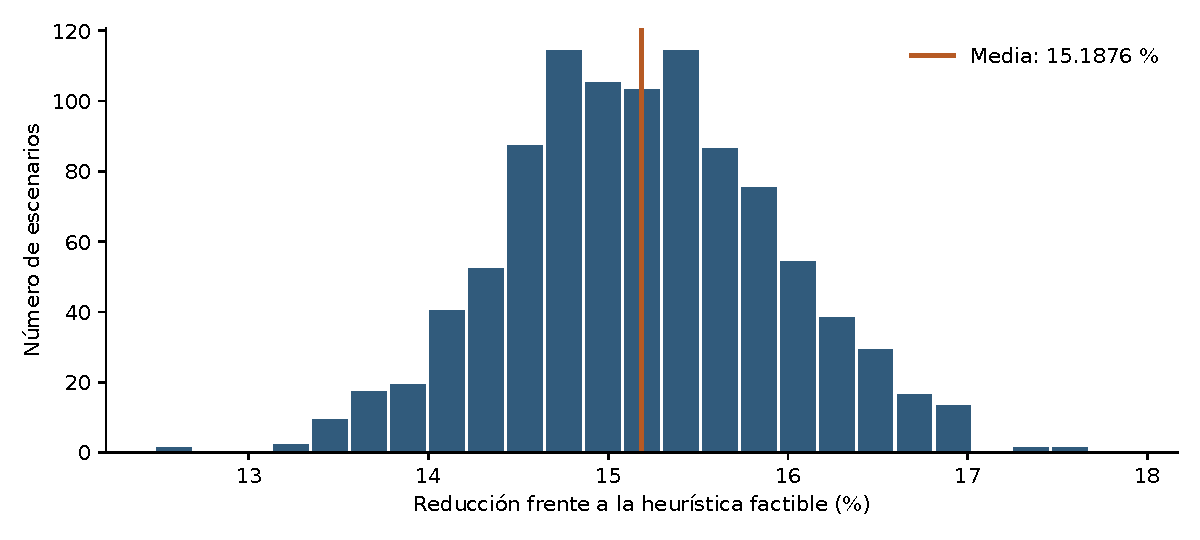
\includegraphics[width=\linewidth]{figuras/monte_carlo_mejora.pdf}
\caption{Distribución de la mejora de los incumbentes en los 1.000 escenarios históricos. La línea señala la media de la muestra.}
\fuente{recálculo a partir de \texttt{monte\_carlo\_escenarios.csv}; no corresponde a una nueva ejecución de los solvers}
\end{figure}

La concentración de la distribución no demuestra que toda demanda futura produzca una mejora semejante. Todos los escenarios provienen de una misma matriz nominal, una capacidad fija y una familia estrecha de perturbaciones. La dispersión observada combina variación del problema y calidad de las soluciones obtenidas dentro del presupuesto histórico.

La figura~\ref{fig:mcgap} permite inspeccionar la relación entre volumen y mejora, y la distribución de brechas. No se ajusta una ley causal entre volumen y rendimiento: los escenarios cambian simultáneamente las demandas de muchas referencias y, con ellas, la combinación de cargas y preparaciones.
\begin{figure}[H]\centering
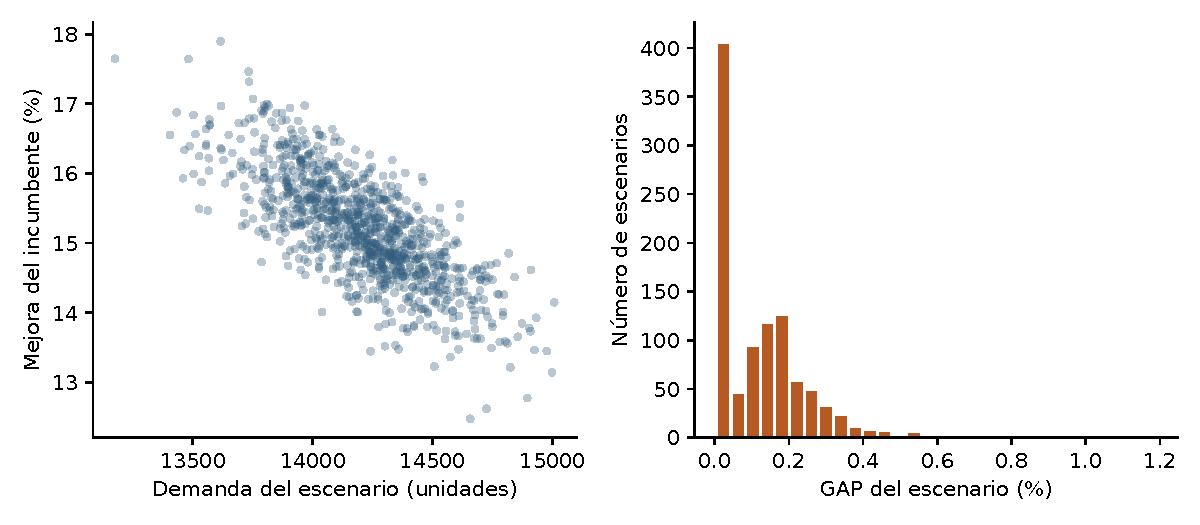
\includegraphics[width=\linewidth]{figuras/monte_carlo_gap.pdf}
\caption{Demanda respecto a mejoras y brechas finales de los escenarios. Cada punto representa una comparación factible.}\label{fig:mcgap}
\end{figure}

\subsection{Incertidumbre de muestreo e incertidumbre de optimización}
Si $LB_s\leq Z_s^*\leq UB_s$, la mejora frente a la heurística queda acotada por
\begin{equation}
100\left(1-\frac{UB_s}{E_s}\right)\leq R_s^*
\leq100\left(1-\frac{LB_s}{E_s}\right).
\end{equation}
La mejora que un plan factible ha logrado se sitúa en el extremo inferior. El extremo superior representa la mayor mejora compatible con la cota inferior del solver. En la muestra, el promedio de esos extremos se sitúa en [15,2\%; 15,3\%]. La incertidumbre residual de optimización con relación a la mejora media de los escenarios se cuantifica con una amplitud de 0,1043 puntos porcentuales.

Se ha anotado un GAP medio del 0,1229\% y uno máximo del 1,1879\%. Ningún escenario presenta un valor numéricamente nulo. Las cotas delimitan la mejora todavía posible, pero no permiten afirmar que el experimento haya certificado mil óptimos. Es una precaución que se une a un balance positivo: en todos los casos de la muestra los incumbentes factibles tienen ya una carga inferior a la heurística.

Un intervalo t de 95\% aproximado se mantiene para la media de las mejoras de los incumbentes:
\begin{equation}
\overline R\ \pm\ t_{0,975;999}\frac{s_R}{\sqrt{1000}}
=[15,1397\%;15,2355\%].
\end{equation}
Bajo el diseño de partida, este intervalo se debe a la variabilidad en la simulación. No tiene por objeto cubrir el error de imputación de los tiempos, las correlaciones que se hayan pasado por alto, las paradas reales o la mejora pendiente entre $UB$ y $LB$. De igual modo, no es un intervalo aplicable a cada escenario por su cuenta. Que coexista con las cotas de mejora no es contradictorio, pues son fuentes de incertidumbre distintas.

\subsection{Reoptimización frente a robustez de un plan fijo}
En cada escenario se puede modificar la asignación una vez que se conoce la demanda. Con el experimento se mide en qué medida la regla de planificación es capaz de adaptarse a las perturbaciones, no la resistencia de un plan nominal sin retoques. Si de lo que se tratara fuera de evaluar un plan fijo habría que ceñirse a las decisiones y cuantificar los excesos de capacidad, faltantes o acciones correctivas que se den en cada caso.

La optimización robusta da forma a unas decisiones amparadas contra conjuntos de incertidumbre, a cambio de un compromiso entre protección y el desempeño nominal \cite{bertsimas}. No se ha puesto en práctica ese procedimiento. La simulación de por sí es un análisis de sensibilidad reiterado y no cabe llamarla modelo robusto de modo automático por el hecho de haber contemplado mil demandas.

Para RPM, el resultado es una ventaja nominal consistente frente a la heurística dentro del diseño de simulación. Para pasar de ahí a una recomendación en condiciones de riesgo operativo harían falta distribuciones o conjuntos de incertidumbre con base en datos, un criterio de servicio y una política de reacción. Esta comparación muestra tales requisitos sin adjudicarles resultados que no se han calculado.

% !TeX root = ../Trabajo_RPM.tex
\subsection{Arquitectura funcional y trazabilidad}
El separador que realiza dicha aplicación es: lectura de entradas, modelado, ejecución del optimizador, verificación y exportación. Su código se puede inspeccionar para dar cuenta de tal separación del flujo, aunque no quiere decir que esto sustituya a la realización de una prueba de disponibilidad en un entorno de producción. Streamlit es responsable de la interfaz; los módulos de cálculo almacenan datos y resultados de una corrida.

La trazabilidad vincula los resultados con una huella de datos y de configuración. De haber un cambio en la demanda, la capacidad o la matriz de tiempos, el plan que se ve ya no se ajustará a la nueva petición. El código identifica esa discrepancia antes de asociar los registros guardados con las nuevas entradas. La sesión de Streamlit guarda la información de unas interacciones a otras \cite{streamlit} y en los archivos exportados queda constancia reproducible. Que un archivo tenga un nombre coincidente no significa por ello que su contenido sea el mismo.

\subsection{Carga de datos y controles previos}
La estructura de carga distingue referencias y recursos. En las primeras se declaran el identificador, la demanda y los tiempos de procesamiento de cada máquina; en los segundos figuran las máquinas, los alistamientos y las capacidades. La plantilla que se puede descargar pone en orden tales campos sin plantear escenarios simulados como si de datos observados se tratara. Para las unidades y las reglas de relleno hay una guía aparte.

La validación comprueba que la demanda sea entera y no negativa, que la identificación sea coherente, que haya correspondencia entre columnas y recursos, así como que los valores de capacidad y preparación sean de los admitidos. Deberán regirse por las normas del formato los tiempos faltantes o combinaciones incompatibles. Hay que tener en cuenta que en el modo de carga donde un cero desactiva una combinación, ese cero no es sinónimo de producción instantánea. Tal convención de la interfaz no viene a alterar los coeficientes positivos de las instancias nominales certificadas.

\subsection{Horizonte automático y certificado}
El modo automático mantiene fija la demanda total y se establecen cotas para el número de días. Un plan que sea viable aporta una cota superior al horizonte; de lo contrario, una condición de carga o una prueba de infactibilidad son necesarias para subir la inferior. Hasta que no haya coincidencia entre ambas el mínimo queda en suspenso. En esa búsqueda puede ser de utilidad presentar un plan descargable cuando su estado denota que el costo o el horizonte mínimo carecen aún de certificación.

La versión revisada retira el selector manual del horizonte. Para el lote nominal mantiene las 45.987 unidades y determina el mínimo de tres días; la tabla de certificación utiliza ese valor junto al caso diario. El modelo optimiza después la carga para el horizonte demostrado. La demanda no aumenta durante la búsqueda de días.

En las repeticiones los horizontes se dejan claros y no se hacen duplicados de filas cuando el de búsqueda coincide con uno ya seleccionado. De ser descartado un horizonte por una cota matemática antes de poner en marcha el solver, se anota como inviabilidad demostrada por cota. A dicha fila no se le asigna un tiempo de optimización de ficción ni se considera una repetición computacional más.

\begin{table}[H]\centering\small
\caption{Estados que deben diferenciarse al consultar la aplicación}
\begin{tabular}{p{43mm}p{56mm}p{46mm}}\toprule
Estado & Interpretación & Uso del archivo\\\midrule
Plan factible de búsqueda & Existe una asignación validada; puede faltar prueba de costo o de mínimo de días & Revisión de carga y alternativa provisional\\
Costo óptimo certificado & Cierre de cotas y plan verificado para el horizonte indicado & Evidencia de asignación óptima nominal\\
Mínimo de días demostrado & Se excluyeron horizontes menores y existe plan en el indicado & Justificación de ventana mínima\\
Inviable demostrado & No existe plan bajo las condiciones examinadas & Revisar demanda, compatibilidad o capacidad\\
Interrumpida o sin conclusión & La ejecución no completó la prueba requerida & Conservar registros sin atribuir certificado\\\bottomrule
\end{tabular}
\end{table}

\subsection{Resultados visibles y archivos de respaldo}
La vista principal muestra la demanda resuelta, los días, el estado y la carga. Los gráficos presentan utilización y holgura por máquina y día; la tabla identifica referencia, máquina, día y cantidad. La preparación por activación figura separada del procesamiento.

El Excel del plan reúne asignaciones, capacidades y estado. El de comparación registra corridas, motor, repetición, semilla, cotas, brechas, duración y auditoría. El comprimido conserva entradas, configuración y registros nativos para revisar planes y reproducir los resultados.

Las credenciales de Gurobi se guardan en la configuración segura, fuera de entradas y archivos exportados. La versión, los parámetros y el log sustentan la identificación del motor.

\subsection{Uso gerencial e implantación gradual}
El supervisor revisa el plan propuesto frente a las restricciones de planta que el modelo no incorpora. Una incompatibilidad exige actualizar los datos y ejecutar otra corrida. Si cambia las cantidades, el certificado original deja de respaldar el plan editado hasta una nueva verificación y optimización.

\end{document}
